
% To do: Check optimilaity claims

\documentclass[10pt, conference, letterpaper]{IEEEtran}



%
% If IEEEtran.cls has not been installed into the LaTeX system files,
% manually specify the path to it like:
% \documentclass[10pt,journal,compsoc]{../sty/IEEEtran}


% Some very useful LaTeX packages include:
% (uncomment the ones you want to load)


% *** MISC UTILITY PACKAGES ***
%
%\usepackage{ifpdf}
% Heiko Oberdiek's ifpdf.sty is very useful if you need conditional
% compilation based on whether the output is pdf or dvi.
% usage:
% \ifpdf
%   % pdf code
% \else
%   % dvi code
% \fi
% The latest version of ifpdf.sty can be obtained from:
% http://www.ctan.org/tex-archive/macros/latex/contrib/oberdiek/
% Also, note that IEEEtran.cls V1.7 and later provides a builtin
% \ifCLASSINFOpdf conditional that works the same way.
% When switching from latex to pdflatex and vice-versa, the compiler may
% have to be run twice to clear warning/error messages.

\usepackage{upgreek}
% *** CITATION PACKAGES ***
%
\ifCLASSOPTIONcompsoc
  % IEEE Computer Society needs nocompress option
  % requires cite.sty v4.0 or later (November 2003)
  \usepackage[nocompress]{cite}
\else
  % normal IEEE
  \usepackage{cite}
\fi


% cite.sty was written by Donald Arseneau
% V1.6 and later of IEEEtran pre-defines the format of the cite.sty package
% \cite{} output to follow that of IEEE. Loading the cite package will
% result in citation numbers being automatically sorted and properly
% "compressed/ranged". e.g., [1], [9], [2], [7], [5], [6] without using
% cite.sty will become [1], [2], [5]--[7], [9] using cite.sty. cite.sty's
% \cite will automatically add leading space, if needed. Use cite.sty's
% noadjust option (cite.sty V3.8 and later) if you want to turn this off
% such as if a citation ever needs to be enclosed in parenthesis.
% cite.sty is already installed on most LaTeX systems. Be sure and use
% version 5.0 (2009-03-20) and later if using hyperref.sty.
% The latest version can be obtained at:
% http://www.ctan.org/tex-archive/macros/latex/contrib/cite/
% The documentation is contained in the cite.sty file itself.
%
% Note that some packages require special options to format as the Computer
% Society requires. In particular, Computer Society  papers do not use
% compressed citation ranges as is done in typical IEEE papers
% (e.g., [1]-[4]). Instead, they list every citation separately in order
% (e.g., [1], [2], [3], [4]). To get the latter we need to load the cite
% package with the nocompress option which is supported by cite.sty v4.0
% and later. Note also the use of a CLASSOPTION conditional provided by
% IEEEtran.cls V1.7 and later.
% *** GRAPHICS RELATED PACKAGES ***
%
\ifCLASSINFOpdf
   \usepackage[pdftex]{graphicx}
   \usepackage{subfigure}
  % declare the path(s) where your graphic files are
  % \graphicspath{{../pdf/}{../jpeg/}}
  % and their extensions so you won't have to specify these with
  % every instance of \includegraphics
  % \DeclareGraphicsExtensions{.pdf,.jpeg,.png}
\else
  % or other class option (dvipsone, dvipdf, if not using dvips). graphicx
  % will default to the driver specified in the system graphics.cfg if no
  % driver is specified.
   \usepackage[dvips]{graphicx}
   \usepackage{subfigure}
  % declare the path(s) where your graphic files are
  % \graphicspath{{../eps/}}
  % and their extensions so you won't have to specify these with
  % every instance of \includegraphics
  % \DeclareGraphicsExtensions{.eps}
\fi


% graphicx was written by David Carlisle and Sebastian Rahtz. It is
% required if you want graphics, photos, etc. graphicx.sty is already
% installed on most LaTeX systems. The latest version and documentation
% can be obtained at: 
% http://www.ctan.org/tex-archive/macros/latex/required/graphics/
% Another good source of documentation is "Using Imported Graphics in
% LaTeX2e" by Keith Reckdahl which can be found at:
% http://www.ctan.org/tex-archive/info/epslatex/
%
% latex, and pdflatex in dvi mode, support graphics in encapsulated
% postscript (.eps) format. pdflatex in pdf mode supports graphics
% in .pdf, .jpeg, .png and .mps (metapost) formats. Users should ensure
% that all non-photo figures use a vector format (.eps, .pdf, .mps) and
% not a bitmapped formats (.jpeg, .png). IEEE frowns on bitmapped formats
% which can result in "jaggedy"/blurry rendering of lines and letters as
% well as large increases in file sizes.
%
% You can find documentation about the pdfTeX application at:
% http://www.tug.org/applications/pdftex
% *** MATH PACKAGES ***
%
\usepackage[cmex10]{amsmath}
\usepackage{amssymb}
 \usepackage{graphicx}
 \usepackage{epstopdf}
  \usepackage{tabulary}
  \usepackage{array,booktabs,longtable,tabularx}
% A popular package from the American Mathematical Society that provides
% many useful and powerful commands for dealing with mathematics. If using
% it, be sure to load this package with the cmex10 option to ensure that
% only type 1 fonts will utilized at all point sizes. Without this option,
% it is possible that some math symbols, particularly those within
% footnotes, will be rendered in bitmap form which will result in a
% document that cannot be IEEE Xplore compliant!
%
% Also, note that the amsmath package sets \interdisplaylinepenalty to 10000
% thus preventing page breaks from occurring within multiline equations. Use:
%\interdisplaylinepenalty=2500
% after loading amsmath to restore such page breaks as IEEEtran.cls normally
% does. amsmath.sty is already installed on most LaTeX systems. The latest
% version and documentation can be obtained at:
% http://www.ctan.org/tex-archive/macros/latex/required/amslatex/math/
% *** SPECIALIZED LIST PACKAGES ***
%
\usepackage[justification=centering]{caption}
\usepackage{url}
\usepackage{amsmath}
\usepackage{amsfonts}
\newtheorem{definition}{\noindent{\bf Definition}}
\newtheorem{lemma}{\noindent{\bf Lemma}}
\newtheorem{theorem}{\noindent{\bf Theorem}}
\newtheorem{proposition}{\noindent{\bf proposition}}



\usepackage{algorithm}
\usepackage{algorithmic}
% algorithmic.sty was written 

\usepackage{eqparbox}

\renewcommand{\algorithmiccomment}[1]{\hfill\eqparbox{COMMENT}{\%~#1}}




\begin{document}

\title{ Yosemite: Efficient Scheduling of Weighted Coflows in Data Centers}
%\author{\IEEEauthorblockN{Han Zhang\IEEEauthorrefmark{1}\IEEEauthorrefmark{3},  Xingang Shi\IEEEauthorrefmark{2}\IEEEauthorrefmark{3}, Xia Yin\IEEEauthorrefmark{1}\IEEEauthorrefmark{3}, Zhiliang Wang\IEEEauthorrefmark{2}\IEEEauthorrefmark{3},YingYa Guo\IEEEauthorrefmark{1}\IEEEauthorrefmark{3}}
%\IEEEauthorblockA{\IEEEauthorrefmark{1}Department of Computer Science and Technology, Tsinghua University\\
%\IEEEauthorrefmark{2}Institute for Network Sciences and Cyberspace, Tsinghua University\\
%\IEEEauthorrefmark{3}Tsinghua National Laboratory for Information Science and Technology (TNLIST)\\
%Beijing, P.R. China\\
%Email:\{zhanghan, wzl, yxia,guoyingya\}@csnet1.cs.tsinghua.edu.cn, \{shixg\}@cernet.edu.cn
%}
%}
\author{Paper ID: \#1570386872}
% make the title area
\maketitle



\begin{abstract}
Traditional network resource allocation or scheduling mechanisms are mainly flow or packet based.
Recently, coflow has been proposed as a new abstraction to capture the communication patterns in a rich set of data parallel applications in data centers. Coflows effectively model the application-level semantics of network resource usage, so high-level optimization goals, such as reducing the transfer latency of applications, can be better achieved by taking coflows as the basic elements in network resource allocation or scheduling.
Although efficient coflow scheduling methods have been studied in this aspect, in this paper, we propose to schedule {\em weighted coflows} as a further step in this direction, where weights are used to express the emergences or priorities of different coflows or their corresponding applications. We introduce the Weighted Coflow Completion Time (WCCT) minimization problem, and design an information-agnostic online algorithm to dynamically schedule cflows according to their weights and the instantaneous network condition. We implement the algorithm in a scheduling system named Yosemite, and evaluate its performance by trace-driven simulations as well as real deplopyment in a cloud testbed. Our evaluation results show that, compared to the latest information-agnostic coflow scheduling algorithms, Yosemite can reduce more than 40\% of the WCCT, and more than 30\% of the completion time for coflows with above-the-average level of emergence. It even outperforms the most efficient clairvoyant coflow scheduling method by reducing around 30\% WCCT, and 20\%$\sim$30\% of the completion time for coflows with above-the-average emergence, respectively. %Nowadays, applications (hadoop, ceph, etc.) in data center need network to provide them with low latency and high throughput. 
%However, as resources of data center network are limited, efficient network schedule methods are needed. Recently, the proposed
%application level abstraction coflow tries to regard flows of data-parallel applications as a whole, so that transfer latency of applications will be reduced. 
%For reducing application transfer latency, application level optimization methods perform better than flow level ones.
%This is because often a application's communication stage cannot finish until all its flows have completed. 
%Although coflow level scheduling methods such as Varys and Aalo perform well on reducing application transfer latency,
%they ignore different applications always have different level of emergence and 
%scheduling just depends on network condition and characters (width, length) of coflows is not enough.
%In reality, the emergence of applications should also be taken into consideration.
%In this paper, we incorporate weight to present the emergence of applications and try to minimize average coflow weight completion time.
%To achieve this, we design Yosemite-a system that aims to minimize average weight coflow completion time.
%We test Yosemite's performance in trace-driven simulation as well as our cloud platform and then compare its performance with state-of-art methods.  
%Trace-driven simulation shows that Yosemite performs about 20\%$\sim$50\%better than Varys and 30\%$\sim$60\% better than Aalo. 
%Testbed evaluation shows Yosemite performs  30\% and 35\% better than Varys and Aalo respectively on average.
\end{abstract}

\section{Introduction}\label{introduction}

Nowadays, low latency\cite{Latency}\cite{munir2014friends} and high throughput\cite{CloudMirror} are required by data center applications, for example, 
those with map-reduce style data-intensive computing \cite{dean2008mapreduce}, and those using distributed file storage\cite{lin2010secure}\cite{dimakis2006decentralized}, etc.
To meet these requirements, the data center networking infrastructure has been specially tailored, with a tremendous amount of efforts to improve the network topology and routing schemes, as well as transport schemes. 

Among these efforts, flow level scheduling methods try to schedule arriving packets according to the characteristics of the corresponding flows. For example, PDQ\cite{PDQ} and pFabric\cite{pFabric} approximate the {\em shortest job first} (SJF) policy to let shorter flows preempt the bandwidth of longer ones. 
As a result, the average Flow Completion Time (FCT) tends to be reduced, so does applications' transport latency. 
However, since the communication of an application cannot finish until all its flows have completed their transmission, the overall transport performance of an application may not be effectively improved, or may even be impaired, by scheduling individual flows without considering their inter-relationship.
% still have several deficiencies\cite{chowdhury2011managing}. 
%On the one hand, flow level scheduling has to be carried out quite frequently, such that centralized scheduler may face huge pressure on its own computation and communication, while decentralized scheduler may face worse scheduling performance.
%On the other hand, some tardy flows 

Recently, coflow has been proposed as a new abstraction to capture the communication patterns in a rich set of data parallel applications.
According to \cite{chowdhury2012coflow}, a coflow is {\em a collection of flows between two groups of machines with associated semantics and a collective objective.} The collection of flows share a common performance goal, e.g., minimizing the completion time of the latest flow in the collection, or ensuring that flows in the collection meet a common deadline. 
Coflows effectively model the application-level semantics of network resource usage, so high-level optimization goals, such as reducing the transfer latency of applications, can be better achieved by taking coflows as the basic elements in network resource allocation or scheduling.
Efficient coflow scheduling methods targeting minimizing Coflow Completion Time (CCT) have been studied. 
Varys \cite{chowdhury2014efficient} proposes the {\em Smallest-Effective-Bottleneck-First} (SEBF) heuristic to determine the scheduling order of coflows and uses {\em Minimum-Allocation-for-Desired-Duration} (MADD) to compute the bandwidth to be allocated. However, Varys is a clairvoyant method in the sense that it depends on flow information, such as flow size or flow arrival time, to determine how to scheduling coflows. This may limit its application to scenarios where such information cannot be provided a priori. To solve this problem, non-clairvoyant methods that are flow information agnostic, such as Aalo \cite{chowdhury2015efficient}, Barrat \cite{dogar2014decentralized}, sunflows \cite{huang2016sunflow} and CODA \cite{zhang2016coda}, have also been studied.

%Indeed, both Non-clairvoyant and clairvoyant only consider network condition, but ignore the emergence of coflows.
%According to our measurement and analysis, we find in data center, applications have different level of emergence, and only depending on network condition is not enough.
%the emergence of coflow should also be taken into consideration.

In this paper, we propose to schedule {\em weighted coflows} as a further step in this direction, where weights are assigned to coflows to express the emergences or priorities of different coflows or their corresponding applications. 
%In this paper, we assign weight to coflow to present its importance and propose {\em weighted coflows} as a further step in this direction, where important coflows have higher weight and unimportant ones have lower value. 
%This is natural since there exist both delay sensitive and insensitive applications, and some 
%applications may gain (or lose) more revenue than others in the same amount of time.
For example, supporting the internal communication requirement of a search engine with intense internal computation should be more emergent than supporting the file backup on a distributed storage system. When scheduling coflows from these two applications, we would like to take this difference into consideration. To accomplish this, we assign different weights to them, i.e., coflows of search engine have a higher weight, while coflows of file backup have a lower weight, and try to minimize the Weighted Coflow Completion Time (WCCT), which is the weighted summation of the completion time of all coflows.
%When deciding the scheduling sequence, we consider both network condition and coflow weight. 
%On this condition, weighted coflow completion time (WCCT) is set as the optimization target. 

We formulate an Idealized Weighted Coflow Completion Time Minimization (IWCCTM) problem, and prove that one of its special cases is equivalent to minimizing the weighted job completion time in the concurrent open shop problem \cite{mastrolilli2010minimizing}, which is known to be NP-hard. Following the idea presented in \cite{mastrolilli2010minimizing}, we derive for IWCCTM a non-preemptive scheduling algorithm that is 2-approximate optimal. To make it more practical, we then convert it to an information-agnostic algorithm, which introduces only minor performance loss, but can schedule coflows online without knowing their size or arrival time a priori. We further design and implement a scheduling system named Yosemite using the scala language. Yosemite relies on the Akka \cite{Akka} and kryo \cite{kryo} libraries, and can readily be deployed in a productional cloud environment like openstack. We have extensively tested the performance of Yosemite by both trace-driven simulations and testbed evaluations, and compare it against state-of-the-art coflow scheduling algorithms with best known performance, such as Varys \cite{chowdhury2014efficient} , Aalo \cite{chowdhury2015efficient} and Barrat \cite{dogar2014decentralized}. The corresponding results show that Yosemite performs quite effectively in reducing the Weighted Coflow Completion Time. 

%where Yosemite performs quite well in reducing the weighted coflow completion time. Our trace-driven simulations show that, Yosemite's online scheduling algorithm performs about 20\%$\sim$50\% and 30\%$\sim$60\% better than that of Varys and Aalo, respectively. And in our testbed evaluations, Yosemite achieves 30\%  average improvement against Varys.

Our contributions in this paper are summarized as follows:

\begin{itemize}[\IEEEsetlabelwidth{Z}]
\item We are the first to propose the scheduling of {\em weighted coflows} as an essential network resource management scheme in data centers hosting multiple kinds of applications. We collect real application traffic from a medium-sized data center and make an in-depth analysis to reveal the importance of weighted coflow scheduling.

%measure our data centers' traffic and find it insufficient to schedule coflows just relying on network condition, importance of coflow should also be taken into consideration.

\item We formulate an Idealized Weighted Coflow Completion Time Minimization (IWCCTM) problem, study its hardness, and derive a non-preemptive scheduling algorithm that is 2-approximate optimal. 
%prove its equivalence to the job weighted completion time problem in the concurrent open shop setting.
\item We further design a practical information-agnostic algorithm and build the Yosemite system to minimize WCCT in real environment. Yosemite can readily be deployed in a cloud environment like openstack. 

\item Our evaluation results show that, compared to the latest information-agnostic coflow scheduling algorithms, Yosemite can reduce more than 40\% of the WCCT, and more than 30\% of the completion time for coflows with above-the-average level of emergence. It even outperforms the most efficient clairvoyant coflow scheduling method by reducing around 30\% WCCT, and 20\%$\sim$30\% of the completion time for coflows with above-the-average emergence, respectively. 

\end{itemize}

The rest of the paper is organized as follows. Section \ref{background} introduces the related work and our motivation. Section \ref{system model} formulates the WCCT minimization problem and discusses its hardness. Section \ref{algorithm} presents our information-agnostic coflow scheduling algorithm and the practical Yosemite system in detail.  Section \ref{evaluation} evaluates Yosemite against several coflow scheduling methods, and Section \ref{conclusion} concludes.


\section{Background and Motivation}\label{background}
Data center is now becoming an important facility for hosting a large number of services and applications. To meet their demands of high throughput and low latency, a tremendous amount of  research effort has been devoted to network resource allocation. For example, DCTCP\cite{DCTCP}, D$^2$TCP\cite{D2TCP}, L$^2$DCT \cite{L2DCT} , LPD \cite{zhang2015more} ,D3 \cite{D3} and PDQ \cite{PDQ} are flow level rate control or scheduling schemes aiming to minimize the Flow Completion Time (FCT) or to meet strict flow deadlines. The concept of coflow has recently been proposed \cite{chowdhury2012coflow} to meet the application performance requirement at a higher level, where a coflow is a collection of flows between two groups of machines with associated semantics and a collective objective. Algorithms are also devised to schedule coflows to minimize the Coflow Completion Time (CCT), and are of the most relevance to our problem. In particular, 
%Barrat \cite{dogar2014decentralized} schedules tasks in a FIFO fashion, 
Varys computes network bottleneck based on flow size and applies its {\em Effective-Bottleneck-First} heuristic, while D-CLAS\cite{chowdhury2015efficient}, Aalo\cite{luo2016towards}, sunflows\cite{huang2016sunflow} and CODA \cite{zhang2016coda} try to "guess" various characterics of coflows in different ways to help scheduling. The former is often called a clairvoyant method in the sense that it explicitly depends on flow information like size and arrival time, while the latter four are flow information agnostic.

%Indeed, both the implicit and explicit methods are all flow-level optimization methods.
%Having recognized limitation of flow-level methods, application level schedule methods occur. 
%Barrat \cite{dogar2014decentralized}  schedules tasks in FIFO order but avoids head-of-line blocking by dynamically changing the level of multiplexing in the network. 
%Using Barrat, each task has a globally unique priority-all flows within the task use this priority, irrespective of when these flows start or which part of the network they traverse. 
%Barrat is simple, but for some large coflow, it can down many smaller ones. 
%Varys \cite{chowdhury2014efficient} regards applications' parallel flows as coflow and it uses SEBF to schedule coflows and MADD to perform rate control, 
%as a result, other coexisting coflows can make progress and the average CCT decreases.
%Varys needs to know coflow length as well as width beforehand.
%Varys is a Clairvoyant schedule method, which means some coflow information such as coflow length and coflow width should be known beforehand.
%Unfortunately, in many cases, coflow characteristics are unknown a priori and this will limit the its utilization.
%Aalo\cite{luo2016towards}, sunflows\cite{ huang2016sunflow},
%D-CLAS\cite{chowdhury2015efficient} and CODA \cite{zhang2016coda} make an advance, they do not need to know coflow information beforehand. 
%They use  information accumulation or machine learning to "guess" the characters of coflow. 
%Non-Clairvoyant methods can be used more widely, however, they tend to have relatively worse performance than Varys.
Although these coflow level scheduling methods indeed effectively improve the communication or data transfer performance, they treat different coflows or applications as equally important. As a result, the difference of performance improvement between different coflows or applications depends on the specific scheduling heuristics. For example, one scheduling scheme may favor short flows, while another may favor coflows with larger width, i.e., consisting of a large number of flows, sometimes even unpredictable or inconsistent. In this sense, we argue that coflows (or applicaitons) often have priorities or emergency levels, and should be explicitly taken into consideration when they are scheduled. For example, supporting the internal communication requirement of a search engine with intense internal computation should be more emergent
than supporting the file backup on a distributed storage system. Although in this example the more emergent coflows mainly consist of short flows and tend to have a large width, this is not always the case, and in general emergency is orthogonal to other physical characteristics. Thus, the scheduling methods introduced above lack the capability to improve the performance of coflows with the strongest demand.


\begin{figure*}[!t]
\centering
\subfigure[Average CCT] {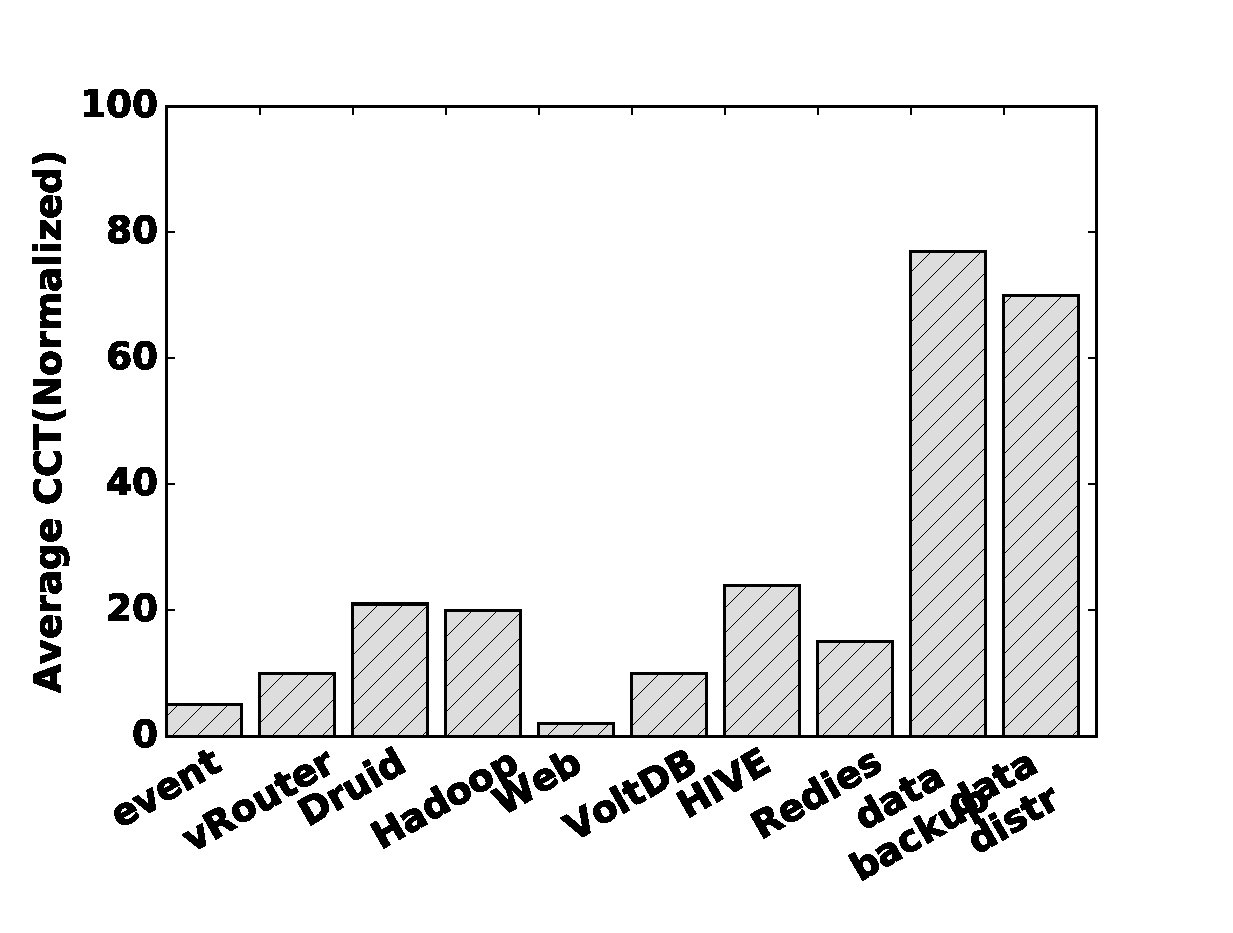
\includegraphics[width=1.65 in]{./figs/motivation/motivation1.eps}}
\hspace{0.1in}
\subfigure[Average CCT with Varys ] {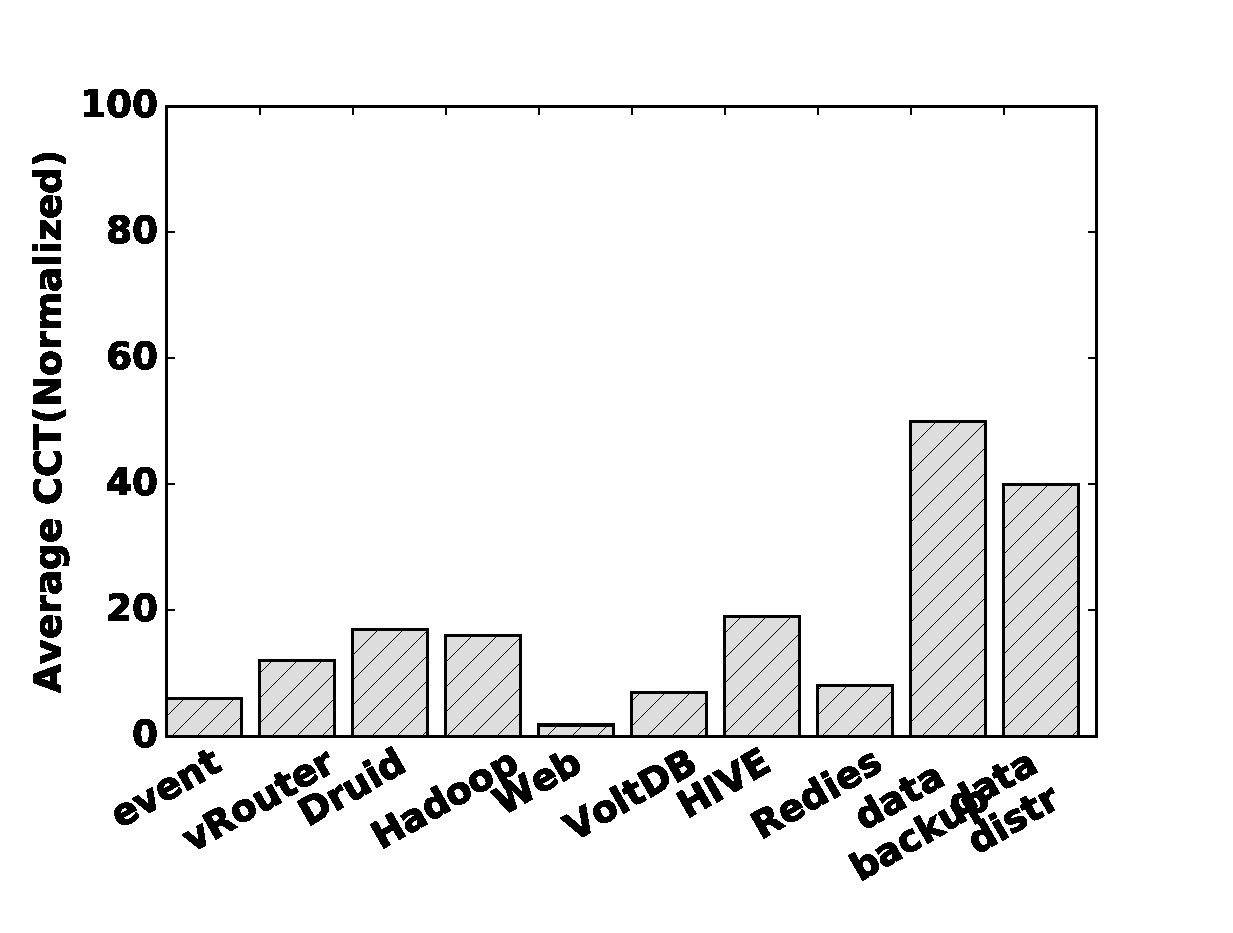
\includegraphics[width=1.65 in]{./figs/motivation/motivation3.eps}}
\hspace{0.1in}
\subfigure[Hadoop CCT ] {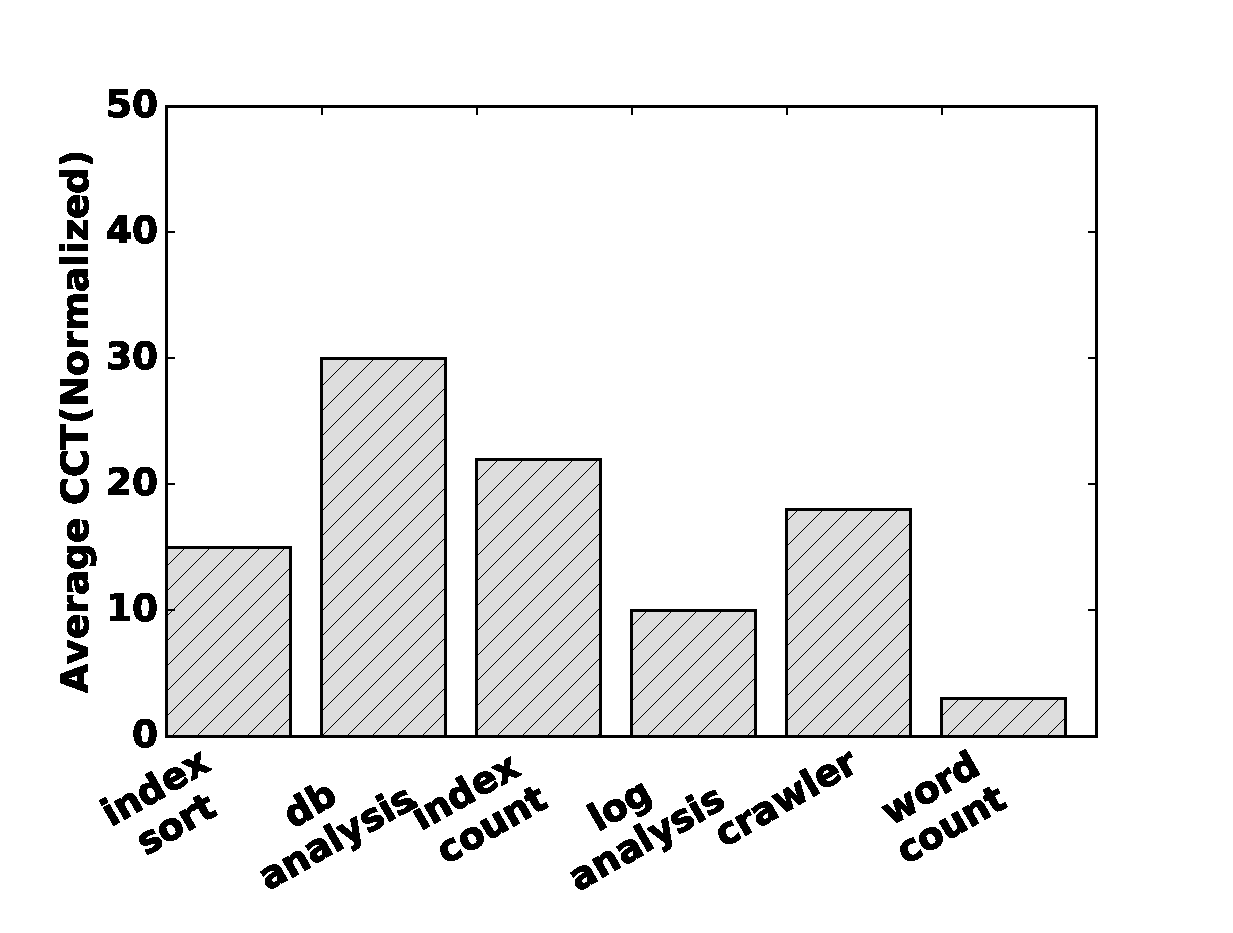
\includegraphics[width=1.65 in]{./figs/motivation/motivation2.eps}}
\vspace{-0.1 in}
\subfigure[Hadoop CCT with Varys ] {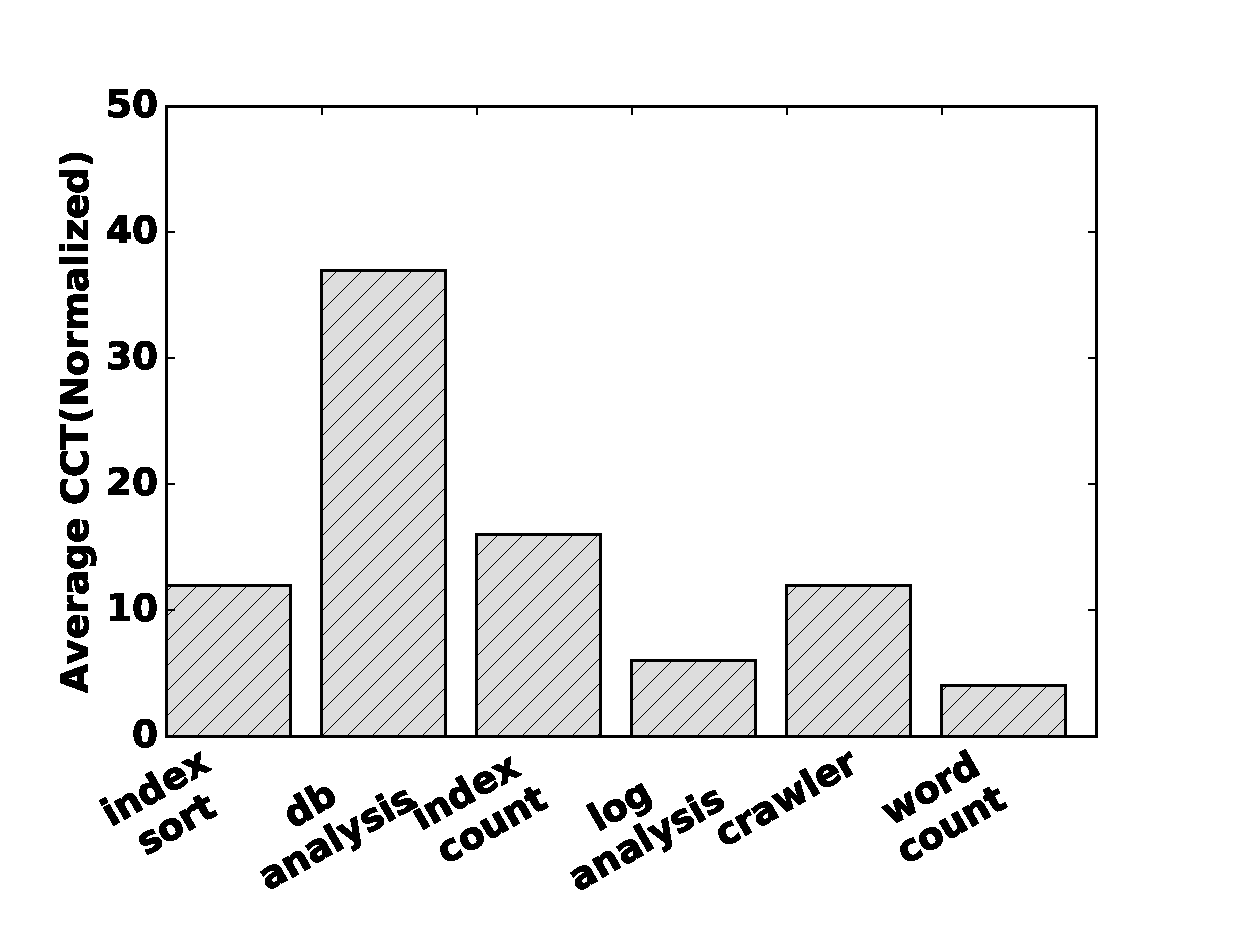
\includegraphics[width=1.65 in]{./figs/motivation/motivation4.eps}}
\hspace{0.1in}
\caption{Normalized Coflow Completion Time, grouped by the level of emergence}
\label{motivation_fig}
\vspace{-0.1 in}
\end{figure*}


 \begin{table}[!htb]
\centering
\footnotesize
 \caption{Applications and their levels of emergence} \label{tab:measure}
\begin{tabulary}{\textwidth}{rccccr}
\toprule
App Name  & \multicolumn{1}{c}{Type} &  width&  length (MB)&Emergence Level\\
\midrule
 \multicolumn{1}{r}{Event} &     communication    &20&5     &  significant \\
 \multicolumn{1}{r}{vRouter} &  communication     &8&3 &  significant\\
\multicolumn{1}{r}{Druid} &     interactive   &6&18   &  important \\
\multicolumn{1}{r}{Hadoop} &  computation  &5&42     &  normal \\
 \multicolumn{1}{r}{Web} &     interactive   &3&5     &  normal\\
\multicolumn{1}{r}{VoltDB} &     background  &4&21    &  normal\\
 \multicolumn{1}{r}{Hive} &     background   &7&32     &  unimportant \\
   \multicolumn{1}{r}{Redies} &    background   &2&30    &  unimportant \\
    \multicolumn{1}{r}{data-backup} &    background   &3&124     &  lax \\
     \multicolumn{1}{r}{data-dist} & background      &5&93  &lax \\
\bottomrule
 \end{tabulary}
 \end{table}


%emphasize on flow level scheduling. 
%%They propose to mark packets on a switch when instantaneous queue length exceeds a certain threshold. 
%%The endpoints then estimate the extent of congestion by the marked packets, and throttle flow rates in proportion to that extent. 
%With the help of ECN marking mechanism, they reduce the queue length on switches, thus cutting transfer latency.
%TCP-based methods are simple, 
%however, they are implicit rate control method \cite{pFabric} and can never precisely estimate the right flow rates to use so as to schedule flows to minimize FCT 
%while ensuring that the network is fully utilized.
%D3 \cite{D3} and PDQ \cite{PDQ} are explicit methods which can schedule flows based on some notion of urgency. 
% A centralized controller which collects the network condition and computes flow bandwidth is needed. 
% Although these methods can assign rates according to flow deadlines or flows' estimated completion time, they can not satisfy the demands of applications well.
% This is because distributed applications always have many parallel flows and often an application's communication stage cannot finish until all its flows have completed.
% If we only focus on single flow scheduling, some tardy flows may finish late and it doesn't make any sense to allocate much bandwidth to the application.
% As a result, scheduling applications' flows as a whole is meaningful.
 
 \begin{table}[!htb]
\centering
\footnotesize
 \caption{Coflows in Hardoop and their levels of emergence} \label{tab:measure2}
\begin{tabulary}{\textwidth}{rcccr}
\toprule
Coflow Type  &  width&length (MB)&Emergence Level\\
\midrule
 \multicolumn{1}{r}{index-sort}       &10&3  &significant \\
 \multicolumn{1}{r}{db-analysis}   &3&12     &  important \\
  \multicolumn{1}{r}{index-count}   &6&20 &  normal\\
\multicolumn{1}{r}{log-analysis}    &6&31   &  unimportant \\
\multicolumn{1}{r}{crawler}   &4&12     &  unimportant \\
    \multicolumn{1}{r}{word-count}    &3&11     &  unimportant\\
   \bottomrule
 \end{tabulary}
 \end{table}
 
To make this argument more convincing, we now use real network traffic from a medium-sized data center, where more than 100 applications run on about 3000 servers simultaneously. After talking with the network operators and software development engineers about the emergence of different applications, we make an in-depth analysis of the traffic collected from 720 servers depolyed in 60 racks. The traffic lasts about one month, and the basic statistics of the top ten network-demanding applications are summarized in Table \ref{tab:measure}. There are typically five emergence levels, i.e., significant, important, normal, unimportant and lax. For example, the event application and the vRoute application are responsible for communication of critical components, and are of the highest level of emergence, while data-backup and data-dist are  applications running in the background and are of the lowest level of emergence. We can see applications consisting of a larger number of flows or smaller flows are not necessarily more emergence. For example, the average number of flows in Hive (i.e., 7) is larger than that of Web (i.e., 3), but Hive is less emergent than Web. Another example is that, the average flow size of Web (i.e. 5) is smaller than that of Druid (i.e., 18), but Web is of less emergence than Druid. This supports our former statement that in general, emergency is orthogonal to other physical characteristics of coflows. Table.\ref{tab:measure2} further shows the details of different coflows in the hadoop application, from which we can make similar conclusions.

To illustrate the ineffectiveness of existing coflow scheduling methods, we plot the average Coflow Completion Time (CCT) of different coflows, grouped by their levels of emergence, in Fig.\ref{motivation_fig}. Fig.\ref{motivation_fig}(a) shows the direct measurement result of all applications, while Fig.\ref{motivation_fig}(b) shows the simulation result when Varys is used to schedule them. Comparing the two plots, we can see that Varys clearly reduces the completion time of less emergent coflows, such as Redies, data-backup and data-dist, at the expenses of the same of even longer completion time of more emergent coflows, such as Event and vRouter. A similar effect can be observed in Fig.\ref{motivation_fig}(c) and Fig.\ref{motivation_fig}(d), where the measured CCTs of Hadoop coflows are compared to the scheduling results of Varys. This motivates us to optimize the Weighted Coflow Completion Time (WCCT), where weight denotes the emergence of coflows, and the more emergent the coflow, the higher the weight. Coflow scheduling algorithms should take coflow weight into consideration, and optimizing CCT becomes just a special case of optimizing WCCT.

%However, methods such as  \cite{qiu2015minimizing} will solve complex equations which make them too complex to use in practice.
%Due to these deficiencies, in this paper, we follow this direction and  proposal 
%There are many methods to present the semantics of the application. 
%Some flow-level algorithms such as D2TCP\cite{D2TCP} and LPD\cite{zhang2015more} use deadline to present the emergency of applications. 
%Flow missing deadline will be threw way. Deadline can guarantee the application to have low bound of bandwidth and it can describe the semantics of application to some extent. 
%However, in data center network, applications do not need a minimum bandwidth or have a strict finish time constraints. 
%They just have higher level of emergency and hope to finish as quickly as possible, so another kind of method to present the emergency of application according to the semantics is needed. \cite{qiu2015minimizing} and \cite{qiu2016experimental} incorporate weight into consideration. 
%They set larger weight to the more emergency jobs. Instead of minimizing coflow completion time, t
%hey try to minimize weight coflow completion time. Comparing with optimizing weight completion time, optimizing weight completion time considers application semantics. 
%They make progress on application bandwidth allocation. However both \cite{qiu2015minimizing} and \cite{qiu2016experimental}
%have high complexity, which make them hard to deploy in practice. In reality, we need the method to compute quickly to react the burst of flows in data center network.  

      
      
      
      


\section{Model and problem formulation}\label{system model}
In this section, we first introduce the non-blocking fabric model to reasonably simplify the coflow scheduling problem in data center networks.Then we formulate an Idealized Weighted Coflow Completion Time Minimization (IWCCTM) problem and discuss its hardness.

\subsection{Non-blocking Fabric Model for Data Center Networks}

%\begin{figure}[b]
%\begin{center}
%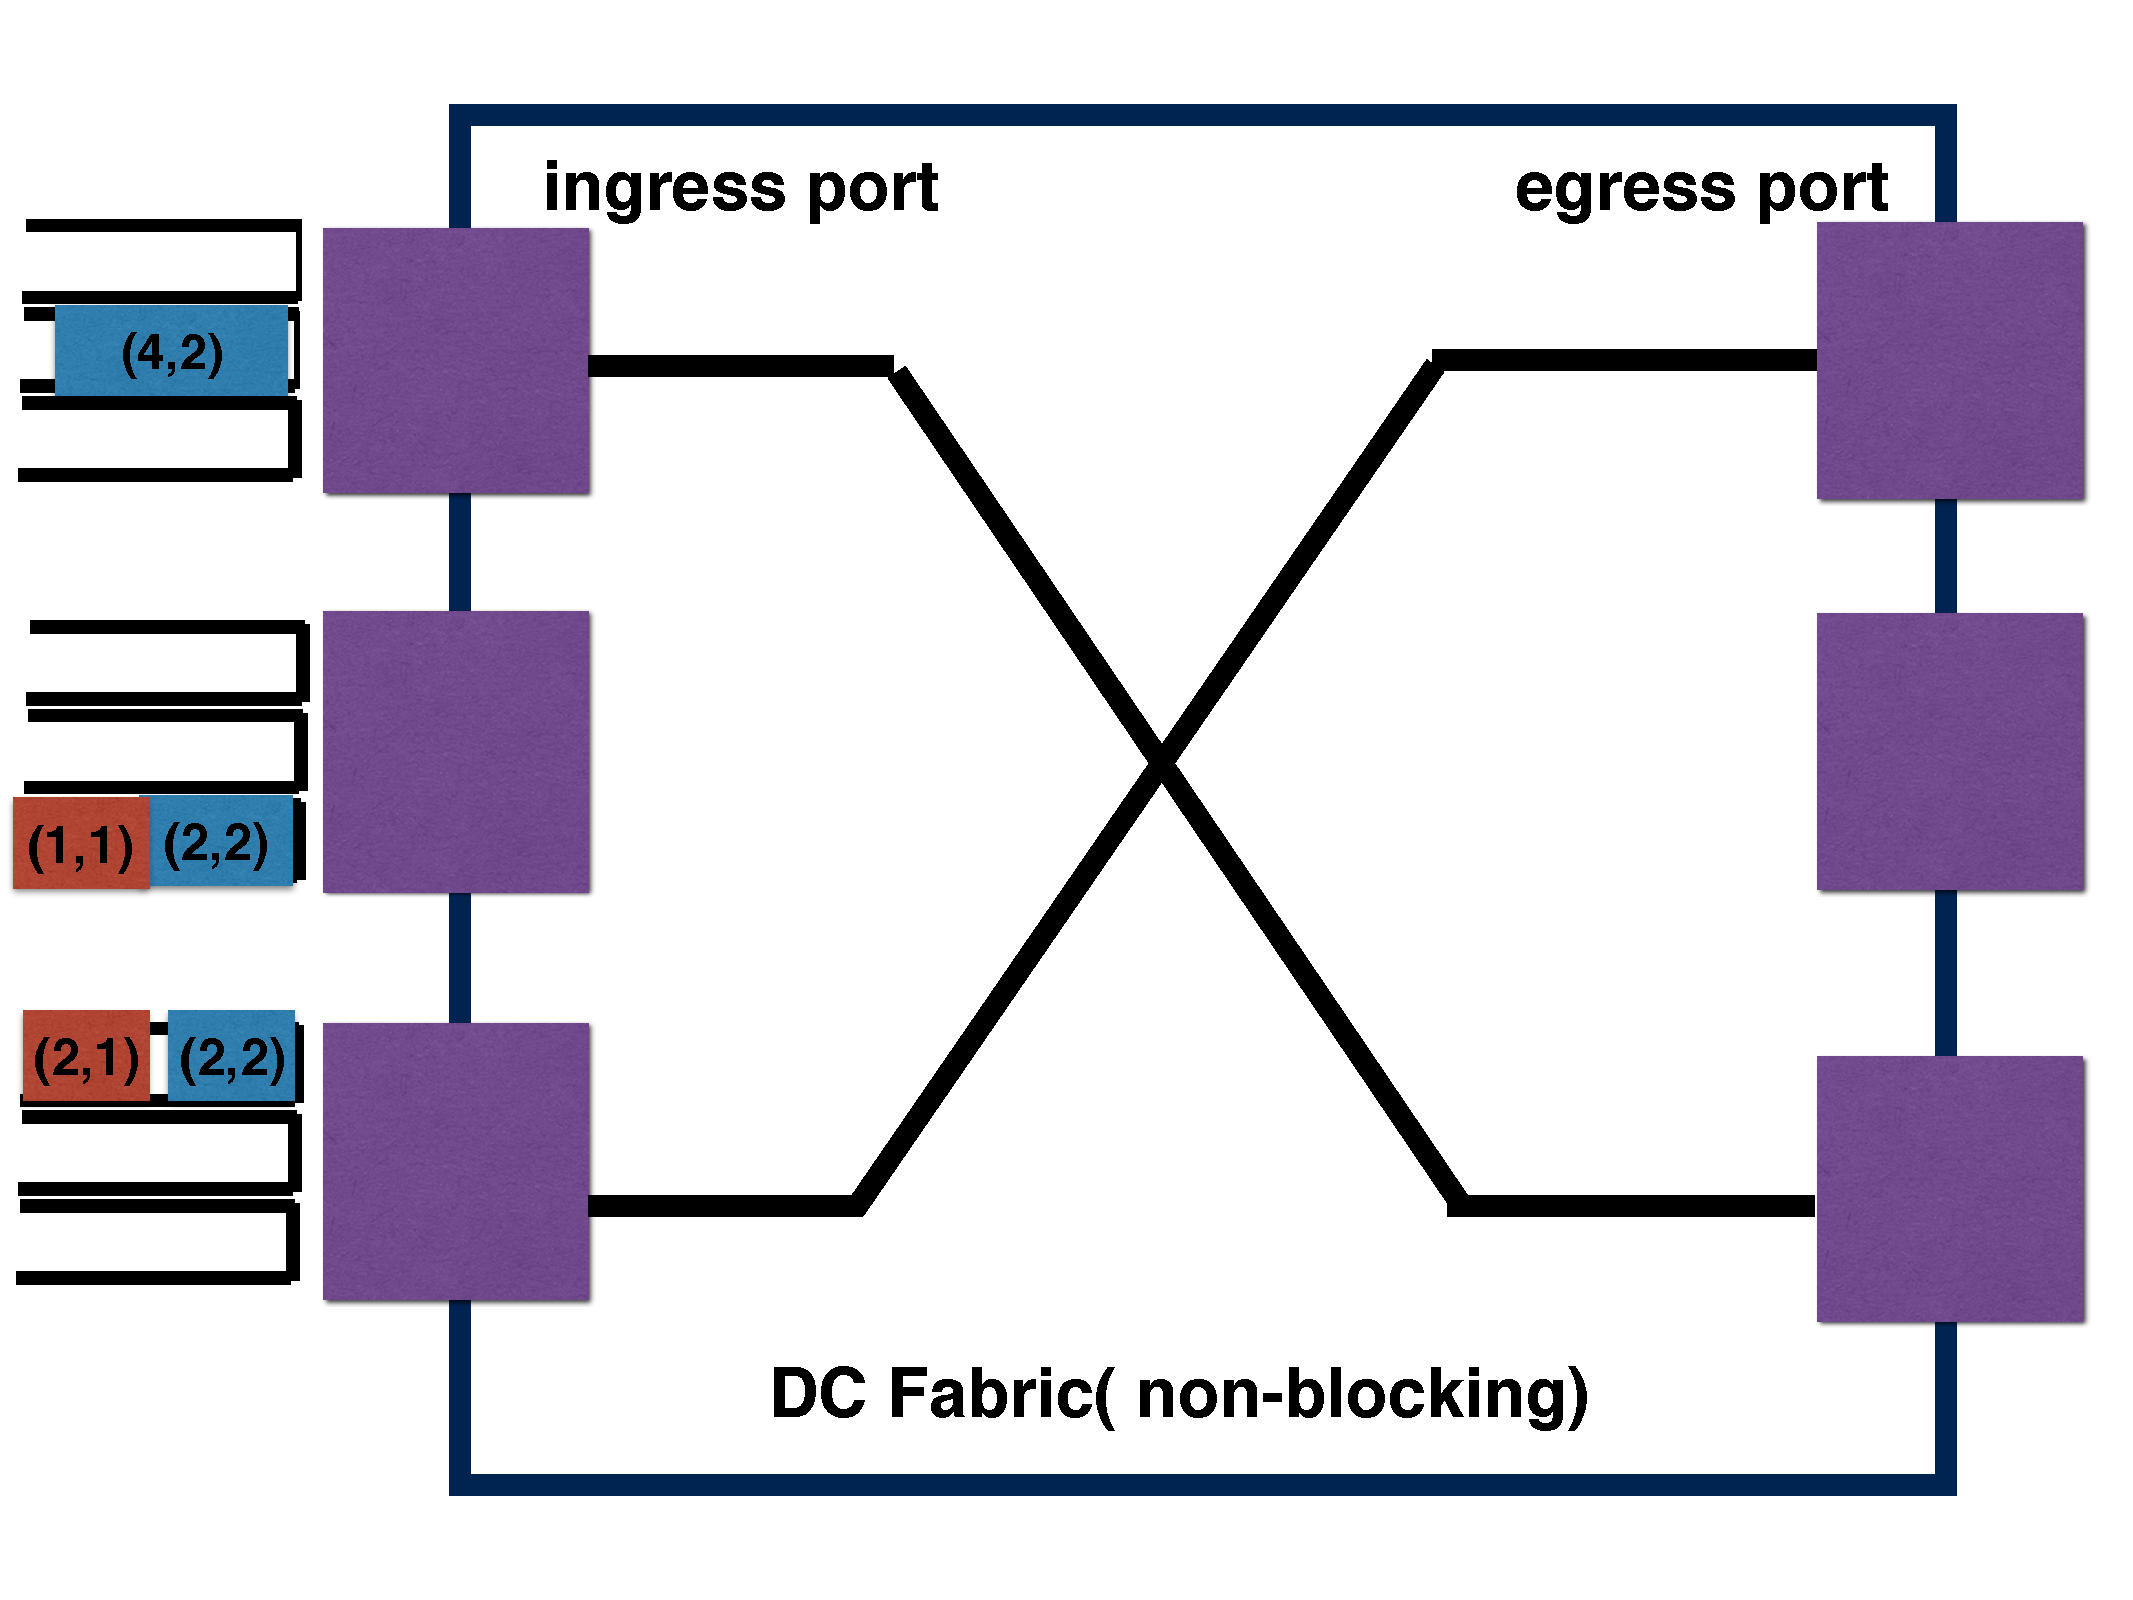
\includegraphics [width=0.8\columnwidth] {./figs/background/non_blcoking.pdf}
%\caption{Data center as non-blocking fabric: in this fabric, congestion only occurs at the ingress ports or egress ports}
%\label{Datacenter-nonblocking-fig}
%\end{center}
%\end{figure}


Recent researches\cite{chowdhury2015efficient}\cite{huang2016sunflow}\cite{chowdhury2014efficient}\cite{pFabric}  
regard a data center network as  a big giant non-blocking switch which interconnects all machines.
In this mode, all machines' ports have the same normalized unit capacity, and flows compete bandwidth only at these ports, i.e., the ingress and egress ports of the big fabric.
Such an abstraction is reasonable and matches with the full bisection bandwidth topologies widely used in productional data centers, e.g., the non-blocking Clos topology .
In this paper, we use this model and assume congestions occur only at the ingress and egress ports.
%
%\subsection{Why we choose weight}
%Applications in data center have to contend with each others for limited network resources.
%The state-of-art schedule methods use coflows as the abstraction to capture the communication patterns in a rich set of data parallel applications,
%so that their application-level semantics can be effectively modeled.
%However, applications in data center have different level of emergence, 
%scheduling just depends on network condition as well as the physical property of coflows is not enough.
%We have to differentiate applications to satisfy their demands for bandwidth.
%
%Some previous study\cite{D2TCP}\cite{D3}\cite{zhang2015more} use deadline to express the emergency of applications,
%applications have different deadlines, thus bandwidth.
%However, in reality, many applications just have different importance and do not have to finish before particular time points,
%so that we abandon deadline to present the emergence of applications.
%In this paper, we use weight to express the emergence of applications.
%For the example supporting the internal communication requirement of a search engine with intense internal computation should be more emergent than supporting the file backup on a distributed storage system. 
%When scheduling coflows from these two applications, we would like to take this difference into consideration and assign different weights to them, i.e., coflows of search engine have a higher weight, while coflows of file back have a lower weight.
%In this case, instead of minimizing average coflow completion time, we try to minimize average weighted coflow completion time.

%\begin{table}[th!]\label{model_define}
%\begin{center}
%\tabcolsep=0.11cm
%\begin{tabular}{cc}
%\hline\hline \\[-0.7ex]
%{\bf Symbol} & {\bf Meaning} \\ 
%$N$& Number of servers, indexed by $i=1,\ldots,N$ \\
%$\psi$ & coflow, each coflow $\psi $ contains many flows\\
%$f_{\psi}^{j}$ & coflow $\psi$'s jth subflow \\
%$\Psi$ & coflow set, elements in this set are $\psi_1$,$\psi_2$,$\psi_3$..\\
%$C_{\psi}^{j}$ & the completion time of $f_{\psi}^{j}$ \\
%$C_{\psi}$ & the completion time of $\psi$ \\
%$P_{\psi}^{j_{in}}$ & ingress port for $f_{\psi}^{j}$\\
%$P_{\psi}^{j_{out}}$ & egress port for $f_{\psi}^{j}$\\
%$L_{\psi}$ & number of  flows in coflow  $\psi$ , indexed by   $i=1,\ldots,N$\\
%$R_{P} $ &\ remaining capacity for port P that is measured by the system\\
%
%$w_{\psi}$ & weight for task $\psi$ \\
%$p_{\psi}^j$ & transfer time for flow  $f_{\psi}^{j}$ \\
%$d_{\psi}^j$ & volume for flow  $f_{\psi}^{j}$ \\
%$r_{\psi}^{j}$ & start (release) time of flow  $f_{\psi}^{j}$ \\
%
%\hline\hline \\[0.5ex]
%\end{tabular} \caption{Main notation.}
%\end{center}
%%\vspace{-0.3in}
%\end{table}
%\vspace{-.1in}


\subsection{Problem Formulation and Hardness Proof}

We consider the scheduling of $n$ coflows in a data center network modeled as a non-blocking fabric with $m$ hosts, i.e., there are $m$ ingresses and $ m$ egresses.
A coflow is a collection of flows sharing a common performance goal, e.g., minimizing the completion time of the latest flow or ensuring that flows meet a common deadline, and is denoted by $F^{(k)}=\{f^k_{i,j}|1 \leq i\leq m,1\leq j \leq m\}$, where $k$ is the sequence number assigned to the coflow, and $f^k_{i,j}$ is the normalized size of the flow (in this coflow $F^{(k)}$) sent from host $i$ to host $j$. Since every port has a unit capacity, the transfer time of the flow (i.e., the time the flow actually occupies the port) $f^k_{i,j}$ is also $f^k_{i,j}$.
If there is no flow from host $i$ to host $j$, then $f^k_{i,j}=0$. In the present, we simply assume all flows arrive at the same time, but we will remove this assumption when designing the online scheduling algorithm in the next section.
We use  $w_k$ to denote the weight, i.e., the emergence, of each coflow $F^{(k)}$, so that its completion time $C_k$ can be optimized with regard to its weight. Then the Idealized Weighted Coflow Completion Time Minimization (IWCCTM) problem is defined as follows:

\begin{eqnarray}
& {\rm minimize} & \sum_{k=1}^{n} w_{k} C_{k} \label{eq:WCCO-SC} \\
& {\rm s.t.} &\forall k,j:  \sum_{\forall l:C_l \leq C_k}\sum_{i=1}^{m}f_{i,j}^{(l)} \leq C_k  \label{eq:ingress_constraint}\\
&&\forall k,i: \sum_{\forall l:C_l \leq C_k}\sum_{j=1}^{m}f_{i,j}^{(l)} \leq C_k   \label{eq:egress_constraint}
\end{eqnarray}

Our goal is to minimize the sum of the weighted coflow completion times.
The constraints (\ref{eq:ingress_constraint}) and (\ref{eq:egress_constraint}) are due to the competition on the capacity of each port. 
For a coflow $F^{(k)}$ with completion time $C_k$, consider the set of coflows that finish before it, i.e., $F^{(l)}$: $C_l \le C_k$. For any ingress port $i$ (or egress port $j$), the total flow transfer time of this coflow on this port is at least $\sum_{j=1}^{m}f_{i,j}$ (or $\sum_{i=1}^{m}f_{i,j}$, correspondingly), which must be no greater than $C_k$. 

Consider a simplified version of this problem, where we want to minimize the total completion time of flows competing a single link. It is well known that {\em shortest job first} is the optimal non-preemptive scheduling policy, while {\em short remaining time first} is the optimal preemptive one. However, our problem for scheduling weighted coflows over multiple links is much harder, as indicated by the following proposition
\begin{proposition} \label{WCCO-eq}
If only non-preemptive scheduling is allowed, the IWCCTM problem is equivalent to the problem of minimizing the sum of weighted completion times in a concurrent open shop \cite{mastrolilli2010minimizing} and it is NP-hard.
\end{proposition}

\begin{IEEEproof}
The concurrent open shop problem \cite{mastrolilli2010minimizing} can be described as a set of machines $M = \{1,...,m\}$, with each machine capable of processing one operation type. A  set of jobs $N = \{1,...,n\}$, with each job requiring specific quantities of processing for each of its $m$ operation types. 
Each job $j \in N$  has a weight $w_j \in R > 0$, and the processing time of job $j$'s operation on machine $i$ is $p_{ij} \in R\ge0$. 
A job is completed when all its operations are completed. In particular, operations from the same job can be processed in parallel. 


  %we mark ingress ports as $1..m$ and egress ports as $ m+1...2m$.
%We consider the transferring time of coflow $F^{(k)}$ through port p ($1\leq p \leq $2m):
%
%
%\begin{eqnarray} \label{load_define}
%T_p^{(k)}=\left\{ \begin{array}{ll}
%\sum_{j=1}^mf_{i,j}^{(k)}& \textrm{$1\leq p \leq $m}\\
%\sum_{i=1}^mf_{i,j}^{(k)} & \textrm{m$<p\leq$ 2m}
%\end{array} \right.
%\end{eqnarray}
For our $m \times m$ network fabric, a coflow $F^{(k)}$ has $2m$ transfer tasks ($m$ tasks on the ingress ports and $m$ on the egresses ports). 
Consider the concurrent open shop scheduling problem with $2m$  machines of the same capacity and  
$n$ jobs, where each job has $2m$ types of operations on the $2m$ machines. 
There is a one-to-one correspondence between a coflow and a job, and between one type of operation on a machine and one transfer task on a port. It has been proved that minimizing the average weighted job completion time is NP-hard  \cite{mastrolilli2010minimizing}\cite{chen2000supply}\cite{roemer2006note}\cite{qiu2016experimental}, so the IWCCTM problem is also NP-hard.
\end{IEEEproof}


%.  Assume there are N machines (indexed by 1,2,...N) connecting to the data center network. Each machine connects to the giant switch through the link with the capacity of R. We define the coflow set as $\Psi$ and each coflow contains many flows($f_{\psi}^{j}$) whose source ($P_{\psi}^{j_{in}}$ )and destination($P_{\psi}^{j_{out}}$ ) are known beforehand. The weight for coflow $\psi$ is $w_{\psi}$.
%$p_{\psi}^j$  is transfer time for flow  $f_{\psi}^{j}$, $r_{\psi}^{j}$ is the start (release) time of flow  $f_{\psi}^{j}$ and $d_{\psi}^j$ is volume for flow  $f_{\psi}^{j}$ .  Details for our model is shown at Table \ref{model_define}.

%We give the definition of Concurrent Open Shop problem, then we prove WCCO is equivalent.  The problem of concurrent open shop problem can be described as: considering that a job consists of up to m different components to be processed on a specific one of m dedicated machines. Components are independent of each other, such that components of the same job can be processed in parallel on different machines. A job is completed once all of its components are completed \cite{roemer2006note}. The goal of concurrent open shop problem is to try to find a 
%sequence to minimize weight completion time or to find a sequence to let more jobs finish before deadline\cite{chen2000supply}.

%\begin{proposition} \label{WCCO-eq}
%Minimizing weight completion time of coflows is equivalent to minimizing weight  completion time of jobs in concurrent open shop problem.
%\end{proposition}
%

%
%(\ref{load_define}) gets the larger loads of ingress port and egress port. For the single coflow situation, weight completion time of coflow $L(F^{(k)})$ can be computed as $w_k*L(F^{(k)})$.
%
%Secondly,  assume there are two coflows $F^{(k)}$ and $F^{(l)}$, The priority of coflows indicates the schedule sequence of them.
%Let  P(.) denote the priority of coflow and the schedule sequence of  $F^{(k)}$ and $F^{(l)}$ can be defined as  definition \ref{sequence_definition}.

%\begin{definition} \label{sequence_definition}
% For any two coflows  $F^{(k)}$ and $F^{(l)}$, $P(F^{(k)}) \prec P(F^{(l)})$ means coflow  $P(F^{(k)})$ has lower priority value than $P(F^{(l)})$ and scheduler should schedule $F^{(k)}$ before $F^{(l)}$. $P(F^{(k)}) \succ P(F^{(l)})$ means coflow  $P(F^{(k)})$ has higher priority value than $P(F^{(l)})$ and scheduler should schedule $F^{(k)}$ after $F^{(l)}$.
%\end{definition}
%
%For two coflows, we can define the operation adding of them as follows:
%\begin{definition} \label{add_definition}
% For any two coflows  $F^{(k)}$ and $F^{(l)}$. We can define the single new  $m \times m $ coflow $F^{(n)}= F^{(k)} \bigcup F^{(l)}$, whose flow demand $f^n_{i,j}=f^k_{i,j}+f^l_{i,j}$.
% \end{definition}
% 
% 
% \begin{lemma} \label{two-coflow}
%For the two coflows, say $F^{(k)}$ and $F^{(l)}$, the optimum of $\mathbb{\min \max} \{C_l,C_k\}$ is $L( F^{(k)} \bigcup F^{(l)})$
%\end{lemma}
%\begin{IEEEproof}
%Firstly, For the single coflow n, its optimal completion time $L(F^{(n)})$ . Then we prove that $L( F^{(k)} \bigcup F^{(l)})$ is the low bound of
%$\mathbb{\min \max} \{C_l,C_k\}$. It is obvious that   $\mathbb{\max}\{C_l,C_k\} \ge L( F^{(k)} \bigcup F^{(l)})$. This is because if $\mathbb{\max}\{C_l,C_k\} < L( F^{(k)} \bigcup F^{(l)})$, then
%both $F^{(k)}$ and $F^{(l)}$ can finish before $L( F^{(k)} \bigcup F^{(l)})$. According to Definition \ref{add_definition}, $L( F^{(k)} \bigcup F^{(l)})=L(F^{(n)})$, so coflow  $F^{(n)}$ can finish before 
%$L( F^{(n)})$. This is contradict to the optimal completion time of $F^{(n)}$ is $L(F^{(n)})$.
%\end{IEEEproof}
%
%Lemma \ref{two-coflow} indicates that for two coflow system, $F^{(k)}$ and $F^{(l)}$, the optimal schedule completion time of the latter one is $L( F^{(k)} \bigcup F^{(l)})$. Then for weight completion time $\min\{w_l*C_l+w_k*C_k\}$, if $P(F^{(k)}) \prec P(F^{(l)})$, the optimal value of $\min\{w_l*C_l+w_k*C_k\}$ is $w_k*L(F^{(k)})+w_l*L( F^{(k)} \bigcup F^{(l)})$. Else if $P(F^{(k)}) \succ P(F^{(l)})$, the optimal value of $\min\{w_l*C_l+w_k*C_k\}$ is $w_l*L(F^{(l)})+w_k*L( F^{(k)} \bigcup F^{(l)})$.
%
%Thirdly, we generate this conclusion to coflow set. Assume there are g coflows.  Let $\gamma(k)$ denote the priority sequence of coflow k.  $WT(\gamma)$ denote the weight completion time under priority permutation $\gamma$:
%
%\begin{eqnarray} \label{weight_completion_gamma}
%WT(\gamma)= \sum_{i=1}^gw_i*L(\sum_{j=1}^i F^{(\gamma|j)})
%\end{eqnarray}

%So, Minimizing the weight coflow completion  for a given set of coflows is equivalent to finding a permutation  $\gamma$ for them (i.e., optimal priority permutation), so that WT is minimized. so far, we have changed the problem of minimizing coflow weight completion time has been changed to finding the optimal order permutation for them, which is quite similar to concurrent open shop problem. They are equivalent indeed. Next, we will describe the equivalence of them. 
%
%For each coflow $F^{(k)}$, let $f_i^{k}=\sum_{j=1}^mf_{i,j}^{k}$, for ingress ports i=1,2...m and  $f_{j+m}^{k}=\sum_{i=1}^mf_{i,j}^{k}$ for egress ports j=1,2...,m. Substitute $f_i^{k}$ and $f_{j+m}^{k}$ into (\ref{weight_completion_gamma}), then we get the fact that find the permutation of coflow is the same case as finding the optimal sequence for minimizing weight job completion time in concurrent open shop problem. In the problem, there are 2m jobs donated as $f_i^{k}$ and $f_{j+m}^{k}$ to be performed on 2m machines.  The machine index is denoted as i=1,2,..2m. On the contrary, by letting flows deriving from the same ingress port drain by the same egress port, we can construct concurrent open shop problem's corresponding coflow schedule problem.
%
%Now, we have proved proposition \ref{WCCO-eq} which is the equivalence of minimizing coflow weight completion time and minimizing job weight completion in concurrent open shop problem.
%According to \cite{roemer2006note} and \cite{mastrolilli2010minimizing}, finding a sequence of minimizing weight job completion time is NP-hard. As the problem is equivalent to minimizing coflow weight completion time, so finding a permutation of coflow to minimize weight coflow completion time is also NP-hard.


\section{Algorithms and System Design}\label{algorithm}
In this section, we first propose for the IWCCTM problem a non-preemptive scheduling algorithm that is 2-approximate optimal, following the idea presented in [24]. Then we remove the assumption that all coflows arrive at the same time and flow sizes are known a priori, and derive an information-agnostic preemptive scheduling algorithm that can work in an online fashion. Based on this latter algorithm, we further introduce a scheduling system named Yosemite. Yosemite relies on the Akka [2] and kryo [3] libraries, and can readily be deployed in a productional cloud environment like openstack.
 
\subsection{Non-preemptive Scheduling Algorithm for IWCCTM}
For minimizing the average weighted job completion time in the concurrent open shop problem, the best known theoretical result is a 2-approximation greedy algorithm\cite{kumar2011lp}\cite{mastrolilli2010minimizing}. Since our IWCCTM problem has a close relationship with it, we can derive a similar 2-approximate non-preemptive scheduler for IWCCTM, as shown in Algorithm \ref{offline}.
 \begin{algorithm} 
 \caption{2-approximate Non-preemptive Scheduling Algorithm for IWCCTM}
 \begin{algorithmic}[1]\label{offline}
 \renewcommand{\algorithmicrequire}{\textbf{Input:}}
 \renewcommand{\algorithmicensure}{\textbf{Output:}}
  \REQUIRE  Coflow list $\mathcal{F}=\{F^{(k)}\}$, weight list $\mathcal{W}=\{w_k\}$, $1 \le k \le n$;  
 %flow size $f_{i,j}$ from port i to port j, where $1 \leqslant i\leqslant m$,$1 \leqslant j \leqslant m$
  \ENSURE  a permutation $\gamma$ of $\{1, \dots, n\}$;
  \STATE $\mathcal{P} \gets \{1, \dots, 2m\}$, $\mathcal{R} \gets \{1, \dots, n\}$
%  \STATE $\gamma:\{1,2,...n\} \gets \mathcal{C}$
%  \\ \textit{$UC\gets\{1,2,3...n\}$}
%  \\ \textit{$P\gets\{1,2,3...2m\}$}
%  \\ \textit{$W\{1,2,...n\}\gets\{w_1,w_2,w_3...w_n\}$}
  \STATE $L_i^{(k)}= \sum_{j=1}^mf_{i,j}^{(k)}$  for $1 \le k \le n$ and $i \le m$
  \STATE $L_{j+m}^{(k)}= \sum_{i=1}^mf_{i,j}^{(k)}$ for $1 \le k \le n$ and $ j \le m$
  \STATE $L_p=\sum_{1 \le k \le n}L_p^{(k)}$ for each $p \in \mathcal{P}$
  \FOR{$i$ from $n$ to $1$ }
    \STATE $p^*=\arg \max \limits_{p \in \mathcal{P}}L_p$
    \STATE $\gamma[i]=r^*=\arg\min \limits_{r \in \mathcal{R}} w_r/L_{p^*}^{(r)}$
    \STATE $\theta=w_{r^*}/L_{p^*}^{(r^*)}$
    \STATE $\mathcal{R} = \mathcal{R} \setminus \{r^*\}$
    \STATE $w_r = w_r-\theta \times L_{p^*}^{(r)}$ for all $r \in \mathcal{R}$
    \STATE $L_p=L_p-L_p^{(r^*)}$ for all $p \in \mathcal{P}$
  \ENDFOR
 \end{algorithmic} 
 \end{algorithm}
 
Algorithm \ref{offline} takes a list $\mathcal{F}$ of $n$ coflows and a list $\mathcal{W}$ of $n$ weights as its input, where the $k$-th coflow in $\mathcal{F}$ is defined as $F^{(k)}=\{f^k_{i,j}|1 \leq i\leq m,1\leq j \leq m\}$, whose weight is $w_k$, the $k$-th weight in $\mathcal{W}$, as already explained in Sec \ref{system model}.
%and $f_{i,j}$, where $\mathcal{C}$ $f_{i,j}^k$ is the volume of data sent from port i to j. 
It outputs $\gamma$, a permutation of $\{1, \dots, n\}$ that indicates the scheduling order of the $n$ coflows.

The Algorithm first composes a port list $\mathcal{P}=\{1, \dots, 2m\}$, corresponding to $m$ ingress and $m$ egress ports, and computes the total load on each port (line 1 $\sim$ 4). Then its iteratively finds the coflow to be scheduled in the $i$-th round, nonetheless in a reverse order. In each iteration, it finds the port ($p^*$) with the heaviest load, chooses the coflow who has the minimal ratio of coflow weight to its load on that port, and saves its index ($r^*$) in $\gamma[i]$ (line 6 $\sim$ 7). It then updates the set of coflows remaining to be scheduled as well as their weights, and the port load (line 8 $\sim$ 11), before it goes to the next iteration.

Algorithm \ref{offline} generates the permutation $\gamma$ as the scheduling order within $O(n(m+n))$ operations and is 2-approximate optimal. However, since IWCCTM makes some idealized assumptions, the algorithm cannot be straightforwardly used in real environment.
%\begin{figure}
 %\vspace{-8mm}
  %  \begin{minipage}{.47 \textwidth}
   %  % \begin{algorithm}[5]
   %     \caption{Minimize coflow completion time offline algorithm}
%        \label{alg:coflow_offline}
%        %\begin{algorithmic}
        %\STATE \textbf{for } every port :
        %\STATE \hspace{\algorithmicindent}  \textbf{for } every task $\psi$:
       %  \STATE \hspace{\algorithmicindent} \hspace{\algorithmicindent} \textbf{for} f in  $\psi$:
    %      \STATE \hspace{\algorithmicindent} \hspace{\algorithmicindent}\hspace{\algorithmicindent}  \textbf{if} f goes through port P:
 %          \STATE \hspace{\algorithmicindent} \hspace{\algorithmicindent}\hspace{\algorithmicindent}\hspace{\algorithmicindent} load[port]+=p[$\psi$][f]
%\STATE k=n
%\STATE\textbf{while} $k>1:$
%\STATE\hspace{\algorithmicindent} u=$\max \limits_{i \in N}load[i]$
%\STATE Compute current objective value $B^{(0)}$
%\STATE \textbf{do}
%\STATE \hspace{\algorithmicindent} Solve Convex Problem { Prob\_Z} to get $z_{i,t}$ for given $\pi_{i,j,t}$ for all $i$
%\STATE \hspace{\algorithmicindent} Set $k_{L,i,t}=0$, $k_{U,i,t} = k_i$
%\STATE \hspace{\algorithmicindent}\textbf{do}
%\STATE \hspace{\algorithmicindent} \hspace{\algorithmicindent} Solve Convex Problem Prob\_$\Pi$ to get $\pi_{i,j,t}$ for given $z_{i,t}, \  k_{L,i,t}, \  k_{U,i,t}$ for all $i,j$
%\STATE \hspace{\algorithmicindent} \hspace{\algorithmicindent} Let $i_1 = \arg\max$ (fractional part of $\sum_{j=1}^m \pi_{i,j,t}$)
%\STATE \hspace{\algorithmicindent} \hspace{\algorithmicindent}$k_{L,i_1,t}= k_{U,i_1,t} = ceil(\sum_{j=1}^m \pi_{i,j,t})$
%\STATE \hspace{\algorithmicindent} \textbf{while} $\sum_i frac(\sum_{j=1}^m \pi_{i,j,t})>0$
%\STATE \hspace{\algorithmicindent}Compute new objective value $B^{(c+1)}$,  Update  $c=c+1$
%\STATE {\bf while} $B^{(c)}-B^{(c-1)}>\epsilon$
        %\end{algorithmic}
      %\end{algorithm}
    %\end{minipage}
   % \vspace{-.25in}�
 % \end{figure}
  
  
 

%The main process of Yosemite is as follows: There are two main process on the sender
%the sending process and the 
%When a coflow arrives, the corresponding sender will
%send the information to the master. Senders send flow information to maters.
%every T time, all senders send corresponding flow information to the master.
%The master will collect the information of all coflows and use the online algorithm to compute the sequence of the coflow.
%Then the master will send the sequence to the senders. The senders use the sequence to decide the bandwidth of each flow and 
%send flows with the result of the computation.
%
%We combine centralized with distributed scheduling method in our system.  The master is the brain of our method, it summarizes the
%information from the endpoints. Each machine in data center has a slaver damon. The slaver generates coflow information and sends 
%the flow information to master. After the sequence computation, it then use its rate limiter to do rate control.
%
%Priority queue is used at the sender side to help do the scheduling problem. Just as Fig .\ref{queue-fig}  shown.  There are N queues at the sender side,
%each queue has a priority $w_j$.  The number of flows that queue j can accommodate is $E_j$. Note, the lowest queue can accommodate infinite number of
%flow in reality.   

%\begin{figure}[b]
%\begin{center}
%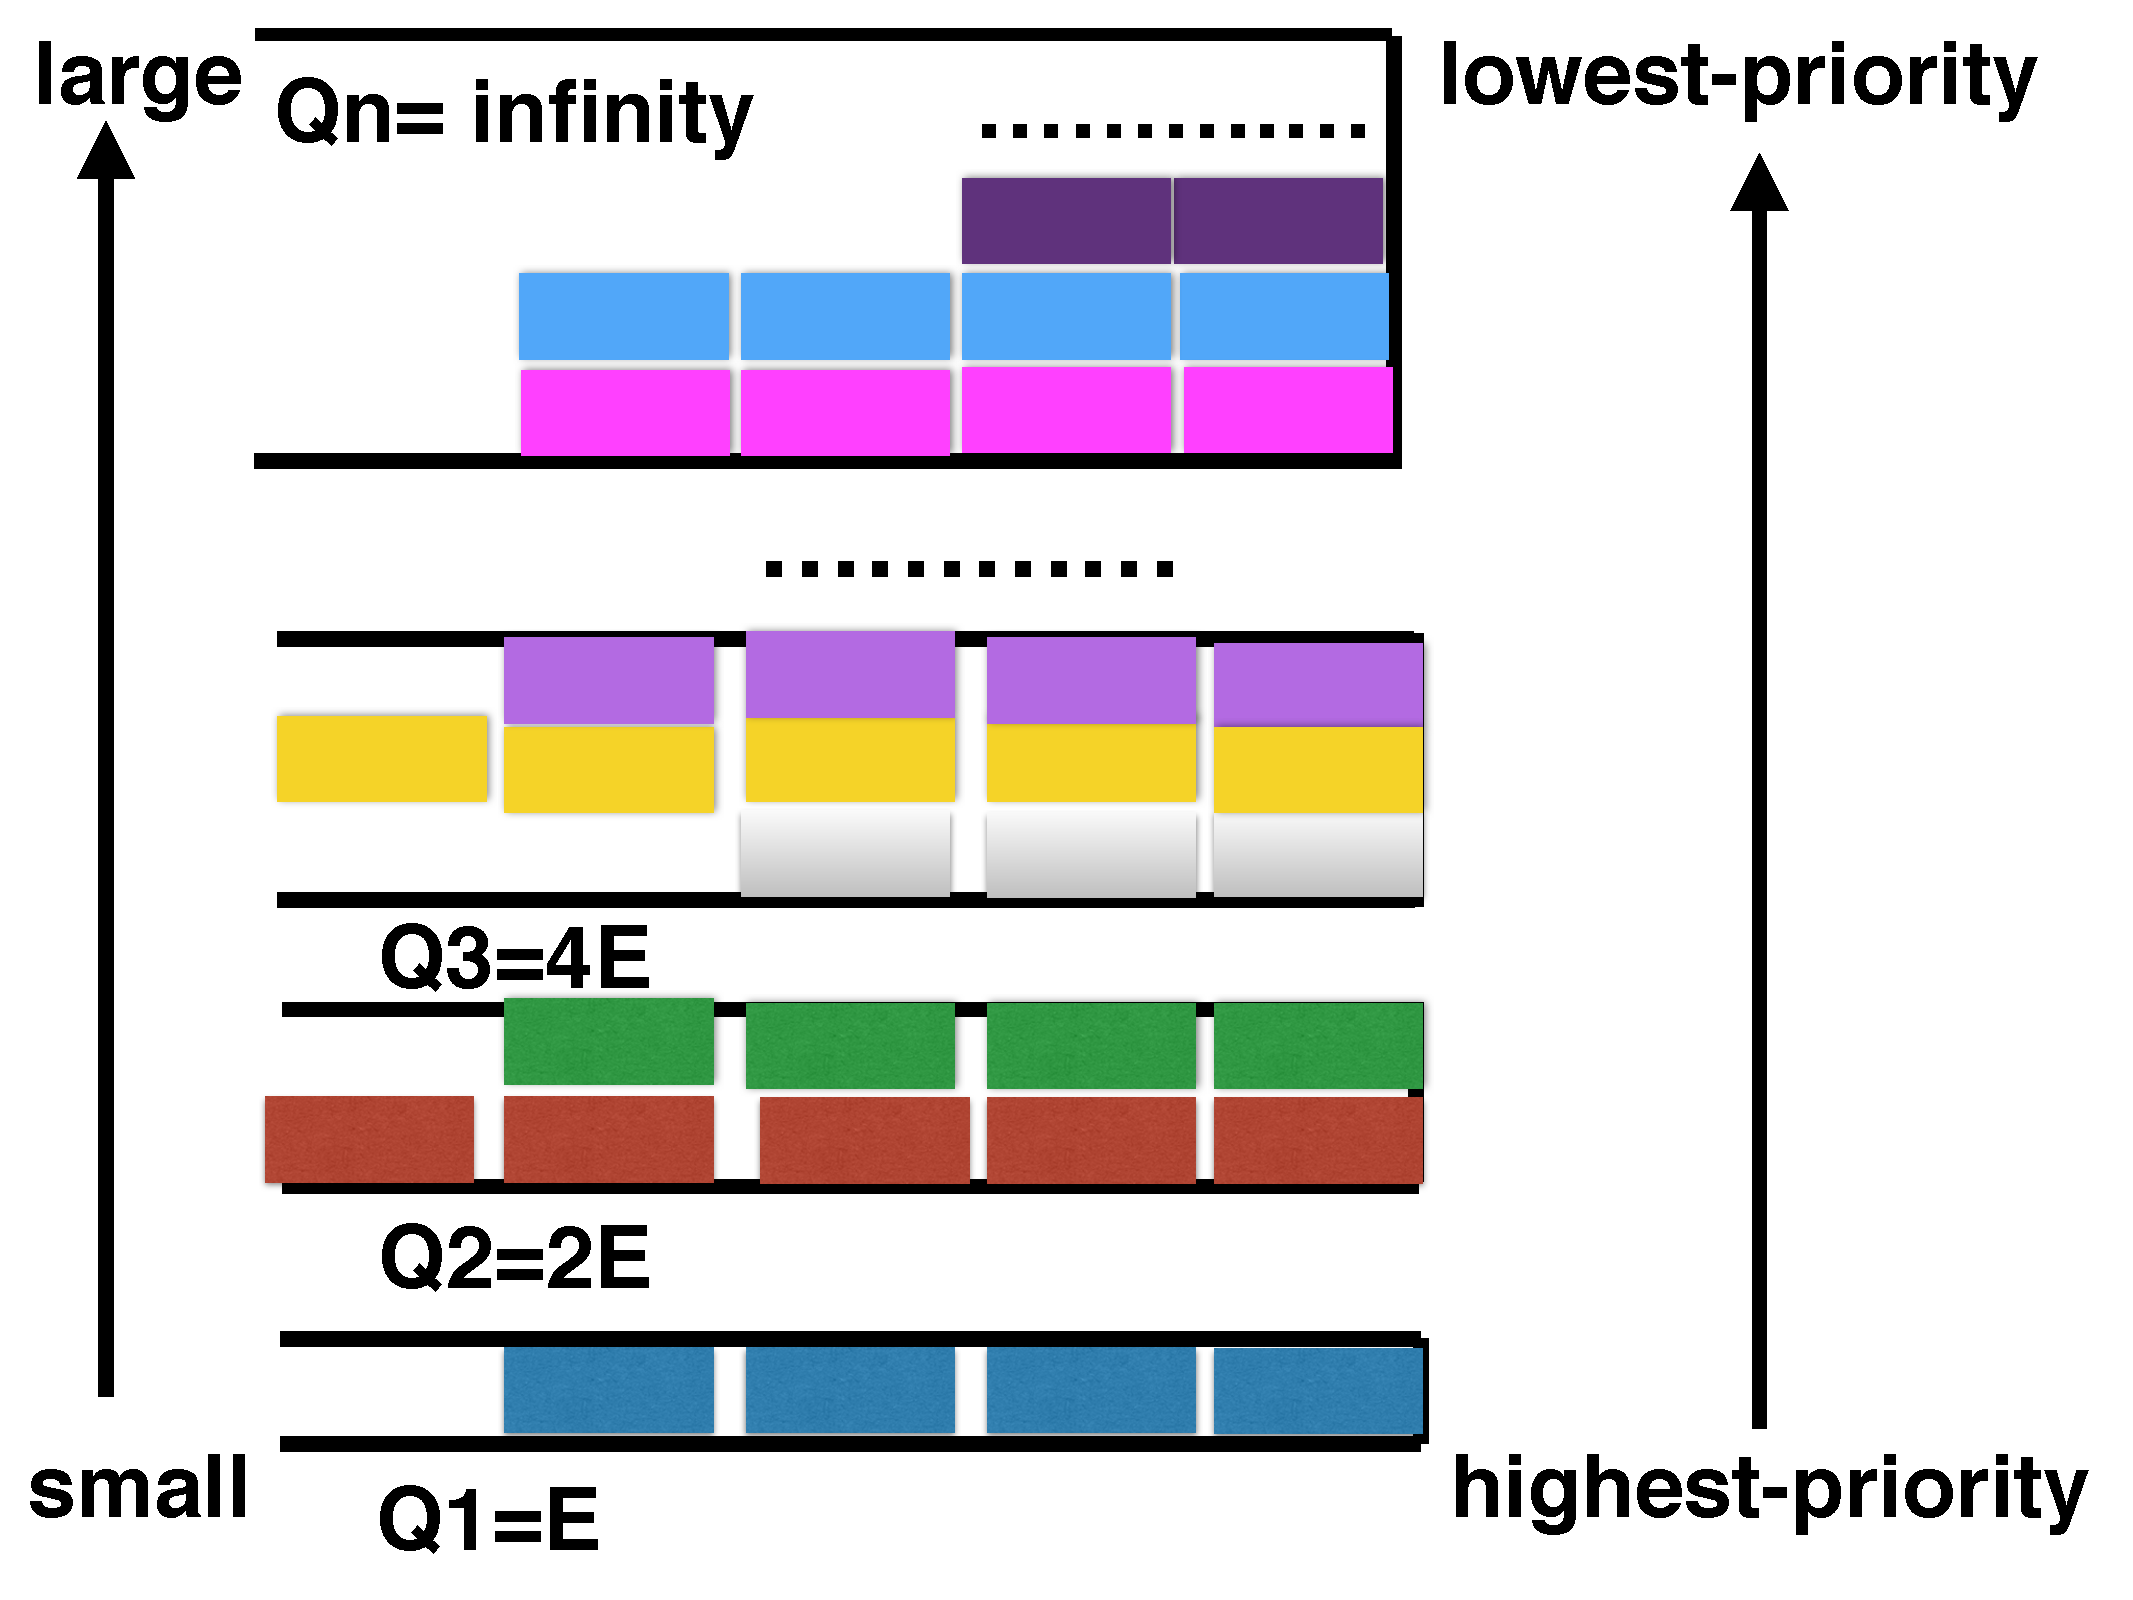
\includegraphics [width=0.8\columnwidth] {./figs/system/queue.pdf}
%\caption{Weight Priority Queue: from the bottom, the size of queue become larger and the priority lower }
%\label{queue-fig}
%\end{center}
%\end{figure}

%
%As the sequence of coflows is updated every T, however, in practice, some flows are always short and wait for T time may lead to bad performance.
%As a result, in our system, we set a threshold K,  flows whose size is smaller than K will get the lowest priority and this can avoid the condition of starvation.


\subsection{Information-agnostic Algorithm for minimizing WCCT}

IWCCTM assumes that flow sizes are known by the scheduler, and flows arrive a the same time. These idealized assumptions are unrealistic, so special care should be taken when we design a practical scheduler to be deployed in a real environment.

The key idea of Algorithm \ref{offline} lines in line 7 therein, where it tries to prioritize coflows with large weight but small load on the most loaded port $p^*$. In practice, ports in date center networks are expected to be load balanced by utilizing certain load-balancing techniques \cite{dean2008mapreduce}. We introduce a simplification that ignores the load difference on different ports, and just prioritize coflows with large weight but small load. By replacing the prioritizing rule in Algorithm \ref{offline} with this heuristic, we get a simple offline scheduling algorithm. This intermediate stage algorithm is for the sake of performance comparison and analysis only, so we omit its details due to space limitations. The computation of priorities in Algorithm \ref{offline} depends on the total load of each coflow, and we replace that with the volume of traffic it has sent. Since this volume can be measured cumulatively in realtime, the scheduler becomes flow information agnostic. This is particularly useful for scenarios where dynamic-sized flows are generated, for example, in hadoop or some other map-reduce style applications. After making all these changes, we process coflow arrivals, and derive Algorithm \ref{online-algorithm}. 
\if false
\begin{algorithm} 
 \caption{simple-offline approach to minimize average  weighted coflow completion time}
 \begin{algorithmic}[1]\label{simple-offline-algorithm}
 \renewcommand{\algorithmicrequire}{\textbf{Input: }}
 \renewcommand{\algorithmicensure}{\textbf{Output:}}
 \REQUIRE  Coflow set $\mathcal{C}$ ;  flow size $f_{i,j}$ from port i to port j, where $1 \leqslant i\leqslant m$,$1 \leqslant j \leqslant m$
  \ENSURE  $\gamma$
  \STATE $W\{1,2,...n\}\gets\{w_1,w_2,w_3...w_n\}$
  \STATE $L_i^{(k)}= \sum_{j=1}^mf_{i,j}^{(k)}$ for all k $\in$ $\mathcal{C}$ and i $\le$ m
   \STATE $L_{j+m}^{(k)}= \sum_{i=1}^mf_{i,j}^{(k)}$ for all k $\in$ $\mathcal{C}$ and j $\le$ m
    \STATE  $l^{(k)}$=$ \max \limits_{1 \le i \le 2m}L_i^{(k)}$ for all k $\in$$\mathcal{C}$
      \FOR{i $\in\{n,n-1,n-2...1\}$ }
     \STATE  $\gamma^{(i)}=\arg \max \limits_{k \in UC }\{\frac{1}{W[k]}\times \frac{1}{l^{(k)}}\}$
      \STATE $UC = UC \setminus\{\gamma[i]\}$
         \ENDFOR
     \end{algorithmic} 
 \end{algorithm}
 
Line4 of Algorithm \ref{simple-offline-algorithm} computes the transfer time for coflow, which means flow size should be known beforehand. 
However, in data centers, applications such as Hadoop can not know flow size beforehand and this constraints the usage of the method.
In this case, we use transferred size instead of flow size to compute the priority of coflow.
Coflows that have highest priority at first, but degrade with the increasing amount of data that are sent (\textbf{relaxation 2}).
Use this relaxation, we get the online Algorithm \ref{online-algorithm}.
\fi

 \begin{algorithm} 
 \caption{Information-agnostic Online scheduling to minimize WCCT}
 \begin{algorithmic}[1]\label{online-algorithm}
% \renewcommand{\algorithmicrequire}{\textbf{Input: }}
% \renewcommand{\algorithmicensure}{\textbf{Output:}}
% \REQUIRE  Coflow $F^{(k)}$ ;  $s_{i,j}^{(k)}$ that has been sent from port i to port j for Coflow $F^{(k)}$, where $1 \leqslant i\leqslant m$,$1 \leqslant j \leqslant m$
% \ENSURE  $\gamma$
  \IF{a new coflow arrives}
  \STATE update the coflow list $\mathcal{F}=\{F^{(k)}\}$
  \STATE $n=|\mathcal{F}|$
  \FOR{$1 \le k \le n$ } 
    \STATE update $s_{i,j}^{(k)}$, the cumulative volume of the traffic sent by coflow $F^{(k)}$, for $1 \le i, j \le m$
    \STATE $L_i^{(k)}= \sum_{j=1}^ms_{i,j}^{(k)}$ for $1 \le i \le m$
    \STATE $L_{j+m}^{(k)}= \sum_{i=1}^ms_{i,j}^{(k)}$ for $1 \le j \le m$
    \STATE $l^{(k)}$=$ \min \limits_{1 \le i \le 2m}L_i^{(k)}$
    \STATE $\alpha^{(k)}=l^{(k)}/w_k$
  \ENDFOR
  \STATE $\omega=$sort the list of $\{\alpha^{(k)}\}$ in nondecreasing order
  \STATE $\gamma=$index set of $\omega$
  \ENDIF
  \STATE initialize the bandwidth to be allocated on each ingress and egress port: $I_p=O_p=$ port physical bandwidth, for $1 \le p \le m$
  \FOR{$\ell$ from 1 to $n$}
    \STATE schedule coflow $F=F^{(\gamma[\ell])}$
    \STATE $r$ = min $\{I_p, O_q\}$, subject to $F$ still need to send traffic to port $p$ or receive traffic from port $q$
    \FOR{each unfinished flow $F_{i,j}$ in $F$} 
      \STATE allocate bandwith of $r$ to $F_{i,j}$
      \STATE update $I_i$ and $O_j$ by deducting $r$ from them 
    \ENDFOR
  \ENDFOR
  \STATE allocate remaining bandwidth equally to all unfinished flows
 \end{algorithmic} 
 \end{algorithm}


Algorithm \ref{online-algorithm} is called by a scheduler when a flow starts or finishes.
It prioritizes coflows according to the heuristics explained above (line 1 $\sim$ 13)\footnote{A coflow set $\mathcal{F}$ and the corresponding schedule order are maintained in the whole life of the scheduler, so that when an existing coflow starts or finishes a flow, the prioritization procedure is bypassed, and the schedule order remains unchanged.}, and allocates bandwidth to each flow (line 14 $\sim$ 22). At last, it distributes the unallocated bandwidth equally among all unfinished flows to provide resource conservation.
Algorithm \ref{online-algorithm}  is an information-agnostic online algorithm that dynamically schedule coflows according to their weights and the instantaneous network condition. Compared to the 2-approximate algorithm, it inevitably introduces some performane loss, but our evaluation shows there is only a small gap, as will be seen in Sec \ref{evaluation}.

% Similar to \cite{chowdhury2014efficient}, the load of each coflow is:
%
%\begin{eqnarray} \label{weight_completion_gamma}
%g^{(k)}=\max(\max \limits_i \frac{ \sum_{j=1}^mf_{i,j}^{(k)}}{Rem(P_i^{(in)})},\max \limits_j \frac{ \sum_{i=1}^mf_{i,j}^{(k)}}{Rem(P_j^{(out)})})
%\end{eqnarray}

%$Rem(P_i^{(in)})$ denotes the remaining port capacity of ingress port $P_i^{(in)}$. $Rem(P_j^{(out)})$ denotes the remaining port capacity of egress port $P_j^{(out)}$. 
%In our assumption, the capacity of each port is 1. 

%\subsection{Distance between the online and offline algorithm}
%In this section, we illustrate the distance between the online and the offline algorithm from the contents of algorithm and simulation.
%
%Let's first look at Algorithm \ref{offline}, Line 6 tries to find the bottleneck port and Line7 finds the slowest weighted coflow,
%so that result of the every for-loop in Algorithm \ref{offline} tries to find the slowest weighted coflow which owns the smallest priority.
%However, Algorithm\ref{online-algorithm} directly sets the coflow with the maximum weight and per-port load ratio with the highest priority.
%As a result, this can lead to some performance loss, 
%but in data center network, though assigning jobs with load balancing,
%load difference still exists in the ports, so that Algorithm\ref{online-algorithm} will have performance in practice.
%
%To see the performance loss between them, 
%we consider the schedule of 100 coflows served by a small-scale cluster consisting of 60 hosts in our simulator. 
%These hosts are connected with a non-blocking network fabric, where each port (both ingress and egress) has the capacity of 1 GB/s. 
%Details of the simulator can be seen at Section \ref{evaluation}. 
%Then we set coflows' arrival time to 0 and weight within 1 to 5, 
%and Fig. \ref{online-offline-fig} shows the result. 
%
%From Fig. \ref{online-offline-fig}, we can see the online algorithm performs close to the 2-approximate algorithms in total and only prolongs the transfer of large coflows. 
%As coflows are generated randomly, we repeat the numerical simulation 200 times. 
%Table \ref{tab:loss} shows the proportions of $\frac{avg \;wcct\  of \ online}{avg\; wcct \ of \  2-appr}-1$, where $avg\;wcct $ means average weighted coflow completion time.
%We can see that 64\% cases have less than 0.025 of performance loss.
%More than 91\% cases have less than 0.1 performance gap and no cases have more than 0.15 performance loss.  
%
%      \begin{table}[!htb]
%          \centering
%          \footnotesize
%          \caption{Performance loss result} \label{tab:loss}
%          \begin{tabulary}{\textwidth}{cccccr}
%              \toprule
%              $\leq 0\%$  & \multicolumn{1}{c}{$\leq 0.025$} & $\leq 0.05$& $\leq 0.1$ &$\leq 0.15$\\
%              \midrule
%              \multicolumn{1}{r}{0} & 64\%    &72\%    &91\%  &100\%  \\
%             \bottomrule
%          \end{tabulary}
%      \end{table}
%      
      
%\begin{table}[!htb]
%          \centering
%          \footnotesize
%          \caption{Comparison between the two algorithms} \label{tab:comparison}
%          \begin{tabulary}{\textwidth}{ccccr}
%              \toprule
%              \#Scheme  & \multicolumn{1}{c}{Sched-Mode} & Procedure & Performance \\
%              \midrule
%              \multicolumn{1}{r}{2-appr} & offline    & Complex     & High \\
%              \multicolumn{1}{r}{Yosemite} & online    & simple     & High \\
%              \bottomrule
%          \end{tabulary}
%      \end{table}
%      
%
%As Table. \ref{tab:comparison} shown, we conclude comparing with the offline algorithm, online algorithm has little performance loss. 
%Indeed, it is much more simple and can maintain relative high performance,
%so that in reality, using the online algorithm to schedule coflow is a good choice.

%\begin{figure}[b]
%\begin{center}
%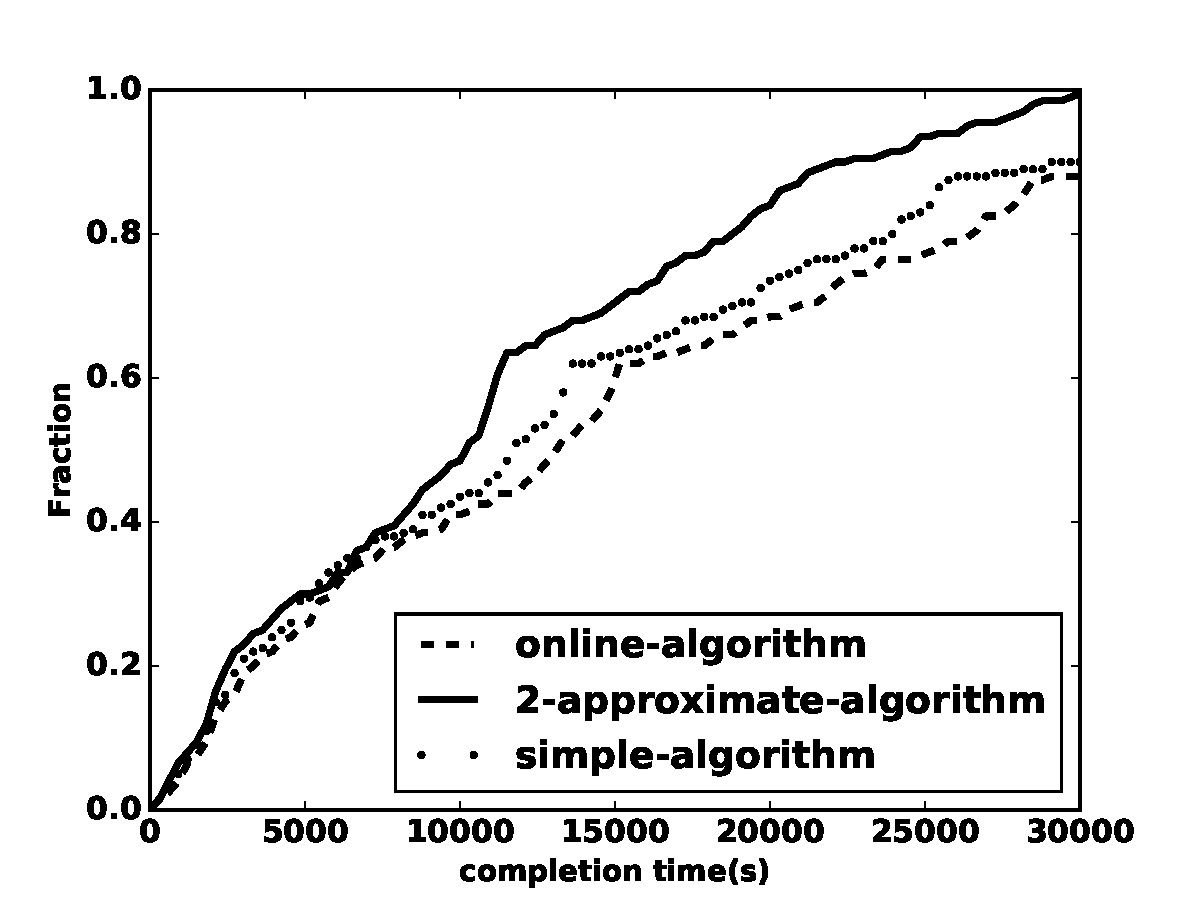
\includegraphics [width=0.6\columnwidth] {./figs/performance/online_offline.pdf}
%\caption{[Simulation] Performance comparison between 2-approximate algorithm and online algorithm}
%\label{online-offline-fig}
%\end{center}
%\end{figure}


\subsection{Yosemite System}

To make our scheduling algorithm practical, we design and implement a real scheduling system named Yosemite. Yosemite can be readily deployed in productional cloud environment like openstack. It employs the actor model\cite{actor}, uses Akka \cite{Akka} for message transferring, and uses kryo \cite{kryo} for object serialization. It consists of about 6000 lines of scala code, and can be downloaded at \cite{Yosemite}.

 \begin{figure}[b]
\begin{center}
%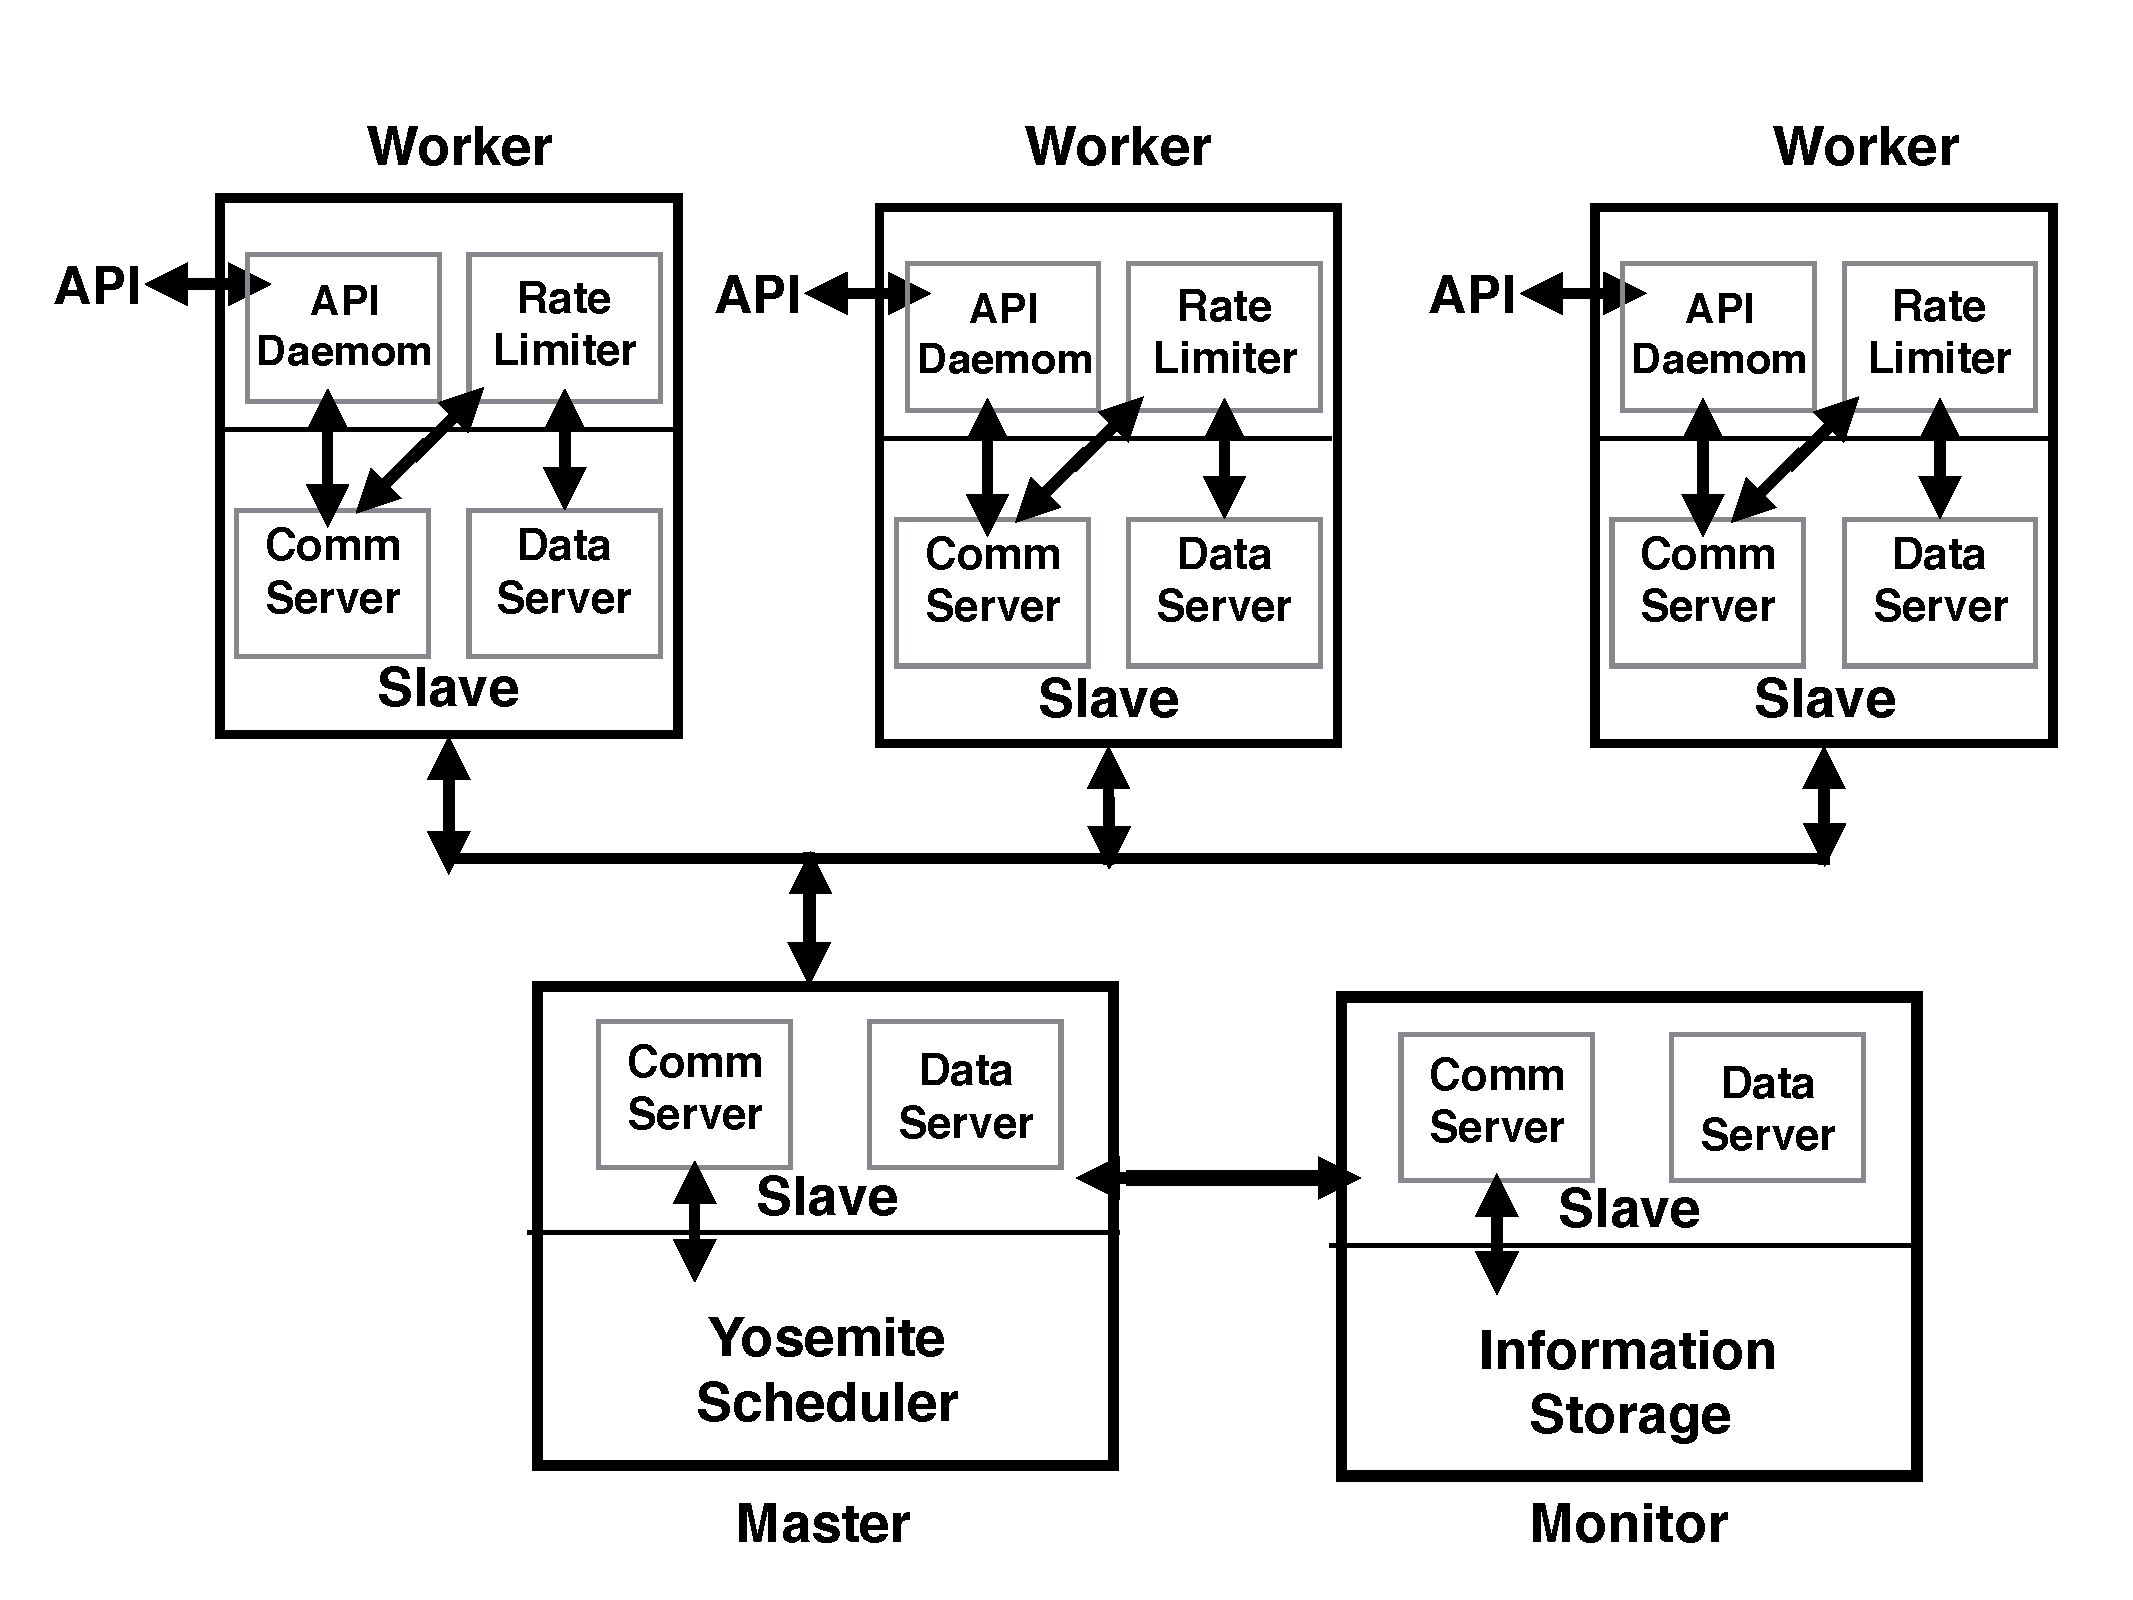
\includegraphics [width=0.6\columnwidth] {./figs/background/system.pdf}
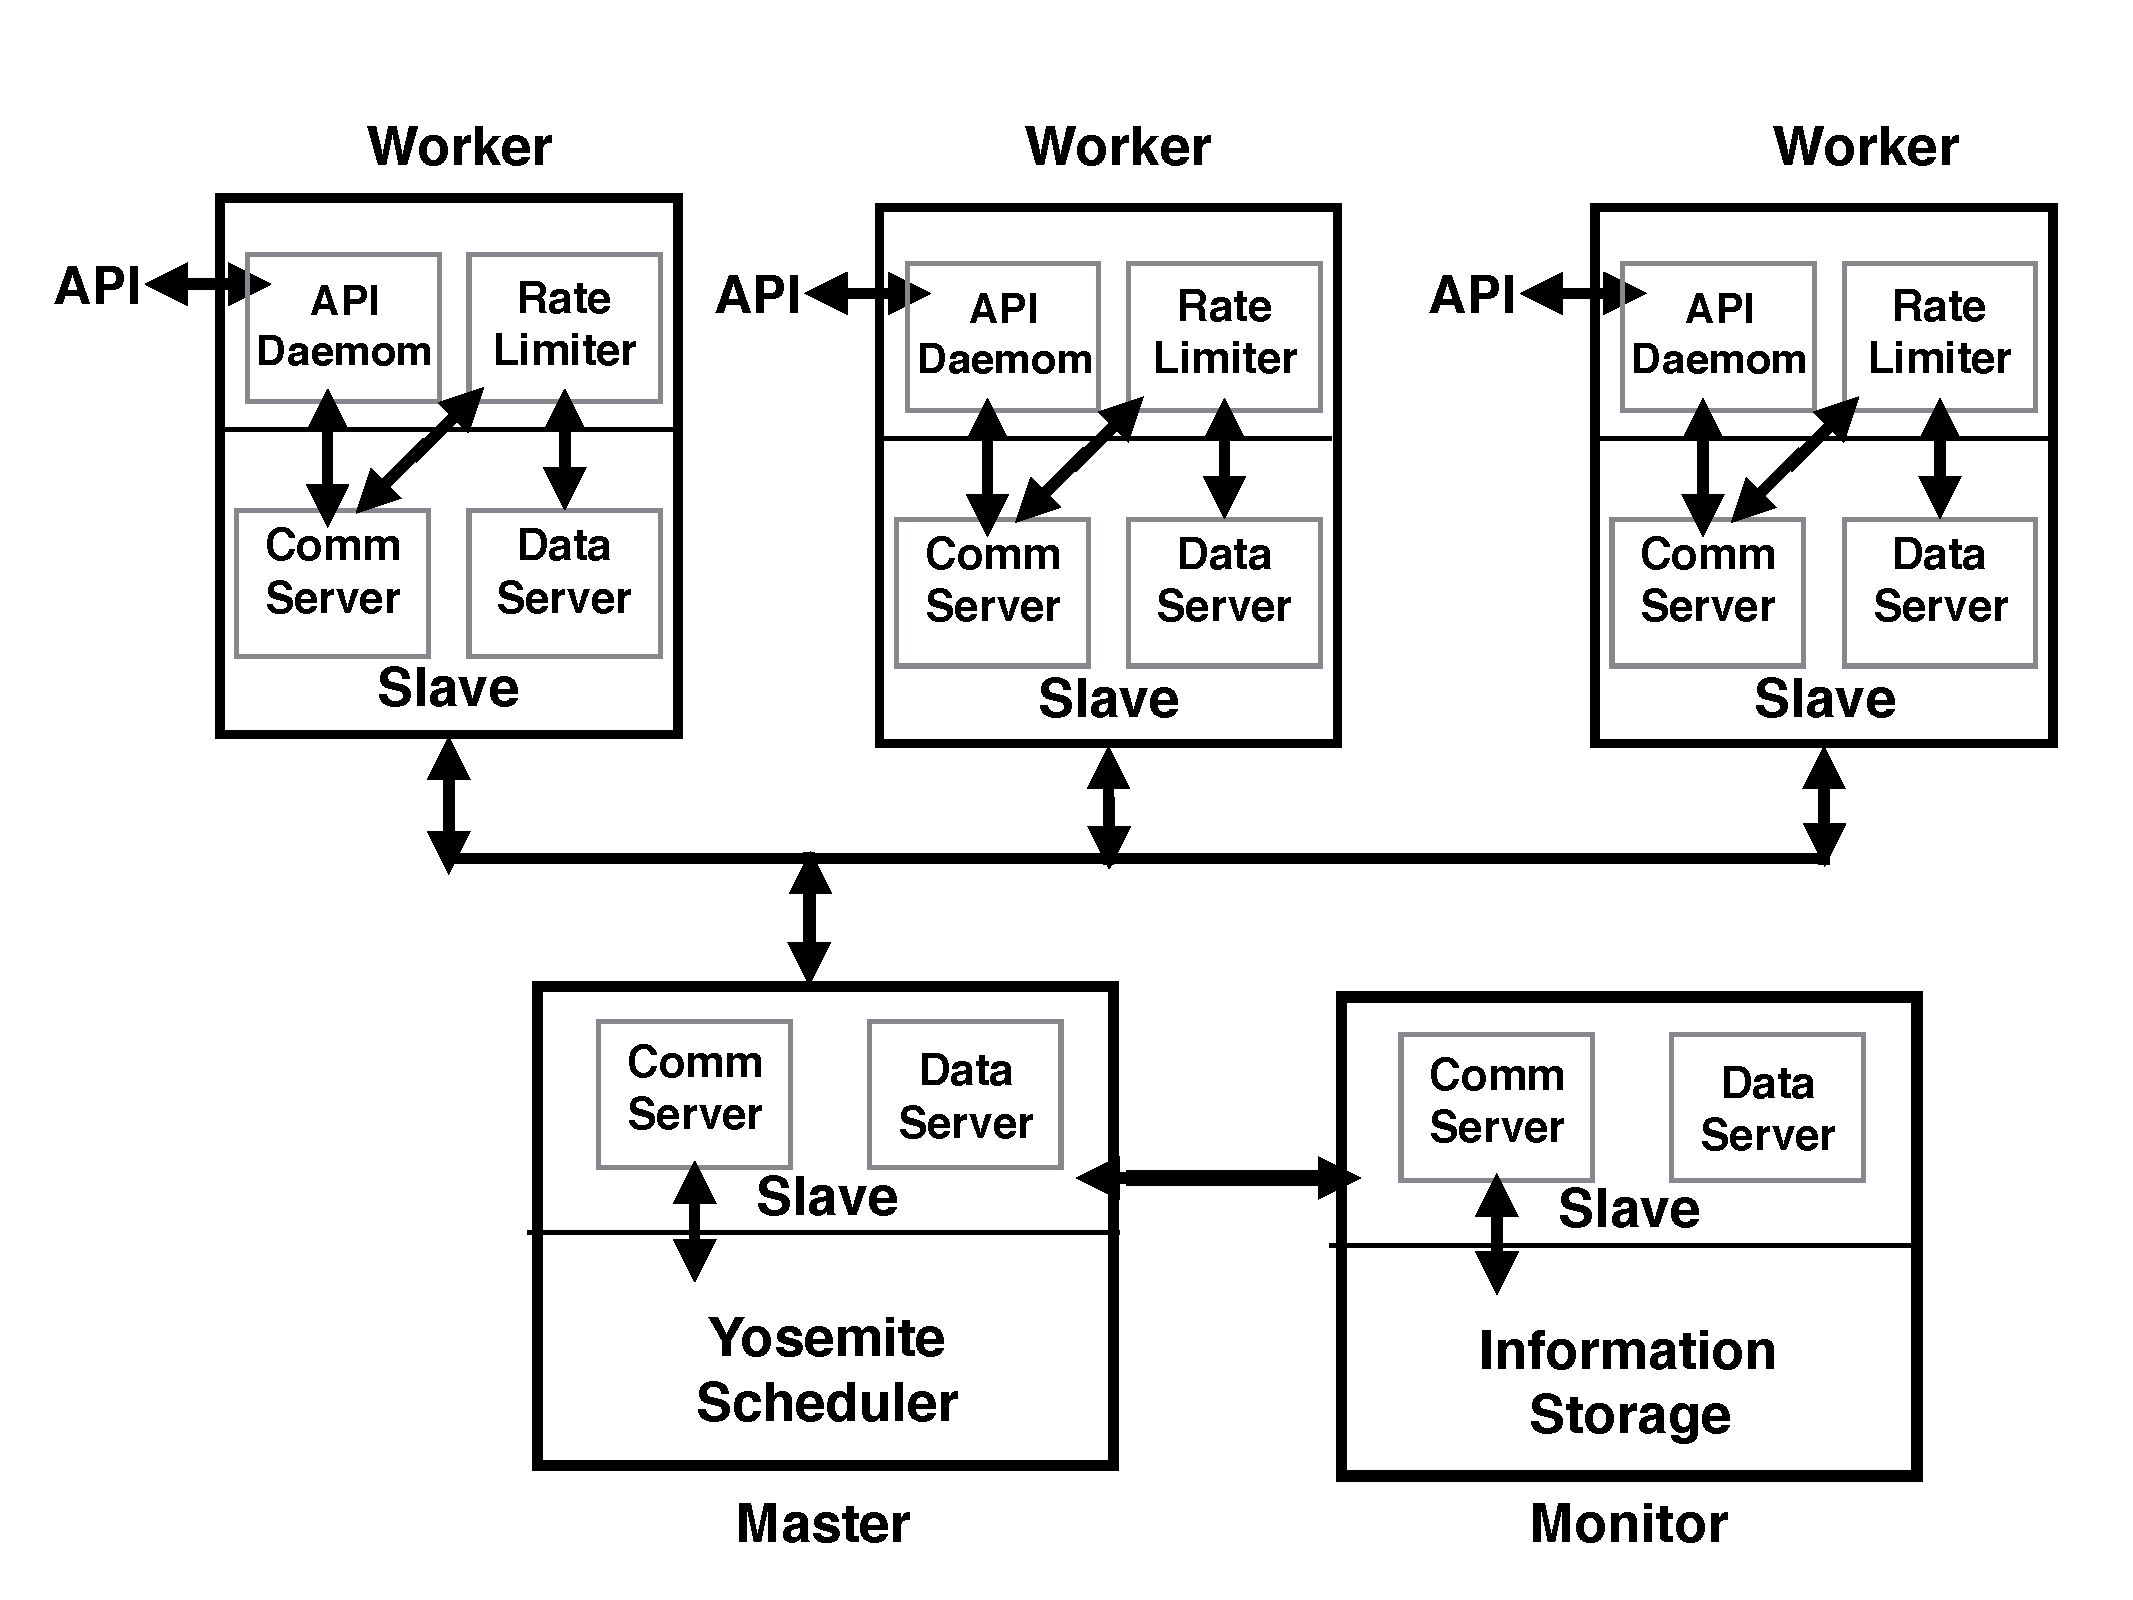
\includegraphics [width=0.8\columnwidth] {./figs/background/system.pdf}
\caption{ Architecture of the Yosemite System}
\label{System-design-fig}
\end{center}
\end{figure}

%\begin{algorithm} 
%\caption{Procedure of bandwidth allocate}
%\begin{algorithmic}[1]\label{bandwidth_allocate}
%\renewcommand{\algorithmicrequire}{\textbf{Input: }}
%\renewcommand{\algorithmicensure}{\textbf{Output:}}
%\REQUIRE Sorted coflow set $\gamma$, Remaining capacity for ports set $Rem(.)$
%\ENSURE  bandwidth of each coflow, Remaing capacity for ports set $Rem(.)$
%\FOR{k $\in \gamma$ }
% \STATE Compute Load $g^{(k)}$ according to (\ref{weight_completion_gamma})
% \FOR{$f_{i,j}$$ \in k$ }
% \STATE $b_{i,j}=f_{i,j}/g^{(k)}$
%\STATE $Rem(P_i^{(in)})-=b_{i,j}$
%\STATE $Rem(P_j^{(out)})-=b_{i,j}$
% \ENDFOR
%\ENDFOR
%\end{algorithmic} 
%\end{algorithm}

\iffalse
\begin{algorithm} \label{procedure_master}
\caption{Procedure of the scheduler}
\begin{algorithmic}[1]\label{scheduler}
\renewcommand{\algorithmicrequire}{\textbf{Input: }}
\renewcommand{\algorithmicensure}{\textbf{Output:}}
\REQUIRE Ordered coflow set $\gamma$, Remaining capacity for ingress: Rem($P^{in}_i$), Remaining capacity for egress: Rem($P^{out}_j$),
where $1 \leqslant i\leqslant m$,$1 \leqslant j \leqslant m$
\ENSURE  bandwidth of each flow 
 \FOR{F $\in \gamma$ } 
\STATE rate = $\min (\min \limits_{i}Rem(P^{in}_i),\min \limits_{j} Rem(P^{out}_i) )$,$\forall$ F goes through port i and port j, $1 \leqslant i\leqslant m$,$1 \leqslant j \leqslant m$
\STATE f.rate = rate, $\forall f \in F$ and f does not finish
\STATE $Rem(P^{in}_i)$-=rate, $1 \leqslant i\leqslant m$
\STATE $Rem(P^{out}_i) ))$-=rate, $1 \leqslant j \leqslant m$
\ENDFOR
\STATE Distribute unused bandwidth to F $\in \gamma$ 
\STATE Send result to corresponding Slave
\end{algorithmic} 
\end{algorithm}
\fi

Fig. \ref{System-design-fig} shows the architecture of Yosemite.
The system consists of three types of nodes, i.e., master, worker and monitor. 
The master node is the brain of the system. It collects coflow information from workers, 
performs coflow prioritization and bandwidth computation according to Algorithm \ref{online-algorithm},
and sends bandwidth allocation results back to workers. 
Each worker node is composed of a daemon that interacts with applications by a set of APIs, 
a rate limiter responsible for throttling flow rates, 
a comm server that communicates with the master node, 
and a data server that is responsible for sending out data traffic.
The monitor node backups the coflow scheduling state of the master node in real time, 
so that if the master node crashes, the monitor can restart the master and restore its state.

 
%Algorithm \ref{scheduler} is called when a flow starts or ends.
%Line2 computes gets the minimal value of port capacity that coflow F goes through and uses the rate as the coflow rate.
%Line4 $\sim$ Line5 updates the capacity for ingress and egress.
%Line 7 allocates the remaining bandwidth to coflows to avoid bandwidth wastes.
%At last, send the result back to senders.
%calls Algorithm \ref{bandwidth_allocate} to compute the bandwidth of coflows.
%Algorithm \ref{bandwidth_allocate} has two key steps. 
%Firstly, it computes the bottleneck time of each coflow.
%The computation method is: 
%\begin{eqnarray} \label{weight_completion_gamma}
%g^{(k)}=\max(\max \limits_i \frac{ \sum_{j=1}^mf_{i,j}^{(k)}}{Rem(P_i^{(in)})},\max \limits_j \frac{ \sum_{i=1}^mf_{i,j}^{(k)}}{Rem(P_j^{(out)})})
%\end{eqnarray}
%Where Rem(.) denotes the remaining bandwidth of an ingress or egress port estimated by the scheduler.
%(\ref{weight_completion_gamma}) computes out transfer time of the slowest flows that belongs to coflow $F^{(k)}$.
%After this, on the basis of bottleneck time, it computes bandwidth $b_{i,j}$ for each flow that transfers from port i to port j 
%Then master updates port available bandwidth as Line5$\sim$Line6 shown.  
%After the process of Algorithm.\ref{bandwidth_allocate}, scheduler calculates out bandwidth for each flow.

%In particular, communication between components is important for a correct distributed, concurrent, fault-tolerant and scalable application.
%As messages transferring between components needs timely responds, keeping responsive in the face of failure, staying responsive under varying workload. 
%In Yosemite, Comm Server is responsible for this. 
%Comm Server extends Akka \cite{Akka}. 
%Using the library provided by Akka, Comm Server can provide stable communication for Yosemite components. 

 

%\subsection{API}
%Yosemite provides API like DOT \cite{tolia2006architecture} and Varys \cite{chowdhury2014efficient} to abstract the underlying scheduling and communication mechanisms. 
%User jobs do not require any modifications, but should create Yosemite client to interact with the master. 
%The client of Yosemite provides 4 key API just as Table. \ref{tab:API} shown.
%
%\begin{table}[!htb]
%          \centering
%          \footnotesize
%          \caption{Yosemite API} \label{tab:API}
%          \begin{tabulary}{\textwidth}{ccccr}
%              \toprule
%              Name  & \multicolumn{1}{c}{parameters} & Return & Description \\
%              \midrule
%              \multicolumn{1}{r}{RegisterCoflow} & coflowdesc,weight    & coflowId     & Regisger a coflow \\
%              \multicolumn{1}{r}{Send} & coflowId,size,dst    & bool     & Send size data to dst \\
%              \multicolumn{1}{r}{Receive} & coflowId    & bool     & Receive a flow \\
%              \multicolumn{1}{r}{ReleaseCoflow} & coflowId,   & bool     & Release coflow \\
%              \bottomrule
%          \end{tabulary}
%      \end{table}
%      
%     
%Register takes coflow description and weight of the coflow as parameters.
%After sending the register information to master, coflow id will be returned to worker node.
%Send tasks coflowId and IP address of destination node as parameters.
%This method sends a flow that belongs to coflowId.
% Receive tasks coflowId as the parameter.
% This method is used to receive data belongs to the corresponding coflow.
% If return true, denoting worker receivers data successfully. 
% Otherwise it will return false.
%ReleaseCoflow takes coflowId as the parameter and it is used to release the coflow when all flows belong to the coflow finish transferring.




\section{evaluation} \label{evaluation}

In this section, we test the performance of Yosemite in both simulation and testbed.
We evaluate Yosemite at our openstack \cite{openstack} platform, which
 can run 80 virtual machines (2 Cores, 4GB Memory) simultaneously. 
For larger scale experiments, we use trace-driven simulation. 
Main results of our evaluation are as follows:

%\begin{figure}[b]
%\begin{center}
%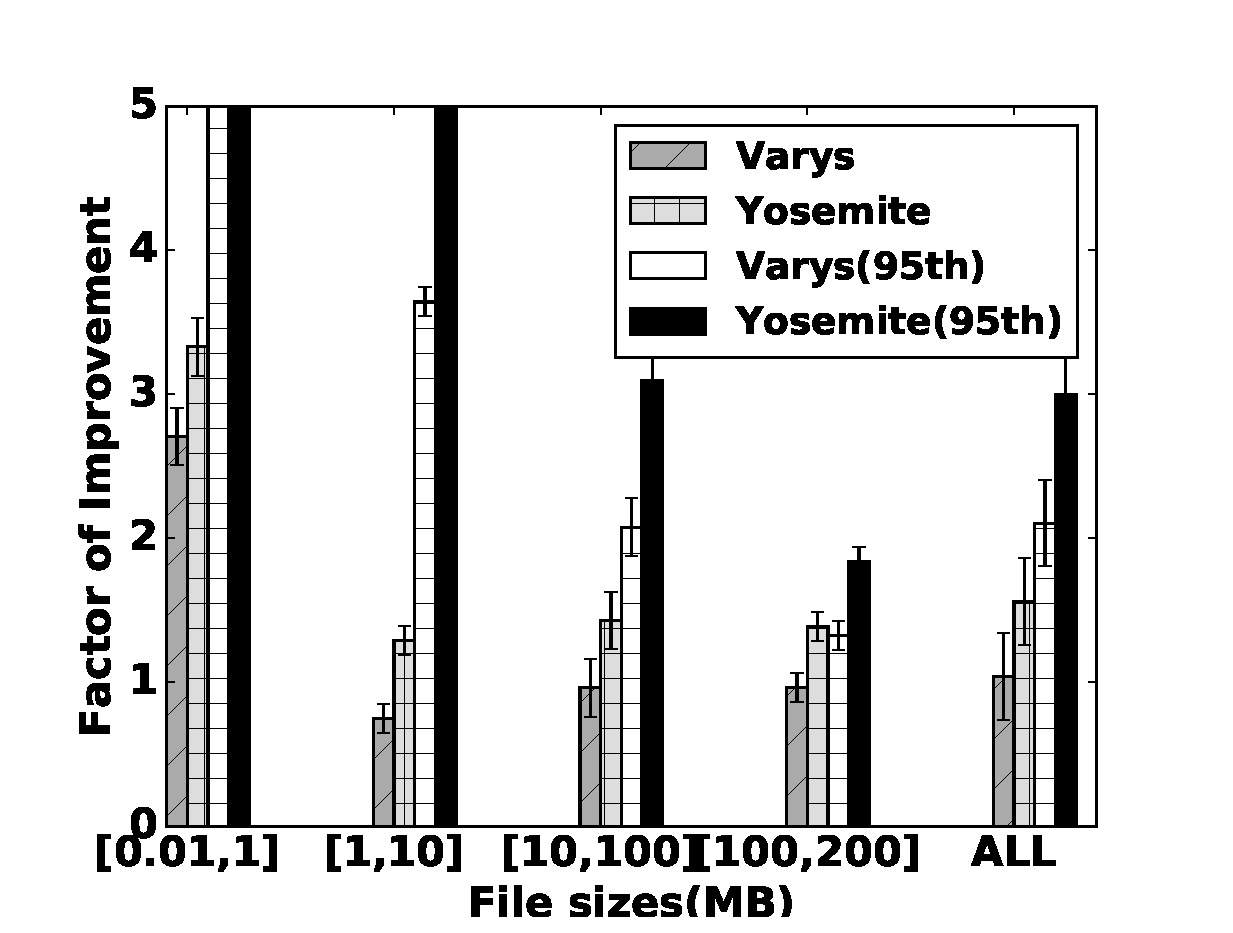
\includegraphics [width=1.0\columnwidth] {./figs/fake/fake2.eps}
%\caption{[Cloud] File distribute application performance}
%\label{distribute-fig}
%\end{center}
%\end{figure}





\begin{itemize}[\IEEEsetlabelwidth{Z}]
\item For the trace of facebook\cite{chowdhury2014efficient} with random weight, 
Yosemite improves about $30\%$, $40\%$, $50\%$ over Varys \cite{chowdhury2014efficient}, Aalo \cite{chowdhury2015efficient} and Barrat \cite{dogar2014decentralized} on reducing average weighted coflow completion time. For coflows with above-the-average level of emergence, 
Yosemite performs about $20\%$ ,$ 30\%$, $40\%$ better than Varys, Aalo, Barrat.
\item  For the trace of our data center, Yosemite performs about 30\% better than Varys, which is the best performing one among existing coflow scheduling algorithms on reducing emergency coflows' average completion time.
\item Comparing with the 2-approximation greedy algorithm, the non-clairvoyant online algorithm has less than $30\%$ performance loss.
\item Real testbed shows, Yosemite can improve about 25\%-30\% on reducing the emergency coflows' average completion time.
The computation time of Yosemite is short, with $\sim$23ms on average, which occupies about $0.1\%$ of the total transfer time.
\end{itemize}



\subsection{methlogy}

\textbf{Experiment settings and Metrics}
In our simulations, we use two real world traffic trace. 
The first one is from our data center, in which 100 applications running simultaneously among about 720 servers deployed in 60 racks.
We have 5 level of emergence for applications' coflows: Significant, Important, Normal, Unimportant, Lax.
In our algorithm, urgent coflows have higher weight and less important ones have lower weight.
In our experiments, default corresponding weight value  for  Significant, Important, Normal, Unimportant, Lax are 5, 4, 3, 2, 1.
Traffic of Facebook that was collected from a 3000-machine cluster with 150 racks \cite{chowdhury2014efficient}. 
As the original trace does not contain information of weight settings, we randomly select weight within 1, 2 ,3, 4, 5 for coflows to present their emergence.

 In our experiment,  we use two metrics to estimate different methods.
The first metrics is average coflow completion time (CCT) for different weight coflows. 
Coflows are categorized to be five types in terms of importance: Significant, Important, Normal, Unimportant, Lax.
In some cases, TCP is chosen as the baseline and we define the factor of improvement=$\frac{baseline\; avg \;CCT}{current\;avg \;CCT}$.
The second metrics is average weighted coflow completion time (WCCT).
Coflows are categorized to be four types in terms of their length (the size of the largest flow in bytes for a coflow) and width (the number of parallel flows in a coflow): Narrow\&Short(N-S), Narrow\&Long(N-L), Wide\&Short(W-S), and Wide\&Long(W-L), where a coflow is considered to be short if its length is less than 100 MB, and narrow if it involves at most 20 flows.
In some cases, TCP is chosen as the baseline and we define factor of improvement for WCCT=$\frac{baseline\; avg \;WCCT}{current\;avg \;WCCT}$.



\begin{figure*}[!t]
\centering
\subfigure[Average WCCT ] {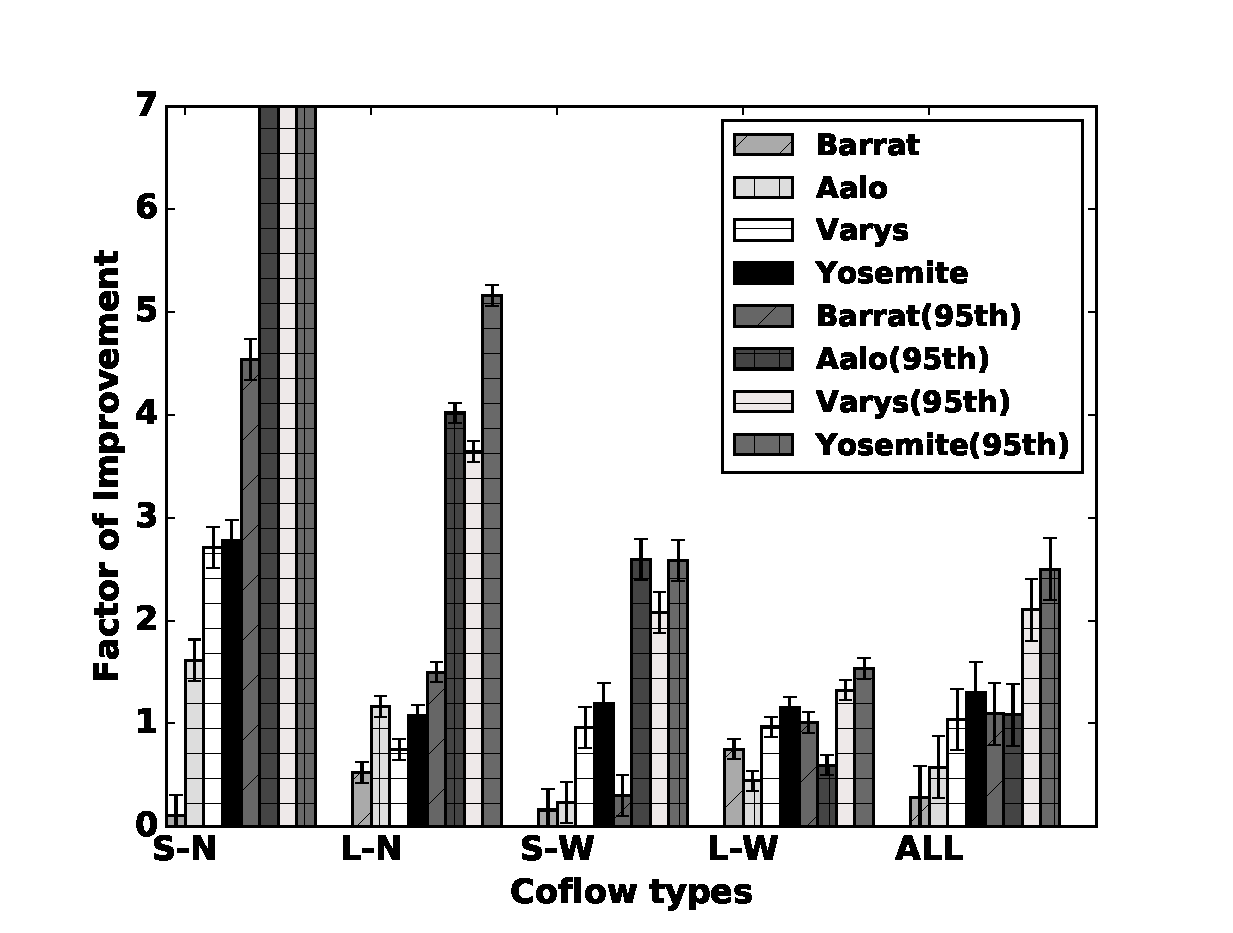
\includegraphics[width=1.6  in]{./figs/evaluation/ex2/weight_real_type.eps}}
\hspace{0.1in}
\subfigure[WCCT distribution ] {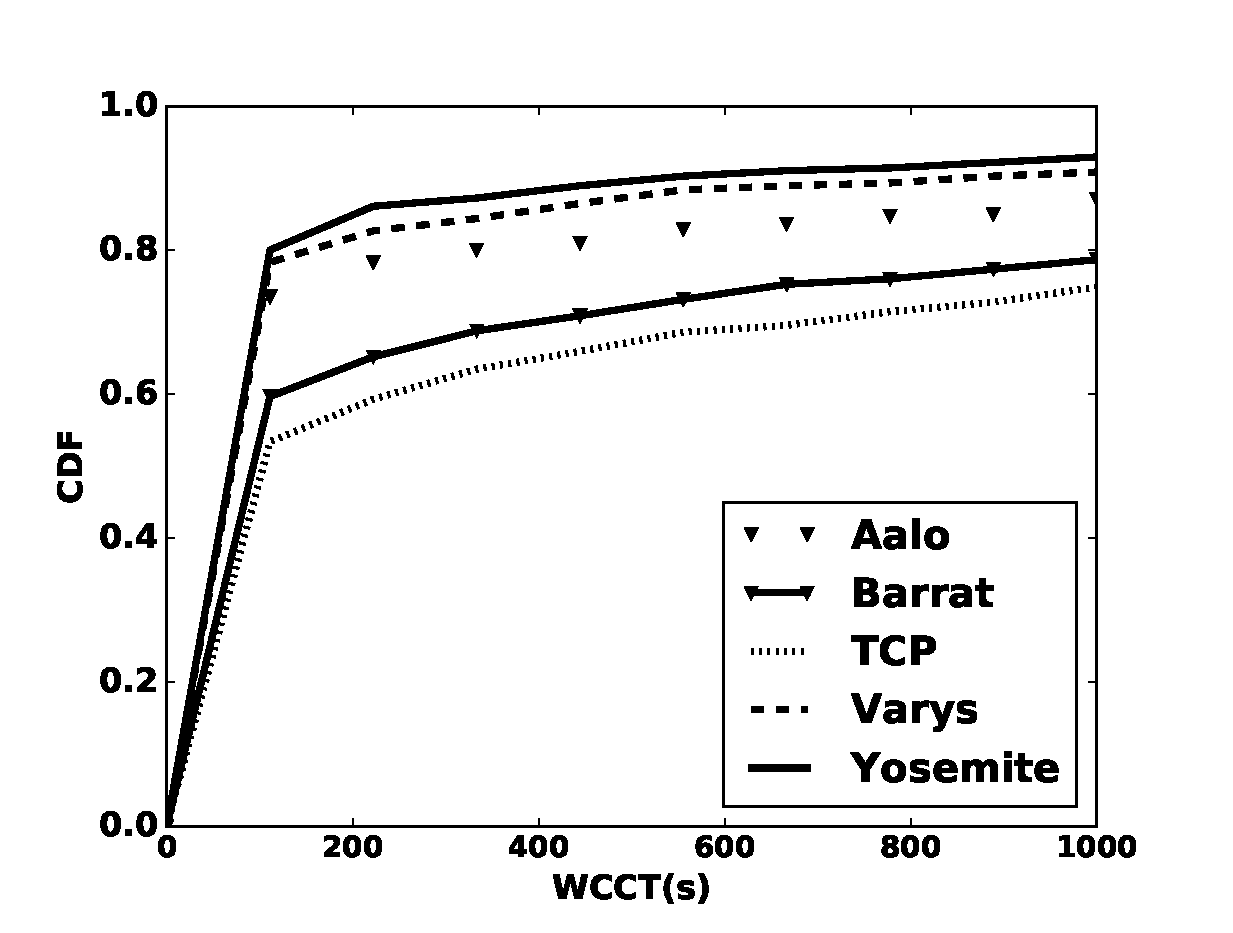
\includegraphics[width=1.6  in]{./figs/evaluation/ex2/weight_CDF_compare.eps}}
\hspace{0.1in}
\subfigure[Average CCT ] {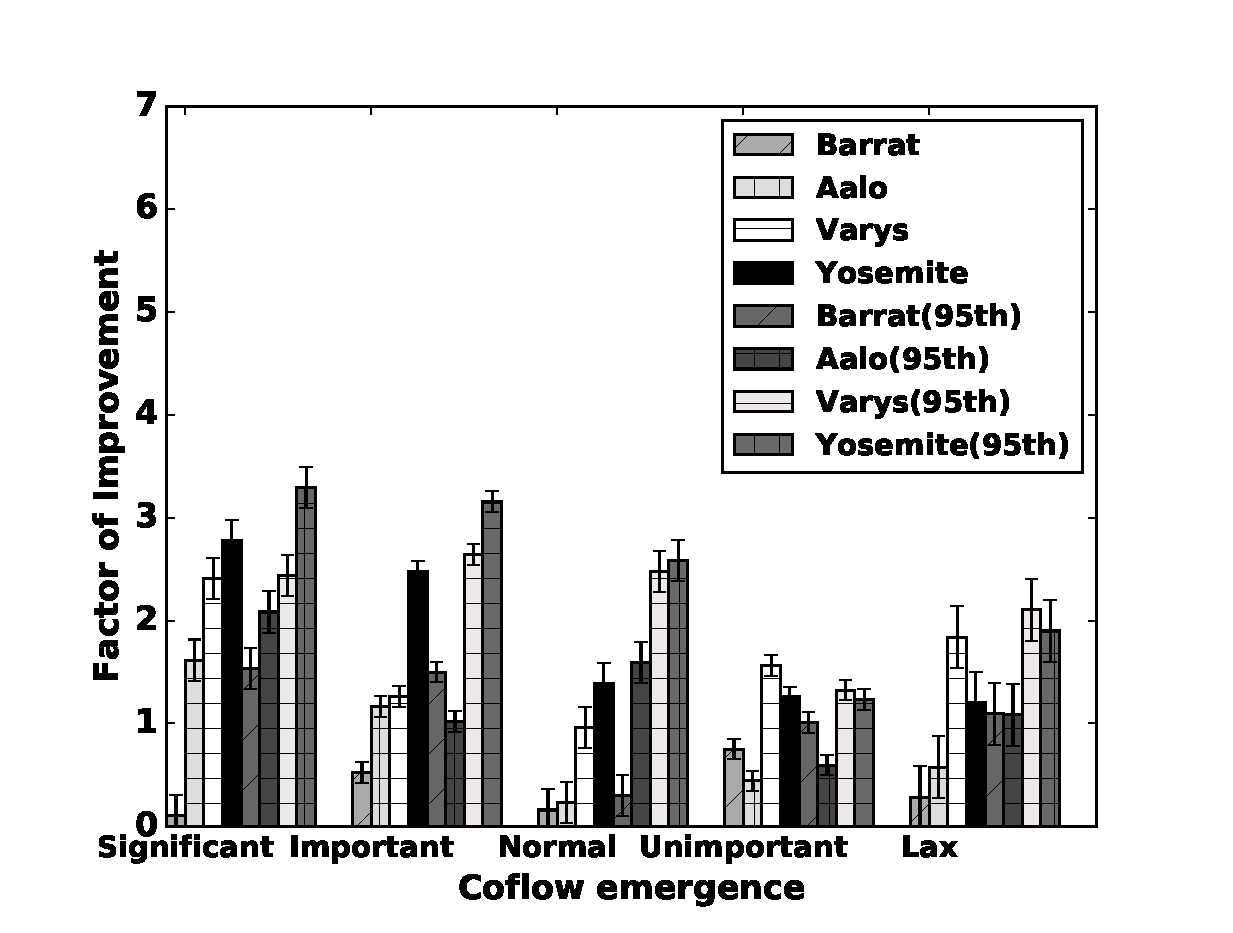
\includegraphics[width=1.6  in]{./figs/evaluation/ex2/nfake1.eps}}
\hspace{0.1in}
\subfigure[CCT distribution  ] {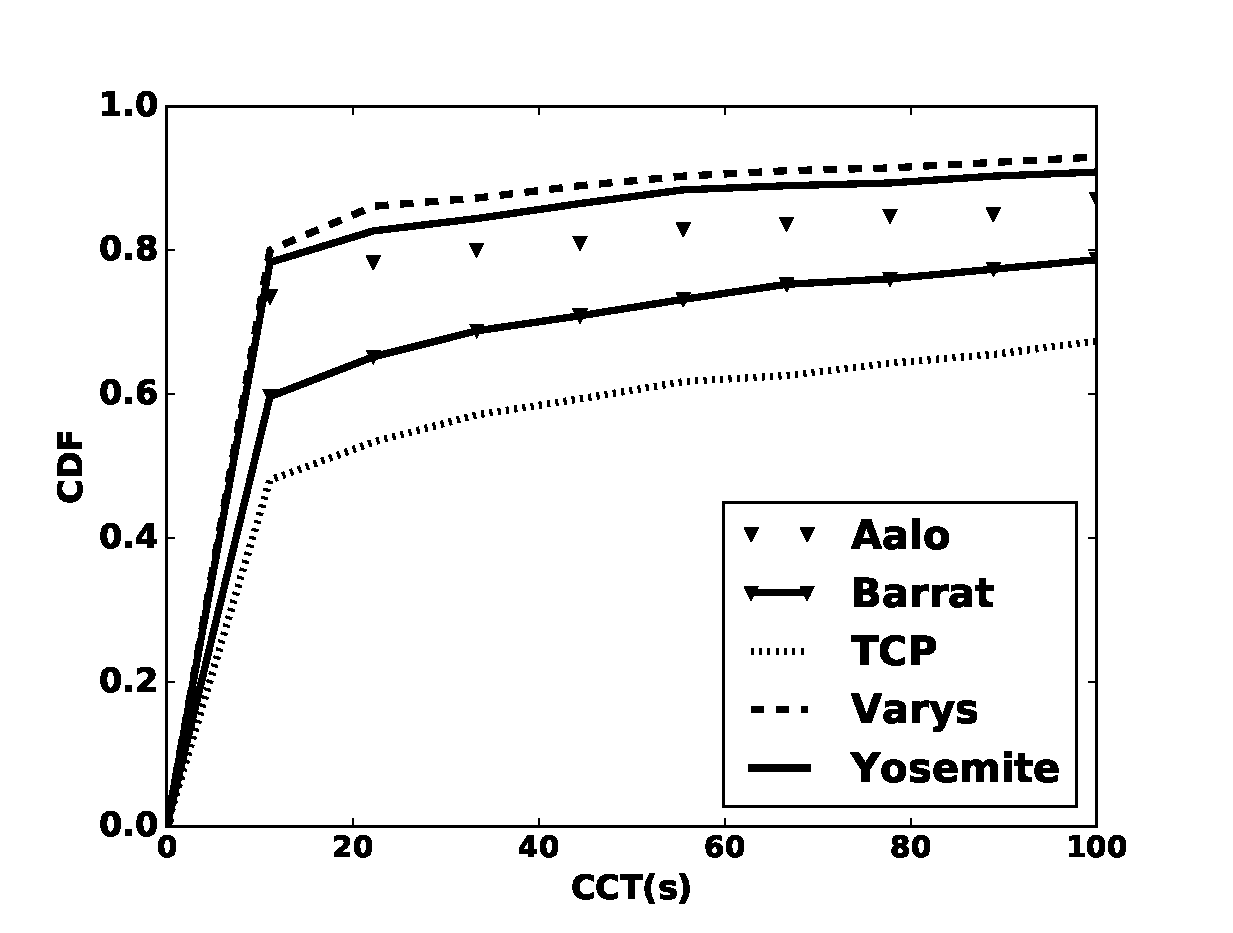
\includegraphics[width=1.6  in]{./figs/evaluation/ex2/CDF_compare.eps}}
\vspace{-0.1 in}
\caption{[Simulation] Average WCCT and average CCT comparison for facebook trace, TCP is selected as the baseline.}
\label{evaluation_facebook_fig}
\vspace{-0.1 in}
\end{figure*}


\begin{figure*}[!t]
\centering
\subfigure[Average WCCT] {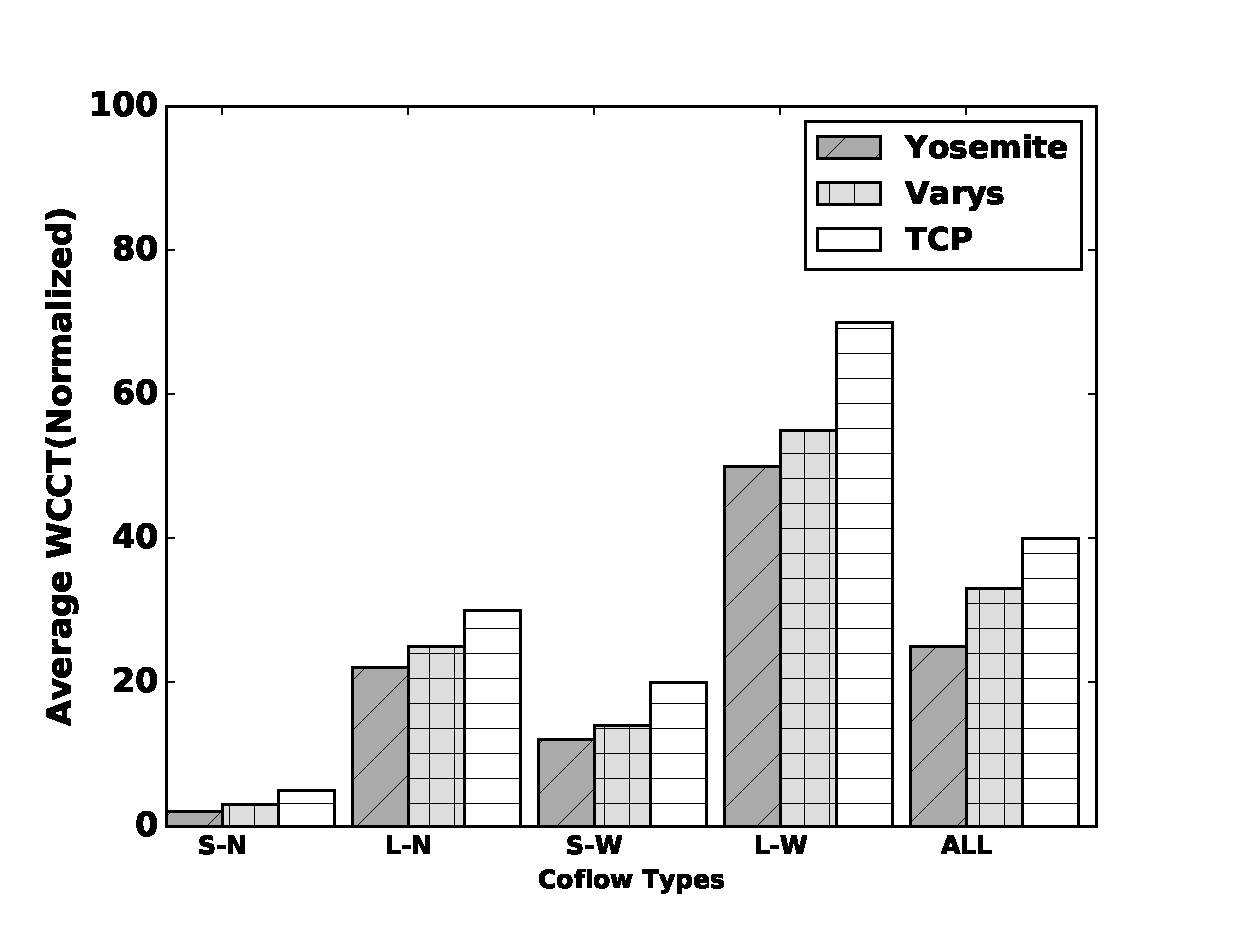
\includegraphics[width=1.65 in]{./figs/evaluation/ex1/evaluation_motivation1.eps}}
\hspace{0.1in}
\subfigure[Average CCT] {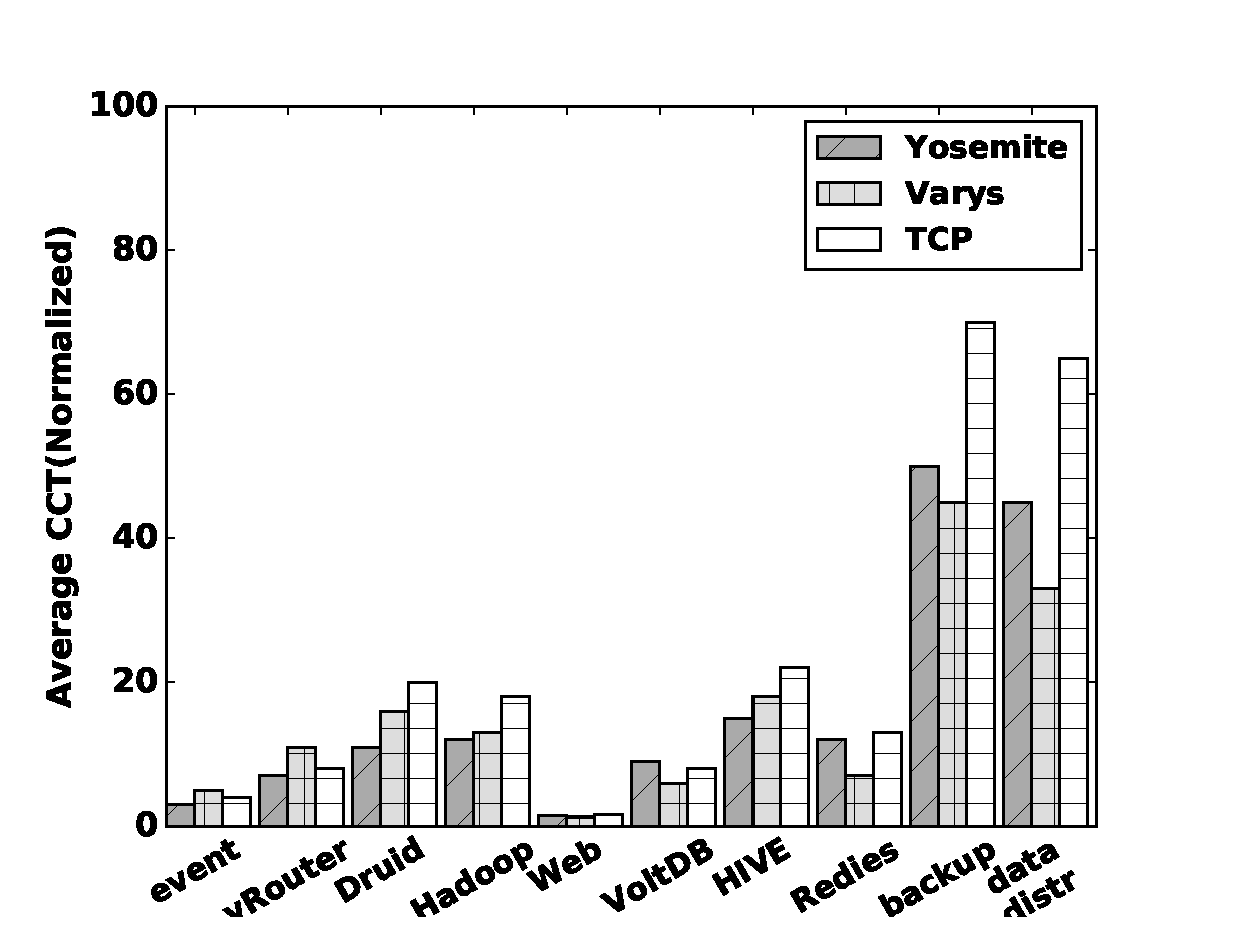
\includegraphics[width=1.65 in]{./figs/evaluation/ex1/evaluation_motivation2.eps}}
\vspace{-0.1 in}
\subfigure[Hadoop WCCT] {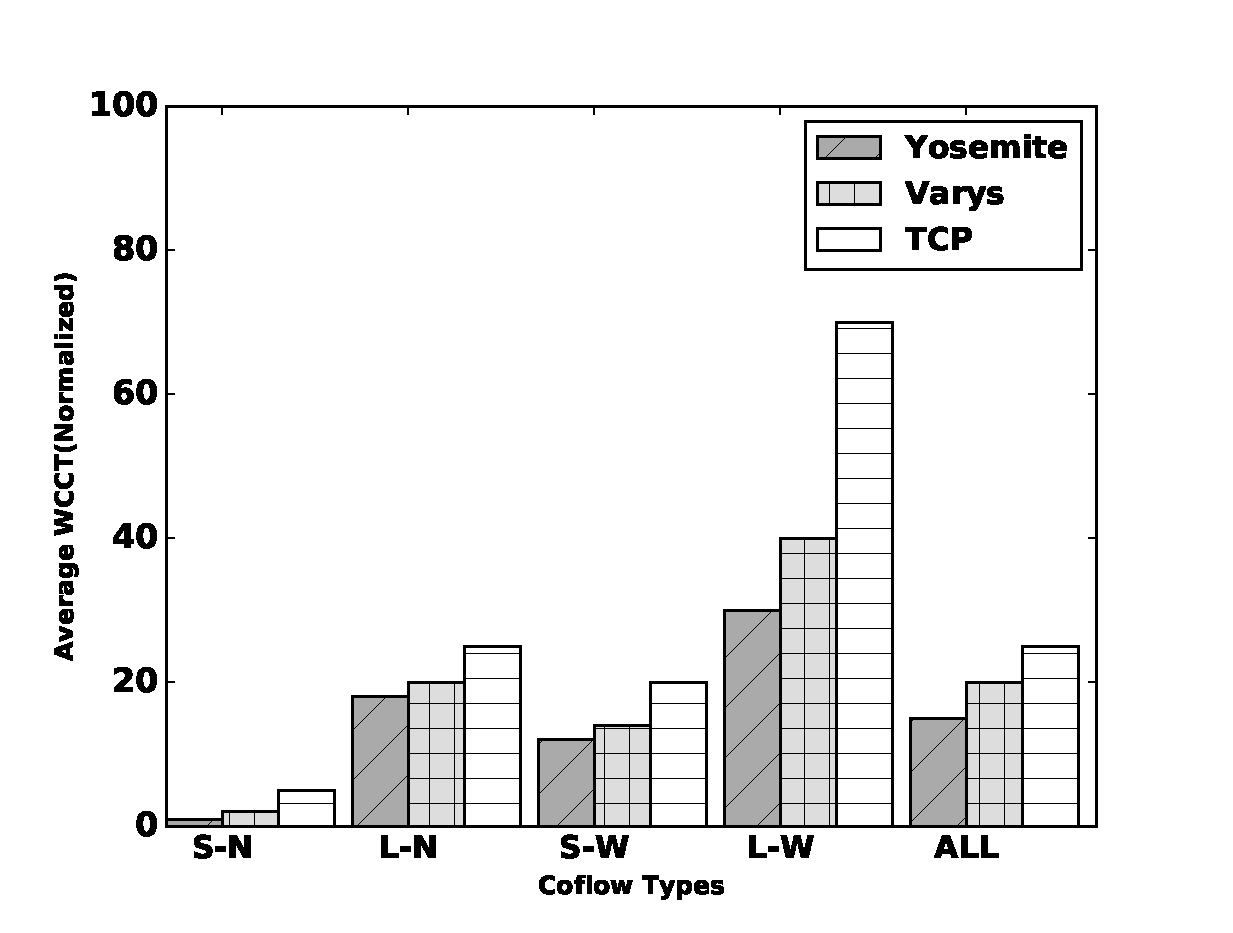
\includegraphics[width=1.65 in]{./figs/evaluation/ex1/evaluation_motivation3.eps}}
\hspace{0.1in}
\subfigure[Hadoop CCT] {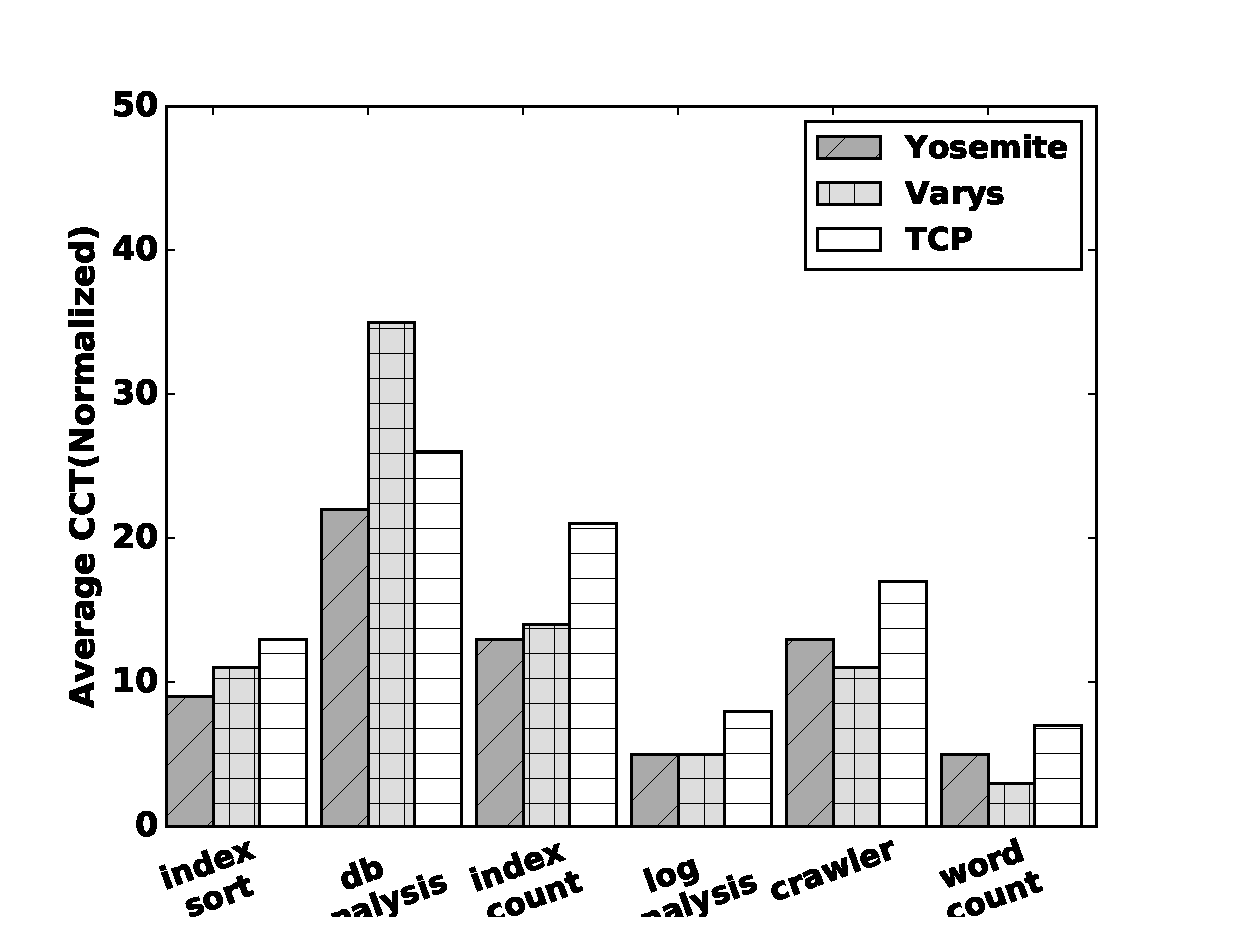
\includegraphics[width=1.65 in]{./figs/evaluation/ex1/evaluation_motivation4.eps}}
\hspace{0.1in}
\caption{[Simulation] Average CCT (Normalized)  and Average WCCT for all applications and Hadoop. Varys ignores the importance of applications ,while Yosemite considers both importance of applications and network condition. }
\label{evaluation_motivation_fig}
\vspace{-0.1 in}
\end{figure*}




\begin{figure}[!t]
\centering
\subfigure[Small wd  ] {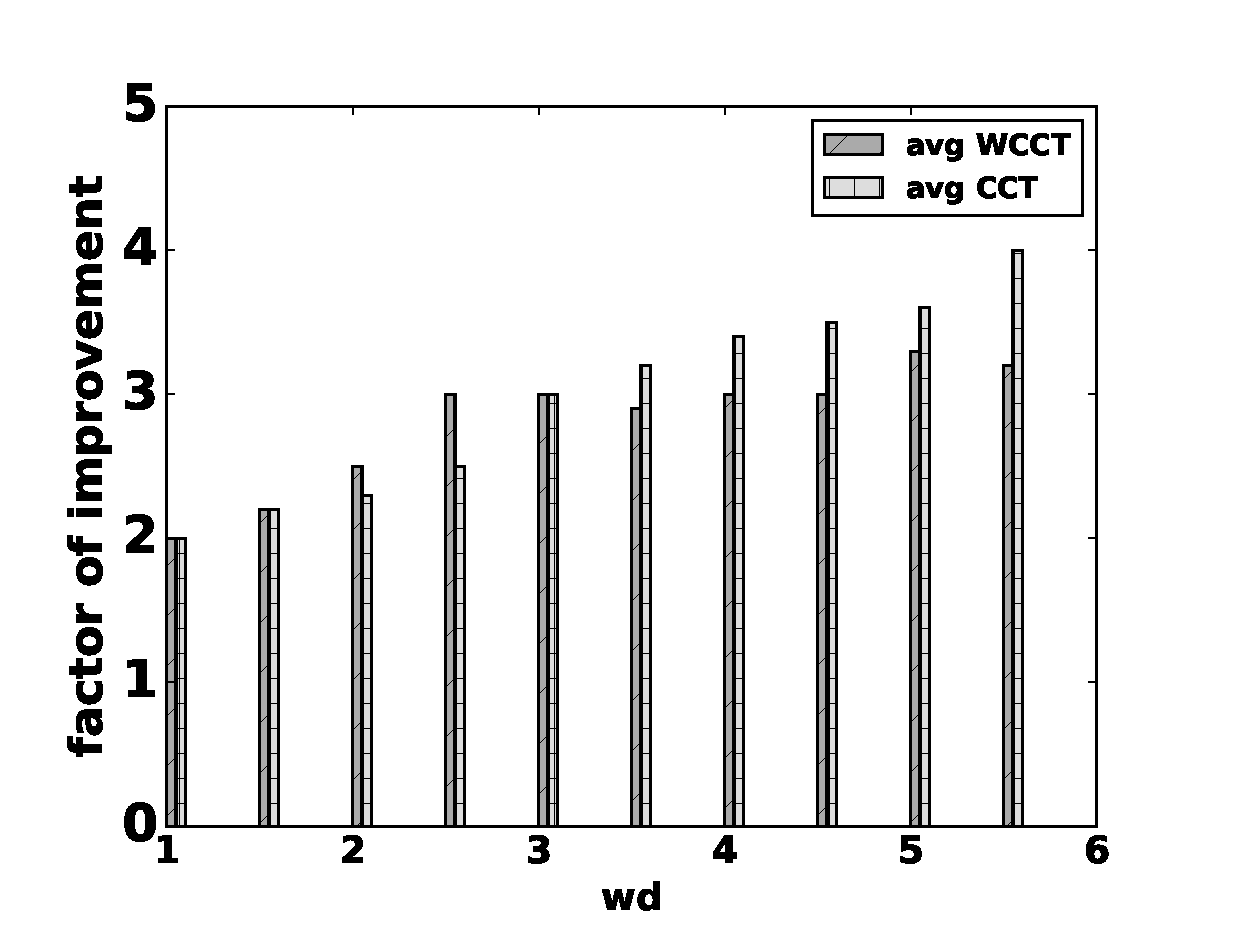
\includegraphics[width=1.6  in]{./figs/evaluation/ex3/fake7.eps}}
\hspace{0.1in}
\subfigure[Large wd ] {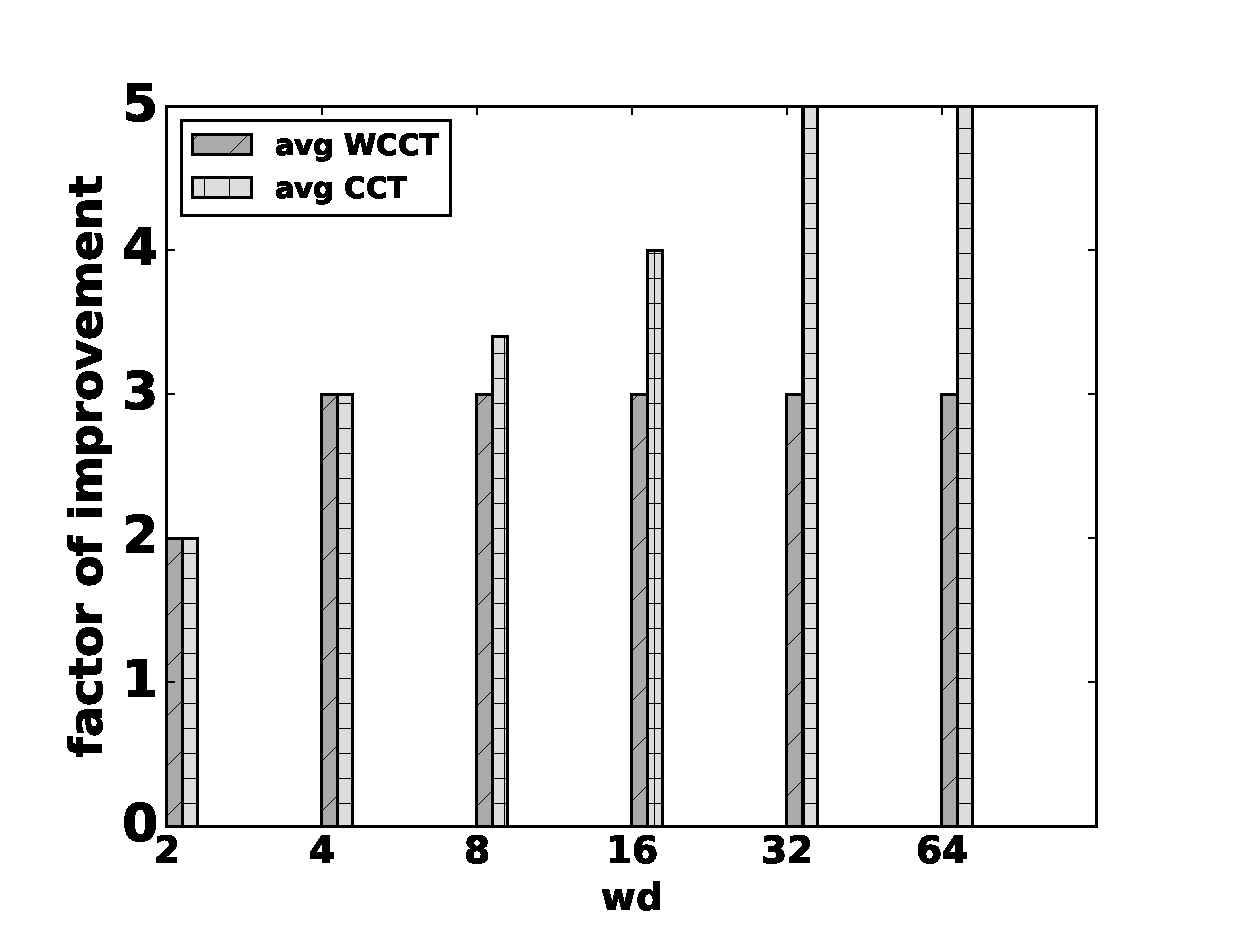
\includegraphics[width=1.6  in]{./figs/evaluation/ex3/fake8.eps}}
\hspace{0.1in}
\caption{[Simulation] Average WCCT and average CCT under different weight settings, TCP is selected as the baseline.}
\label{evaluation_weight_fig}
\vspace{-0.1 in}
\end{figure}














%\begin{figure}[b]
%\begin{center}
%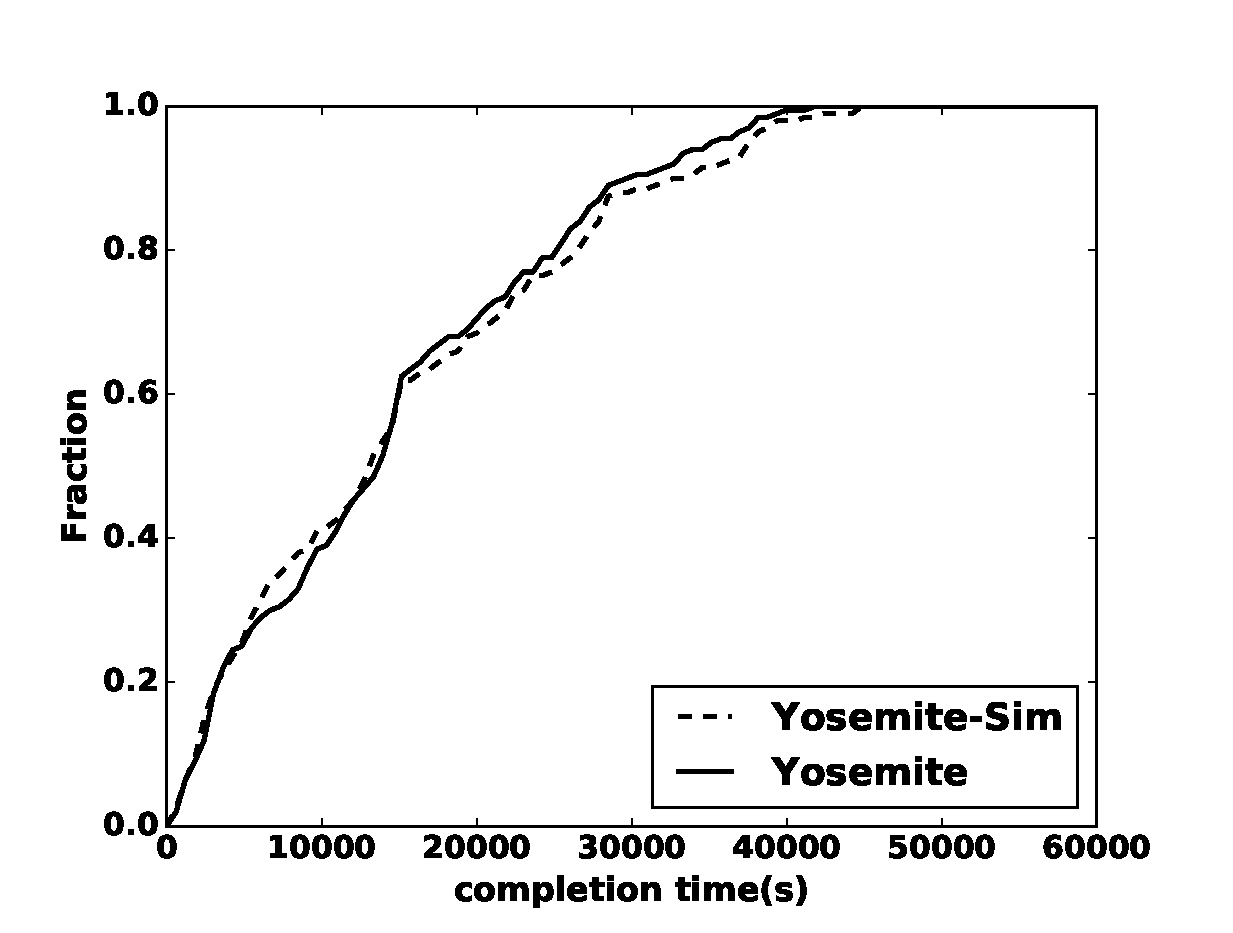
\includegraphics [width=0.8\columnwidth] {./figs/fake/fake3.eps}
%\caption{[Cloud] Performance comparison between Yosemite and Yosemite-sim under the same settings}
%\label{sim-real}
%\end{center}
%\end{figure}
%
%\begin{figure*}[!t]
%\centering
%\subfigure[Improvement of WCCT] {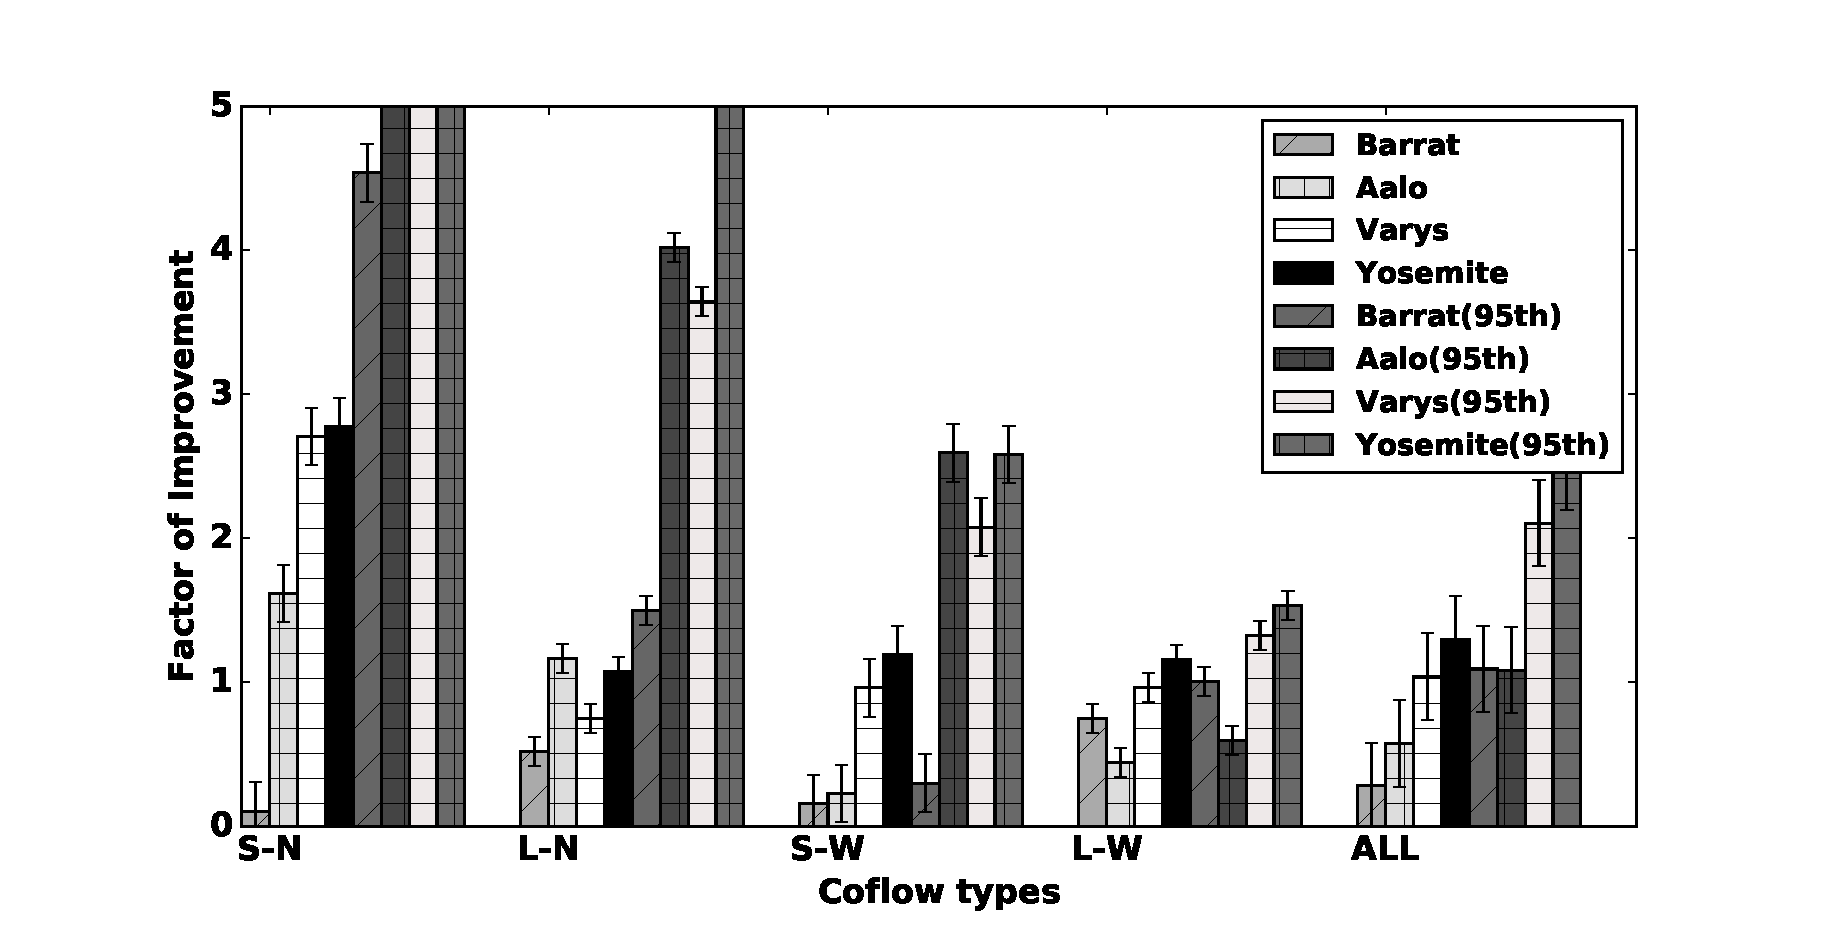
\includegraphics[width=4.9 in]{./figs/real/weight_real_type.eps}}
%\hspace{0.1in}
%\subfigure[Distribution of WCCT(s)] {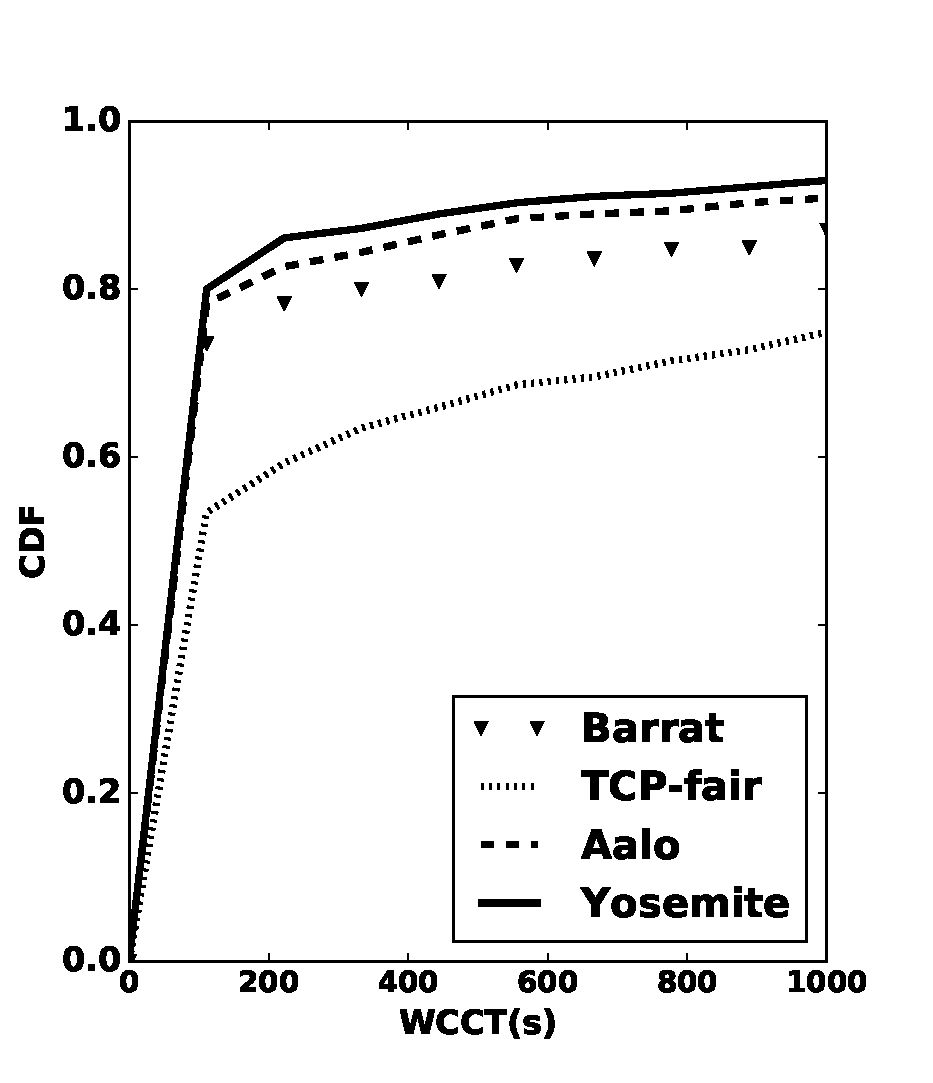
\includegraphics[width=2.05 in]{./figs/real/weight_CDF_compare.eps}}
%\caption{[Simulation] Detail of WCCT for Yosemite, Barrat, Varys,  Aalo, TCP fair-sharing under real data center traffic trace}
%\vspace{-0.1 in}
%\label{evalution_real_weight_fig}
%\vspace{-0.1 in}
%\end{figure*}
%
%
%
%\begin{figure*}[!t]
%\centering
%\subfigure[Improvement of CCT] {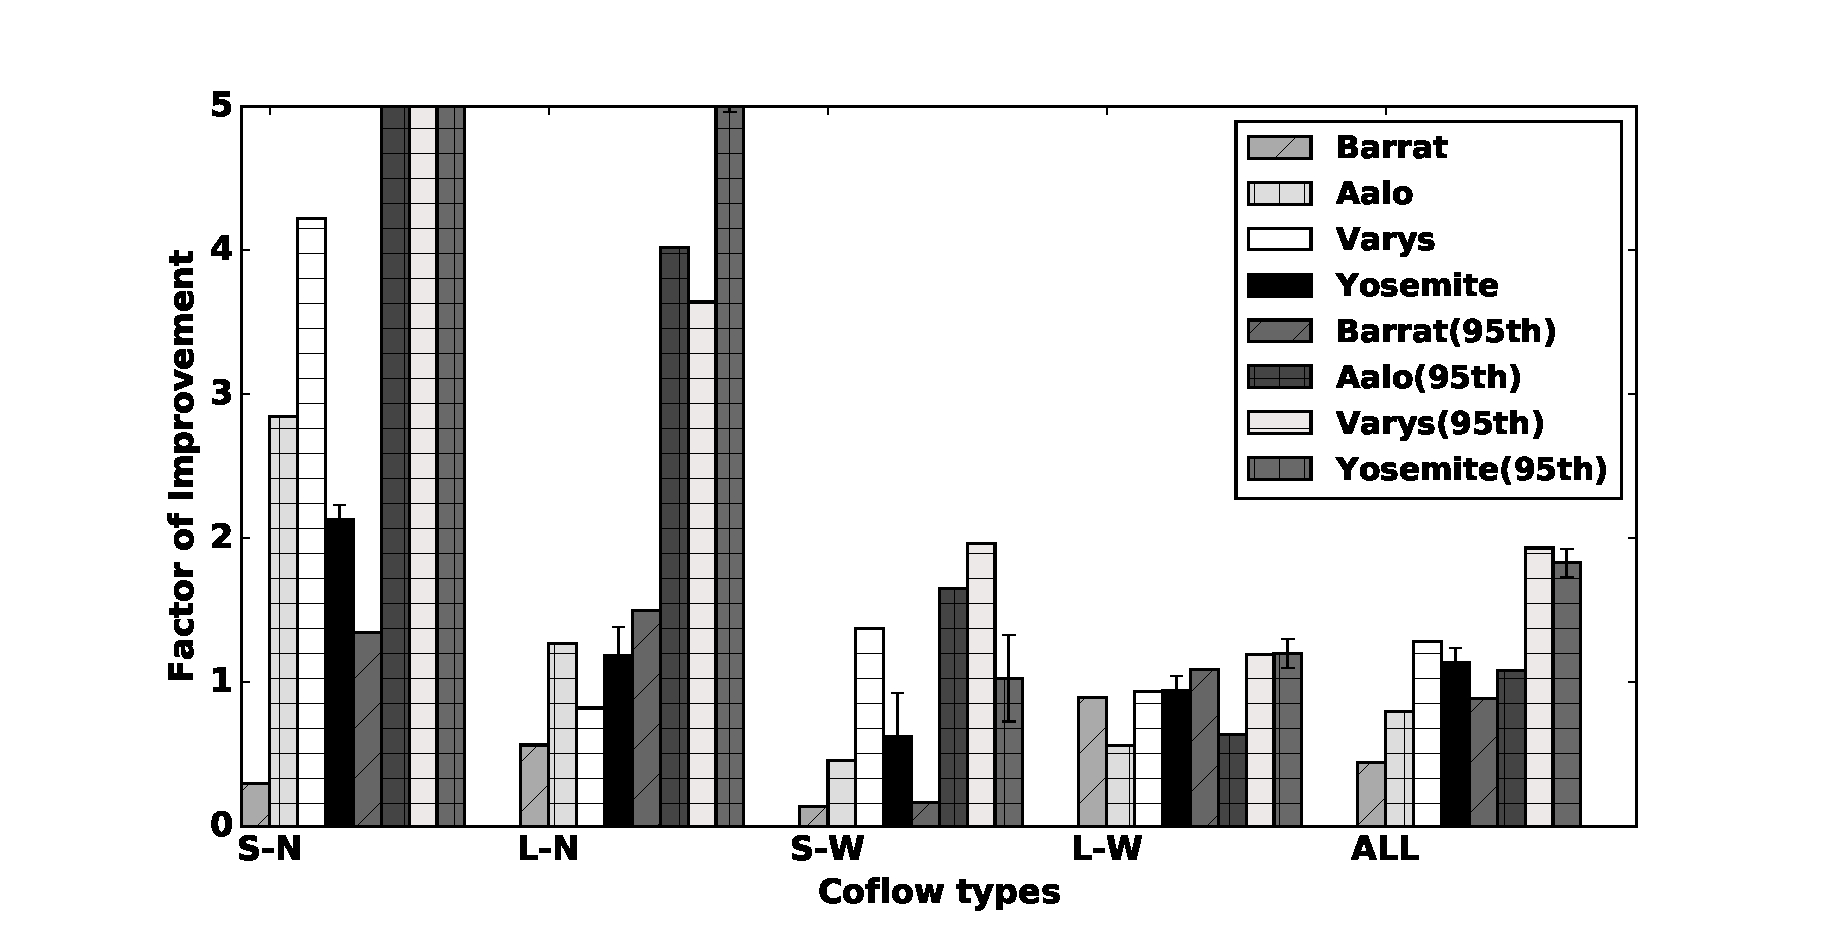
\includegraphics[width=4.9 in]{./figs/completion/real_type.eps}}
%\subfigure[Distribution of CCT(s)] {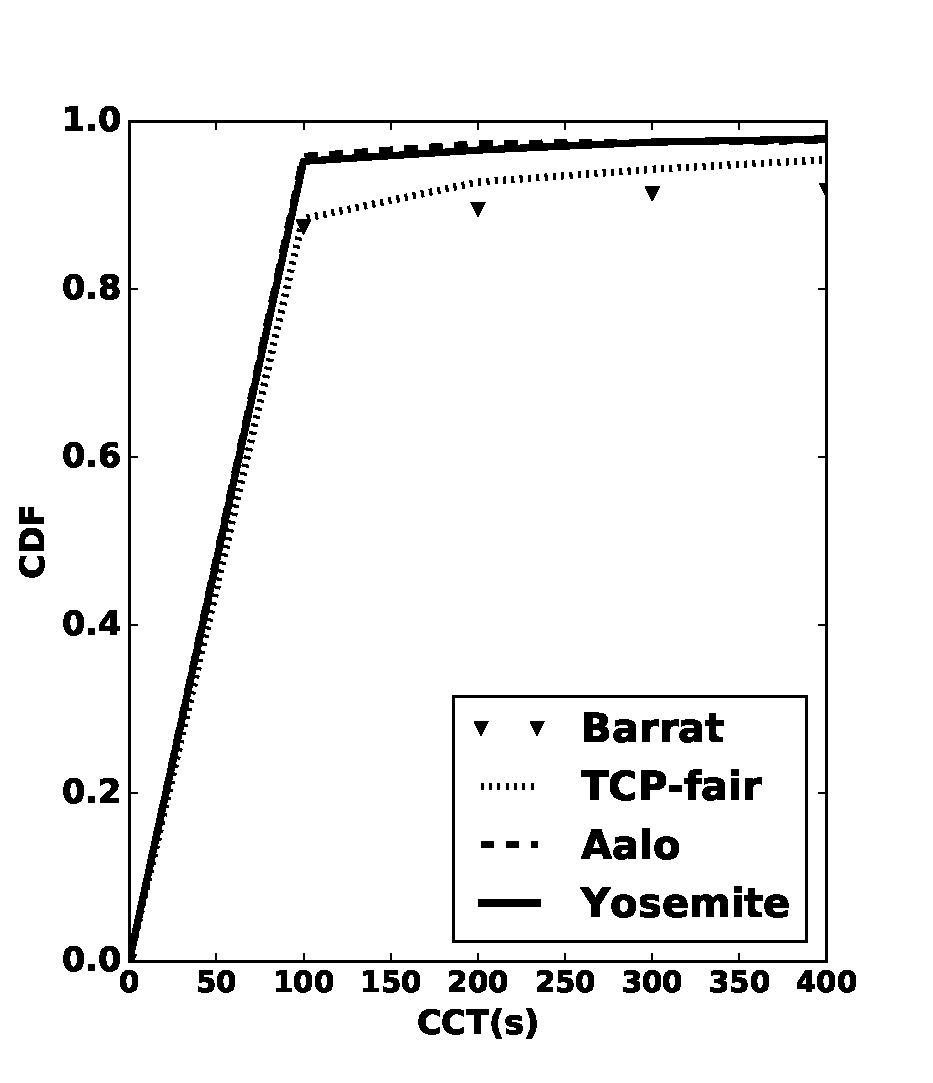
\includegraphics[width=2.1 in]{./figs/completion/CDF_compare.eps}}
%\caption{[Simulation] Detail of CCT for Yosemite, Barrat, Varys,  Aalo, TCP fair-sharing under real data center traffic trace.}
%\label{evalution_real_fig}
%\end{figure*}
%
% \begin{figure*}[!t]
%\centering
%\subfigure[Impact of coflow length] {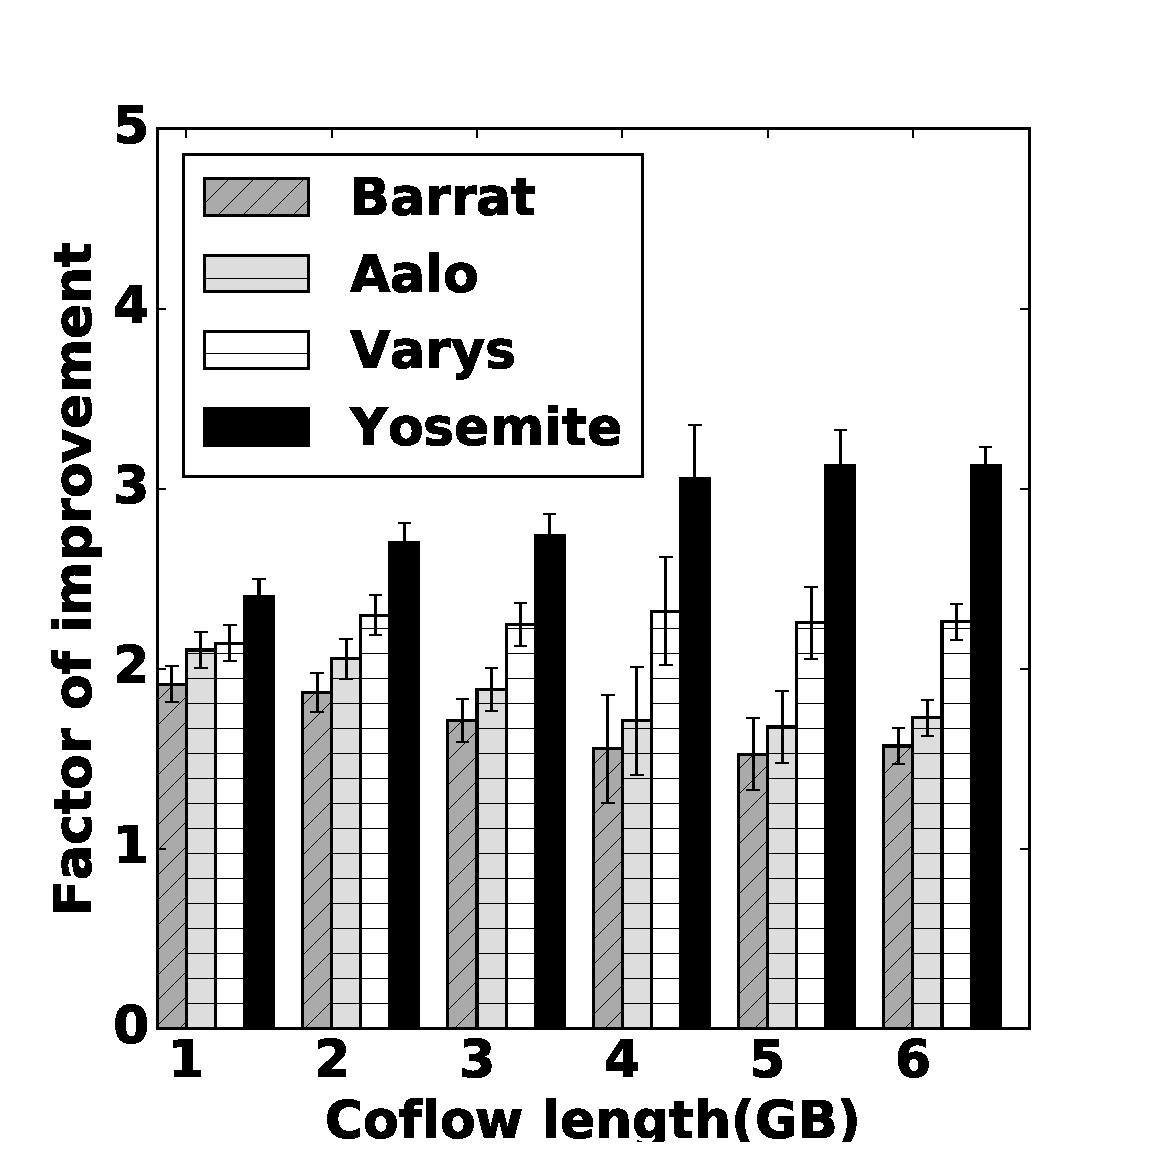
\includegraphics[width=1.65 in]{./figs/different/fraclength.eps}}
%\hspace{0.1in}
%\subfigure[Impact of coflow width] {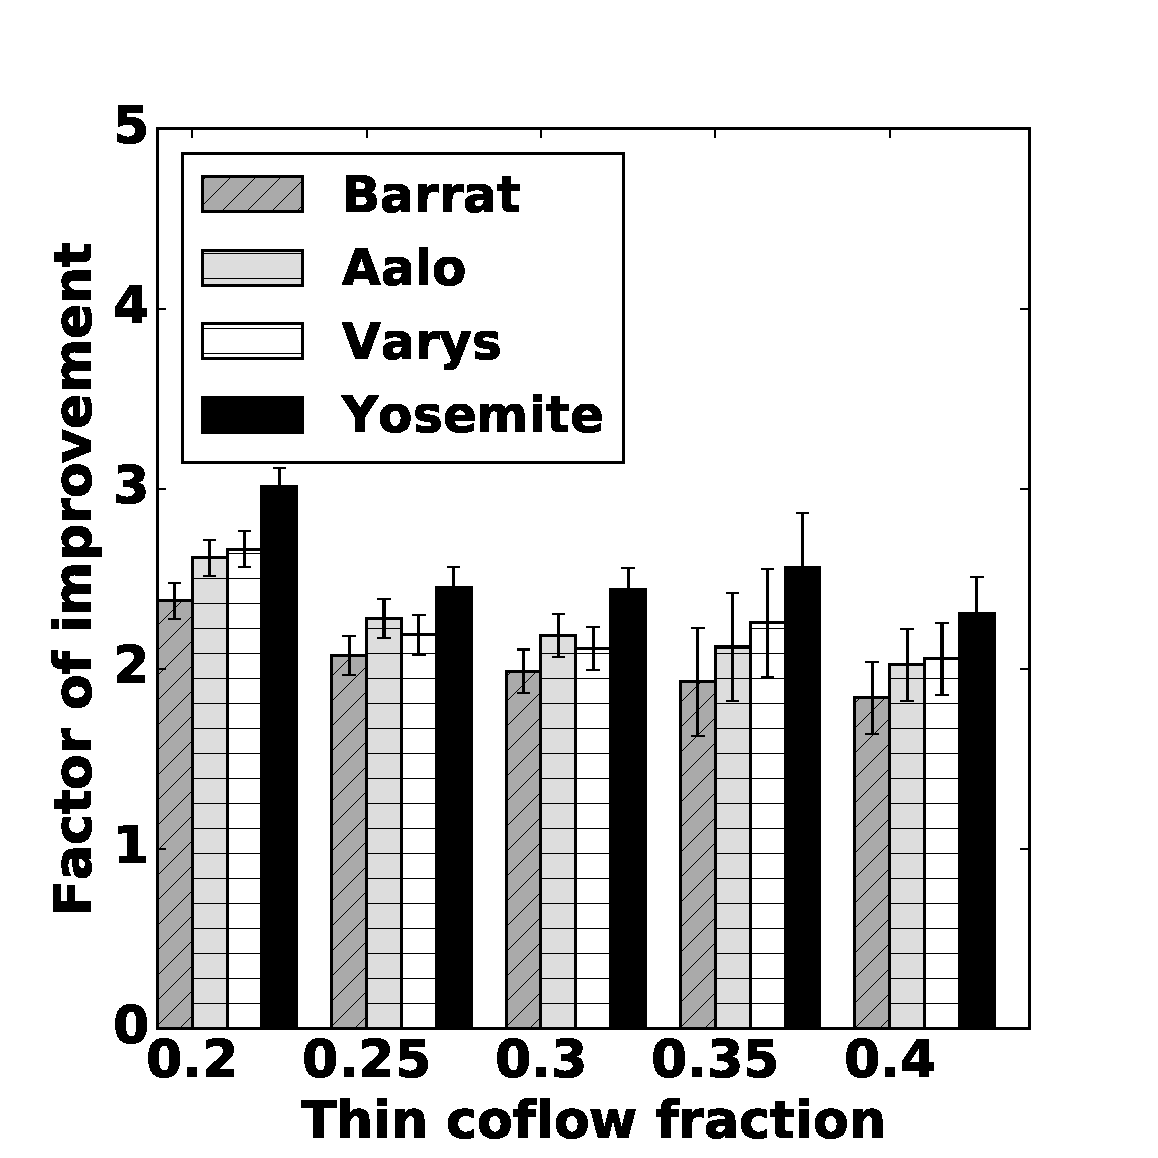
\includegraphics[width=1.65 in]{./figs/different/fracwidth.eps}}
%\hspace{0.1in}
%\subfigure[Impact of coflow weight] {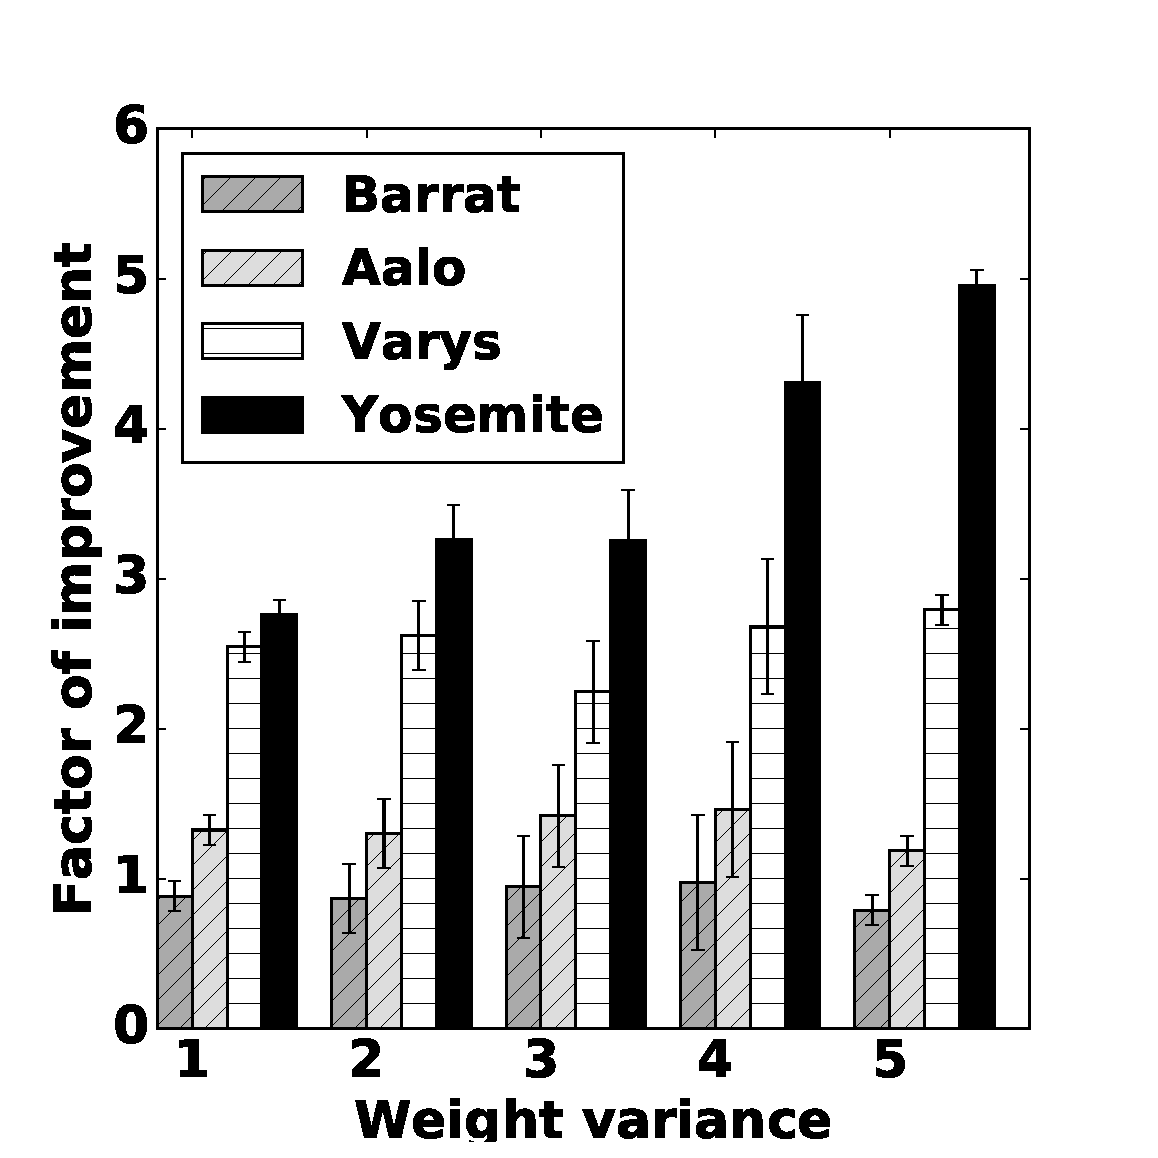
\includegraphics[width=1.65 in]{./figs/different/weight.eps}}
%\vspace{-0.1 in}
%\subfigure[Impact of coflow concurrency] {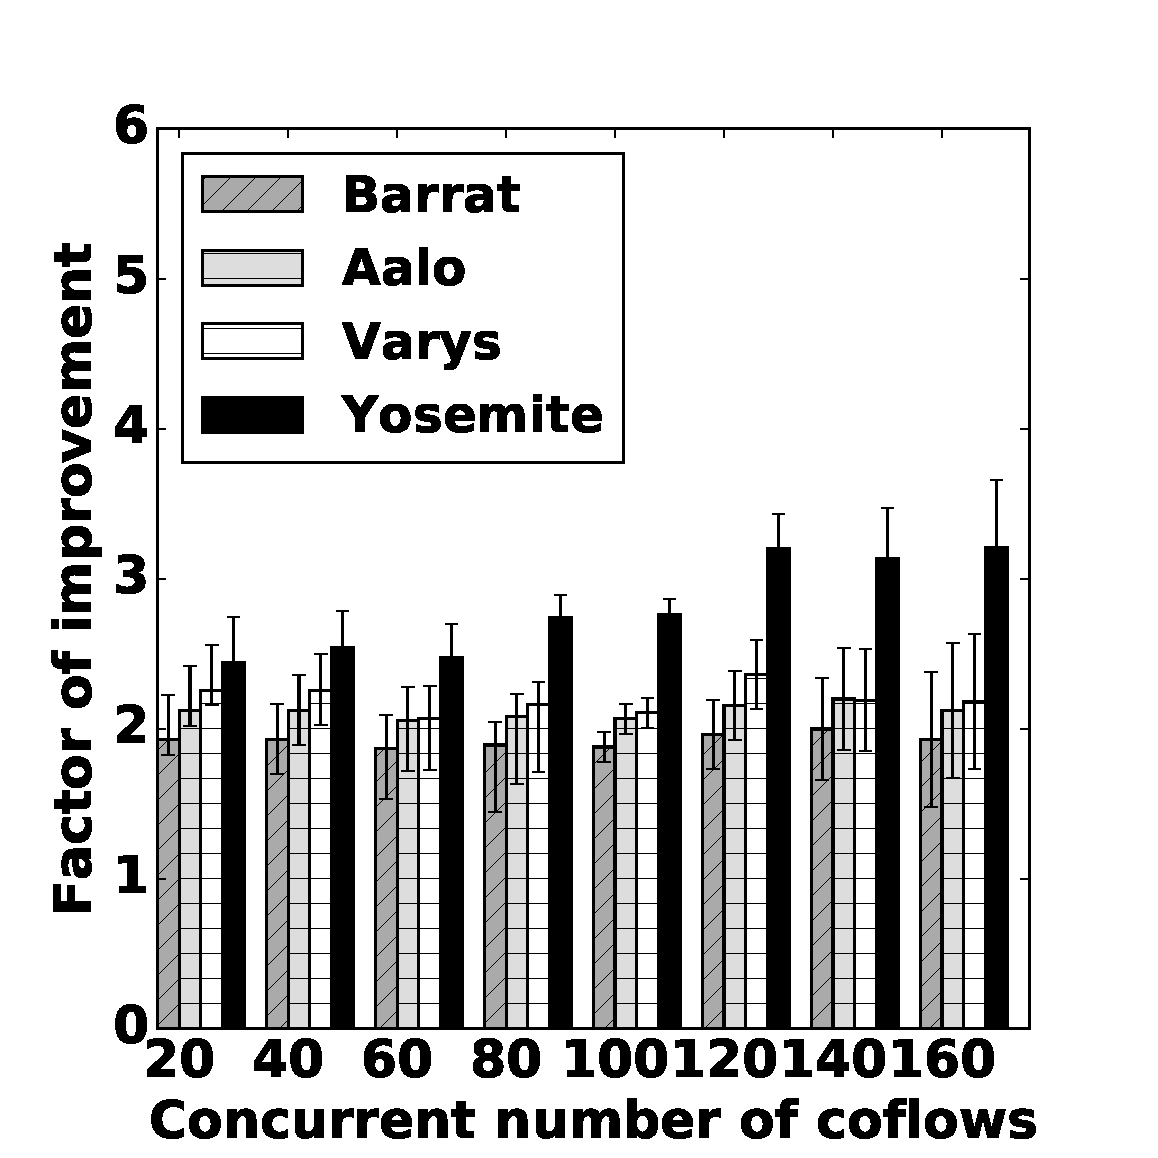
\includegraphics[width=1.65 in]{./figs/different/concurrent.eps}}
%\caption{[Simulation] Yosemite performance comparison with Baraat and Varys, Aalo under different settings.}
%\label{evalution_cases_different_fig}
%\vspace{-0.1 in}
%\end{figure*}
%  \begin{figure}[b]
%\begin{center}
%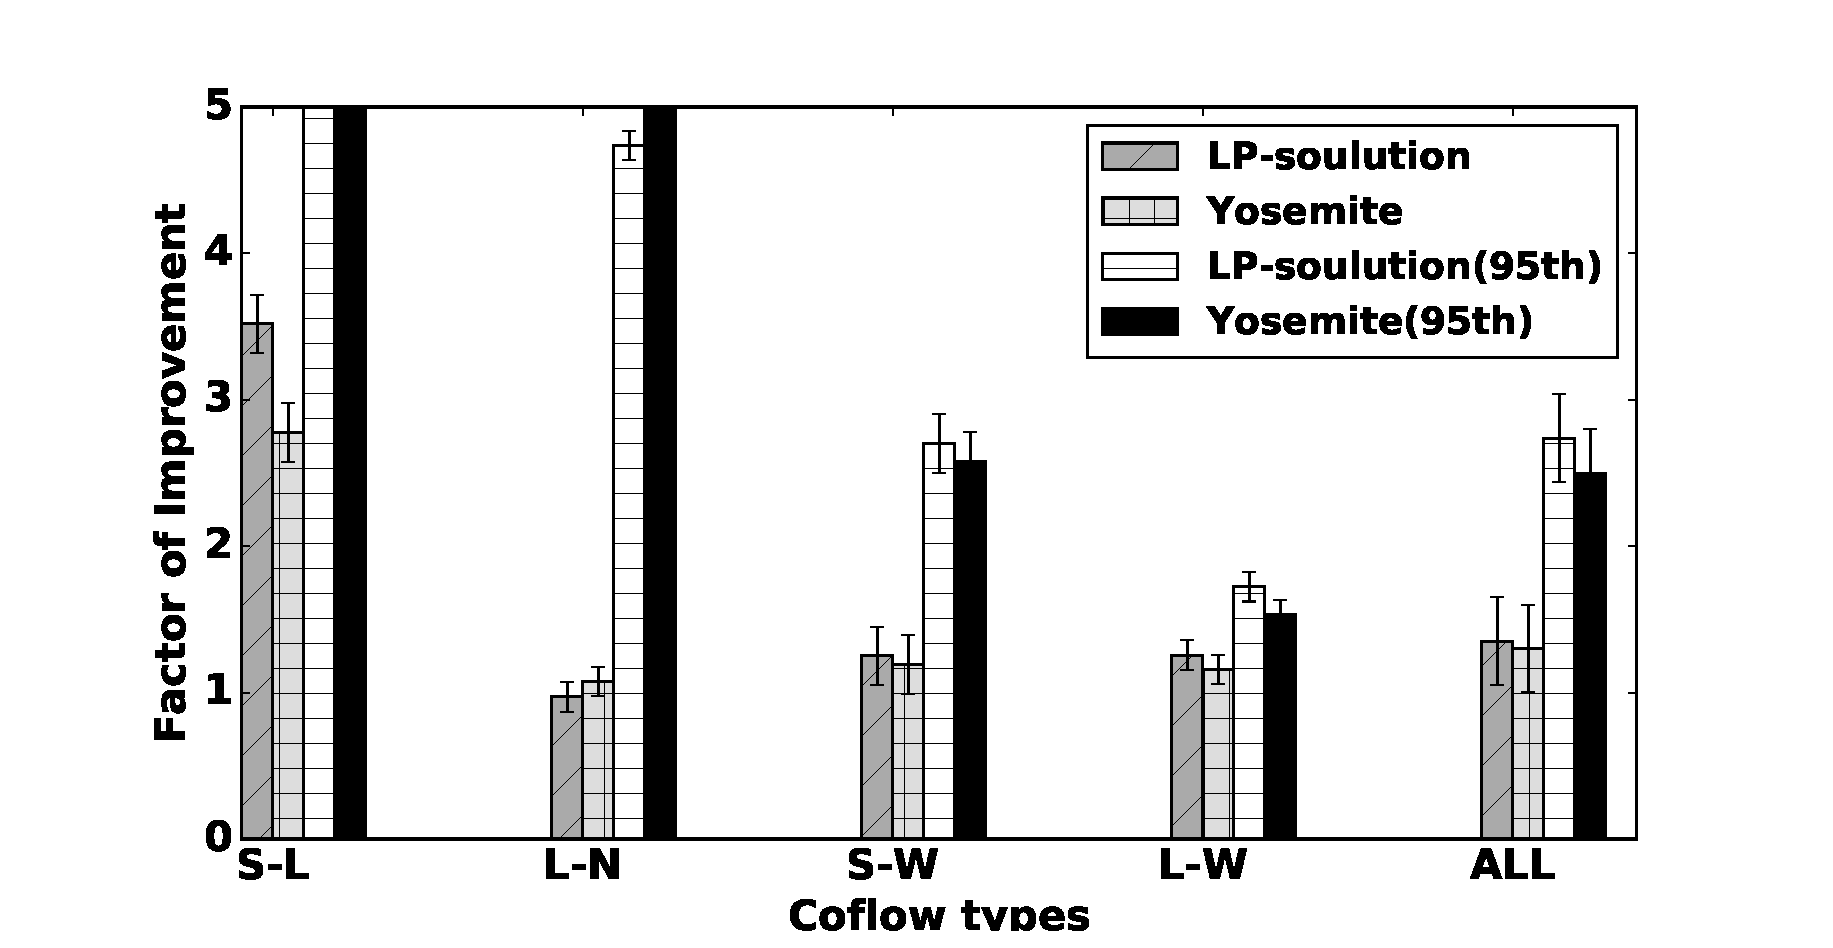
\includegraphics [width=1.0\columnwidth] {./figs/fake/fake1.eps}
%\caption{ [Simulation] Performance comparison between the LP-based solution and Yosemite}
%\label{LP-based-fig}
%\end{center}
%\end{figure}
%%

\textbf{Open source}. To make our experiment repeatable, we publish main codes of Yosemite as well as Yosemite-Sim.
Sources of Yosemite can be downloaded at \cite{Yosemite}.
Main codes of the Yosemite-Sim can be downloaded at \cite{YosemiteSim}.


\subsection{Trace-driven simulation} 
In this section, we use trace of facebook \cite{chowdhury2014efficient} to test the performance of Yosemite.
As the original trace doesn't include weight information, we set random weight within 1, 2, 3, 4, 5 to present the emergence of coflows.
Repeat the process 100 times and Fig. \ref{evaluation_facebook_fig} shows the performance of Yosemite, Barrat, Varys,  Aalo and TCP. 
Note TCP  is selected as the baseline in this group  and repeat the experiment 100 times,
where error bar indicates maximum, minimum and average value. 
To eliminate the influence of extreme value, we remove the top and last $2.5\%$ result of each methods and recompute the factor of improvement, 
so the 95th cases are also shown in the picture.
 
 Fig. \ref{evaluation_facebook_fig}(a) implies that Yosemite greatly reduces the average WCCT across all coflow types. 
 The factors of improvement for Yosemite are 3.5 (Narrow\&Short), 1.6 (Narrow\&Long), 1.7 (Wide\&Short), 1.4  (Wide\&Long) and 1.5 (ALL), 
 while Varys are 2.4 (Narrow\&Short), 0.9 (Narrow\&Long), 1.2 (Wide\&Short), 1.3 (Wide\&Long) and 1.2 (ALL). 
For the 95th case, the improvement factors are (Narrow\&Short),20 (Narrow\&Long), 2.5 (Wide\&Short), 1.5  (Wide\&Long), and 2.5 (ALL), however Varys is 22 (Narrow\&Short),14 (Narrow\&Long), 2.1 (Wide\&Short), 1.2  (Wide\&Long) and 2.1 (ALL) and other 
 method such as Aalo and Barrat performs even worse than Varys.  
Fig. \ref{evaluation_facebook_fig}(b) indicates the distribution of WCCT. 
We can see that more than 80\% WCCT with Yosemite is within 200s, while that for Varys, Aalo, Barrat are 70\%, 65\%, 60\%.
Yosemite performs about 15\%, 25\%, 30\% better than Varys, Aalo and Barrat.

Fig. \ref{evaluation_facebook_fig}(c) shows the average CCT for coflows with different level of emergence.
We can see the factors of improvement for Yosemite are 2.5(Significant), 2.3(Important), 1.2(Normal), 1.4(Unimportant), 1.5(Lax).
While that for Varys are  2.2(Significant), 1.5(Important), 1.4(Normal), 1.6(Unimportant), 1.9(Lax).
For the 95th case, the improvement factors for Yosemite are 3.2(Significant), 3.1(Important), 2.9(Normal), 1.6(Unimportant), 1.9(Lax) and
for Varys are 2.2(Significant), 2.1(Important), 2.0(Normal), 1.9(Unimportant), 2.3(Lax).
We can see Yosemite performs about 20\% better than Varys for the coflows with Significant and Important level,
but for the less important ones, Varys perform about 20\% better than Yosemite.
Fig. \ref{evaluation_facebook_fig}(d) shows the CCT distribution for different methods. 
We can see more than 80\% CCT under Varys is within 20s, while that for Yosemite, Aalo, Barrat are  75\%,65\%,60\%.
Varys performs about 10\% better than Yosemite on minimizing average CCT for all coflows.

We can see that Varys performs better than Aalo, Barrat on minimizing average CCT and average WCCT. 
In the following experiment, we mainly use Varys as the reference method to show the performance of Yosemite.



\subsection{Motivation Resolved}
In this section, we solve the problem that is proposed at Section \ref{background}. 
Applications have 5 level of emergence in our data center and we use 5, 4, 3 ,2, 1 to present the Significant, Important, Normal, Unimportant and Lax level of emergence, then Fig. \ref{evaluation_motivation_fig} shows the result.

Fig. \ref{evaluation_motivation_fig}(a) shows average WCCT for all coflows.
We can see the Normalized WCCT of Varys are 8 (Narrow\&Short), 20(Narrow\&Long), 15 (Wide\&Short), 40  (Wide\&Long) and 30(ALL),
while that for Yosemite are  5 (Narrow\&Short), 15(Narrow\&Long), 10 (Wide\&Short), 30  (Wide\&Long) and 20(ALL).
Yosemite performs about 20\% better than Varys on minimizing average WCCT.
From Fig. \ref{evaluation_motivation_fig}(b) we can see that for vRouter and event which own significant level emergence,
Varys performs almost to TCP, while Yosemite performs about 20\% better than TCP.
For Hadoop and Druid (Important), Yosemite performs about 30\% better than Varys.
While other unimportant applications Varys perform about 10\%$\sim$20\% better than Yosemite.
%As Varys only considers coflow width, coflow length and network condition but ignore the importance of coflows,
%while Yosemite considers both network condition and coflow importance, so that important coflow has higher priority under the same network load.
%For the unimportant, Varys performs better than Yosemite on minimizing average coflow completion time.
Fig.\ref{evaluation_motivation_fig}(c) shows Hadoop average WCCT and Fig.\ref{evaluation_motivation_fig}(d) shows Hadoop CCT.
For index sort and db analysis which are important in our data center, Varys performs even worse than TCP. 
However, using Yosemite, it performs about 30\%$\sim$ 40\% better. 
But for the unimportant and lax coflows, Varys performs better.
For average WCCT,  Yosemite performs about 20\% better than Varys.
%\subsection{Cloud platform evaluation} 
%We deploy Yosemite at our private openstack platform which can start at most 80 virtual machines (2 Cores, 4GB Mem) simultaneously.
%Operation system of each virtual machine is Ubuntu16.04. 
% With the help of Traffic Control module\cite{TC}, we constrain the maximum bandwidth of each VM's NIC to 1GB/s.
% 
% Firstly, we run file distribute application to test the performance of Yosemite.
%Each virtual node constantly construct files whose size ranging from 1KB to 200MB. 
%Weight of each job is randomly generated ranging from 1 to 10.
%Destinations are K nodes which are randomly chosen from the total nodes set.
%Job can be regarded as finished until all the K nodes receive the file. 
%TCP-fair is chosen as the baseline and Fig. \ref{distribute-fig} shows performance comparison between Yosemite and Varys. 
%We repeat the process 10 times and the error bar indicates the max, min and average factor of improvement.
%To decrease the influence of extreme values, we remove the top and last 2.5\% of each methods and recompute the factor of improvement, then we get
%the 95th factor of improvement.
%From  Fig. \ref{distribute-fig}, we can see in total, improvement factor of Yosemite is $3.1$ , while Varys is $2.1$.
%Yosemite improves 30\% better than Varys. 
%The 95th result shows Yosemite performs 31\% better than Varys, which is similar to Varys.
%
%Work conserving aims to allocate the spare network resources to flows, as a result, network resources will be used more efficiently.
%Efficient network utilization will accelerate the transfer process.
%In Yosemite, scheduler allocates the spare bandwidth to flows equally to guarantee the utilization of network resources.
%From Fig. \ref{conserving-fig} , we can see that with work conserving, factor of improvement of Yosemite is 2.1 in total, while that drops to 1.8 without work conserving. 
%
%In reality, scheduler should be fast enough to compute out the scheduler order of coflows.
% Fig. \ref{overheads_fig}(a) shows the computation rate of Yosemite scheduler.
%We can see for peak load, when active coflows is 140,  computation time of the scheduler is $\sim$23ms and
%average computation time is less than 17ms. 
%In our system, more than 90\% file transfers' time are more than 10s.
%We think the average computation time is fast enough to get the schedule result.
%Messages transferring between comm server is the main overheads of Yosemite system.
%Error messages occurs when component crashes and server resources are insufficient.
%As 80 VMs in our platform will reach full load, we start $1\sim 3$ dockers at each VM to get a slightly larger scale experiment.
%Fig. \ref{overheads_fig}(b) shows the error messages frequency. 
%We can see that when the concurrent worker number is over 200, peak error messages is over 4k/s.
%
%
%Write down the trace of distribute file application and let the simulator run the trace under the same parameter.
%Fig. \ref{sim-real} shows the performance gap between Yosemite and trace-driven simulator.
%We can see performance gap between cloud platform and Yosemite is narrow($<15\%$).
%In the following section, we use trace-driven simulator to test performance of Yosemite at larger scale.
%




\begin{figure*}[!t]
\centering
\subfigure[Average WCCT ] {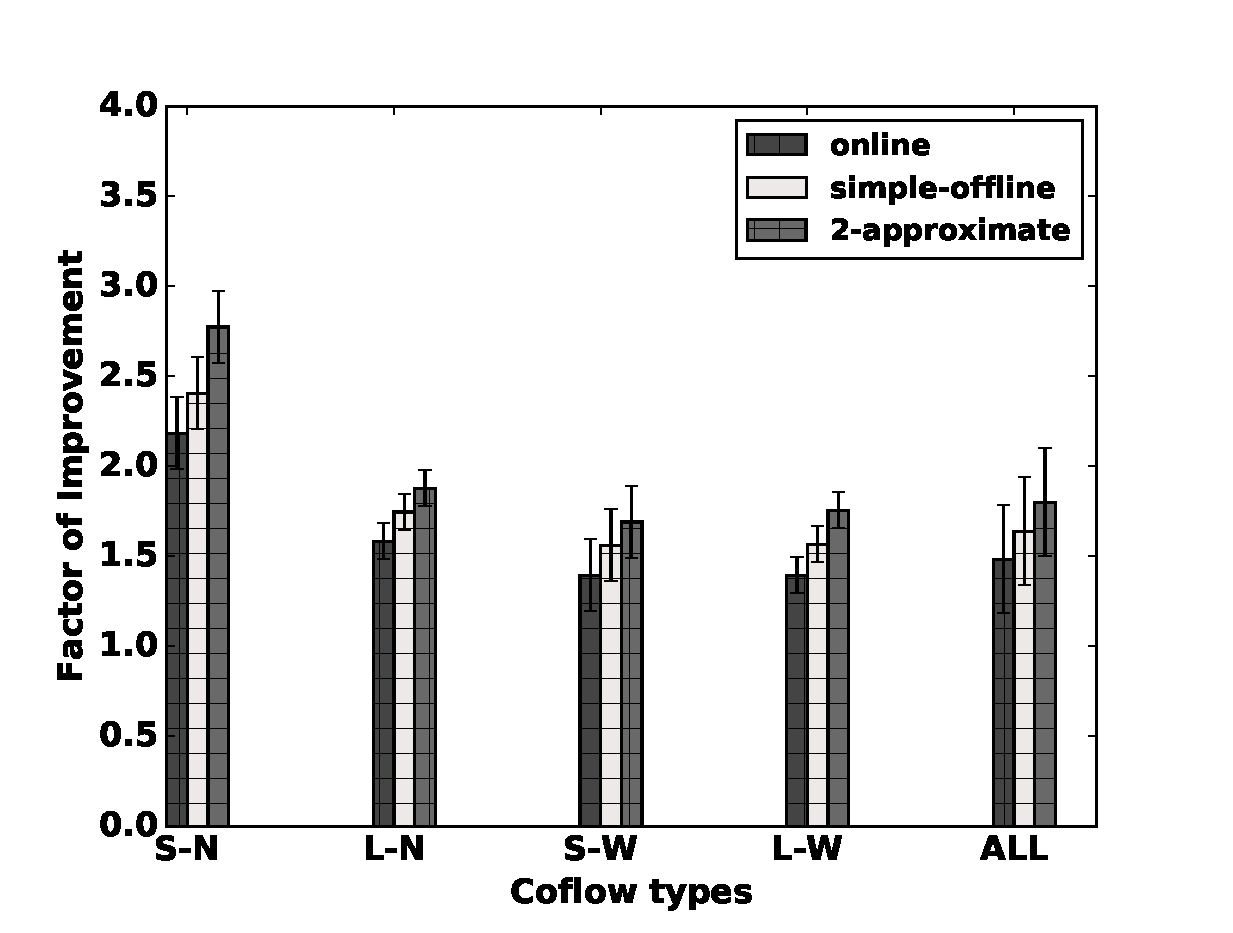
\includegraphics[width=2.1 in]{./figs/performance/nfake5.eps}}
\hspace{0.1in}
\subfigure[Average CCT] {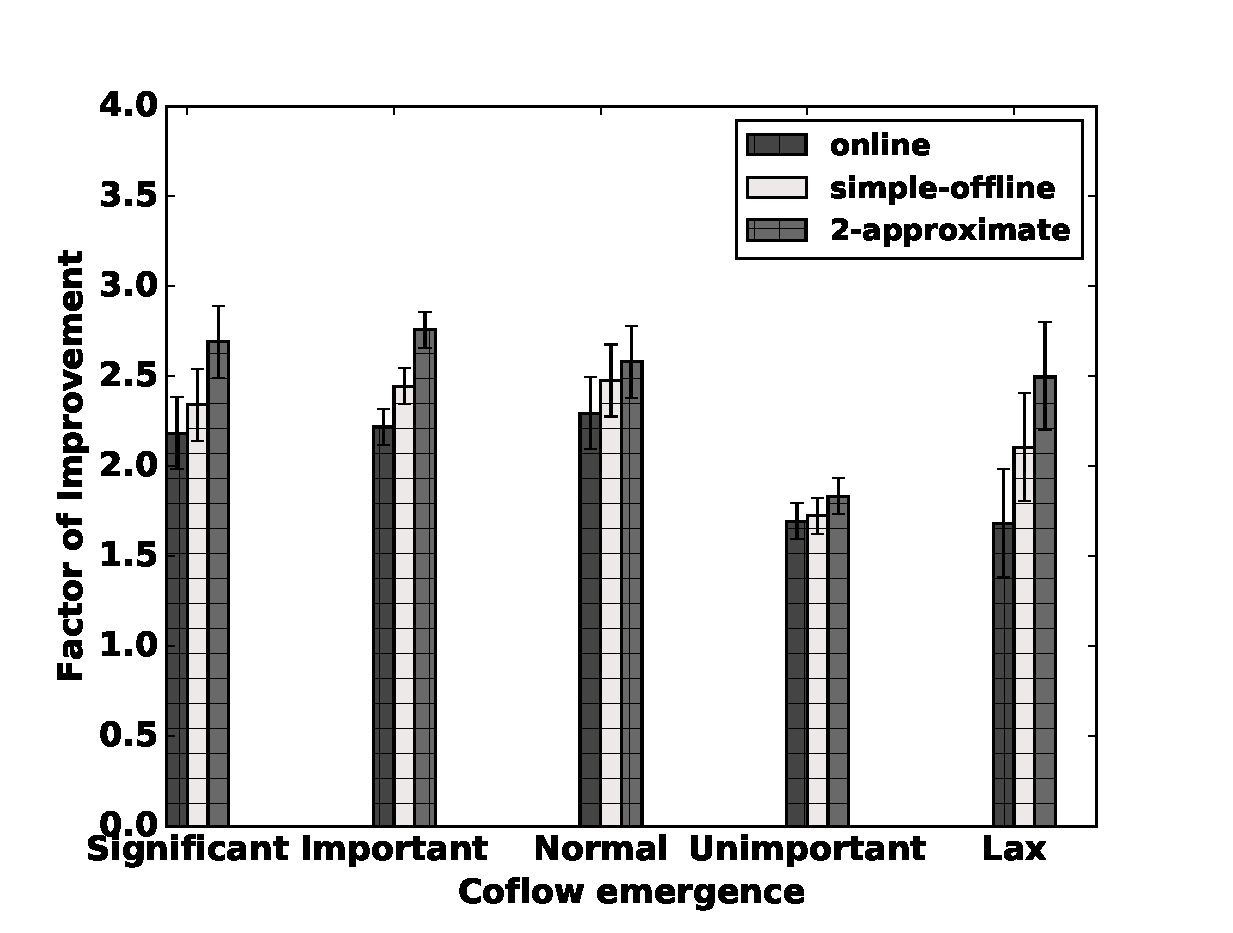
\includegraphics[width=2.1 in]{./figs/performance/nfake4.eps}}
\hspace{0.1in}
\subfigure[CCT distribution] {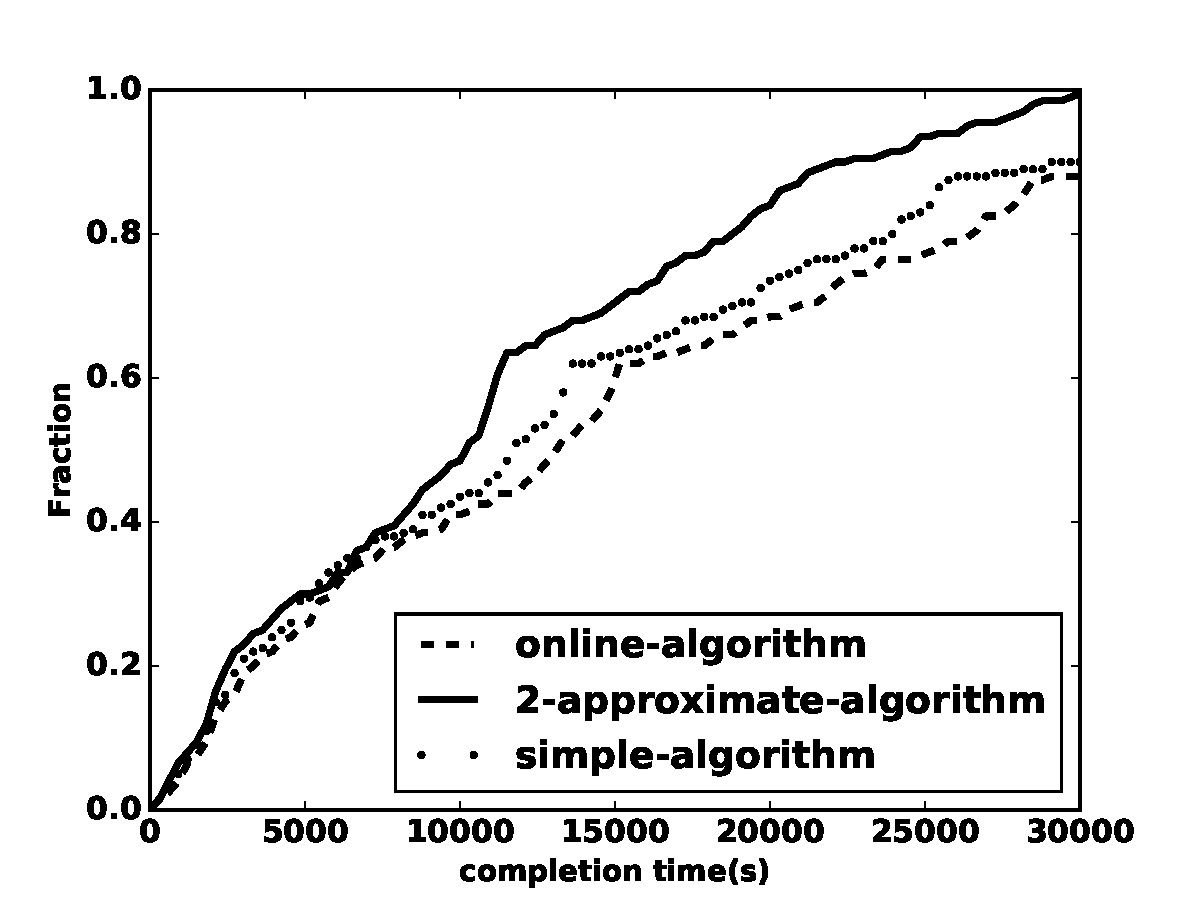
\includegraphics[width=2.1 in]{./figs/performance/online_offline.pdf}}
\vspace{-0.1 in}
\caption{[Simulation] Comparison between the online and offline algorithms, TCP is selected as the baseline}
\label{evaluation_diff_fig}
\vspace{-0.1 in}
\end{figure*}
\begin{figure*}[!t]
\centering
\subfigure[Average CCT] {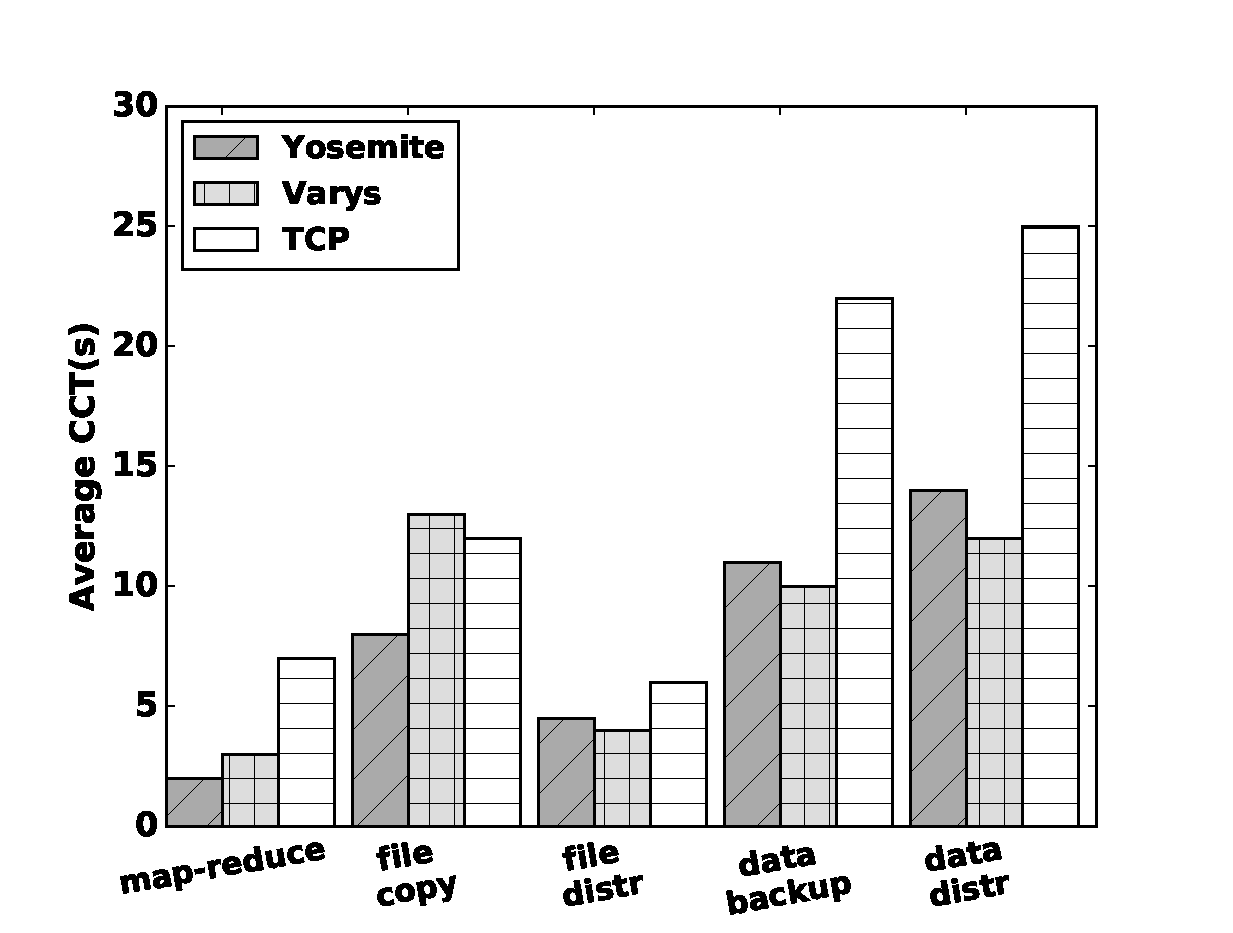
\includegraphics[width=1.65 in]{./figs/evaluation/ex5/real1.eps}}
\hspace{0.1in}
\subfigure[Average CCT (95th)] {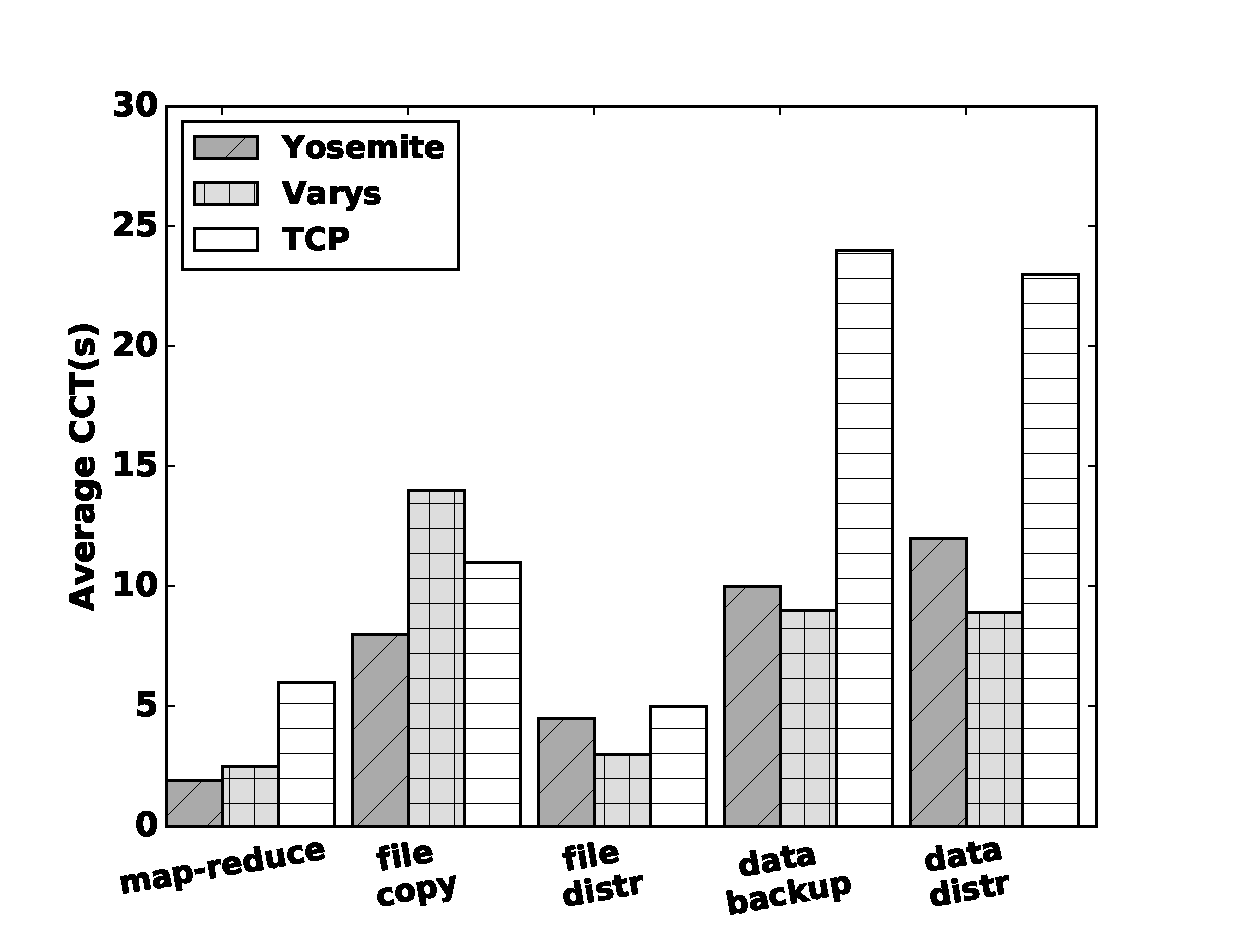
\includegraphics[width=1.65 in]{./figs/evaluation/ex5/real2.eps}}
\vspace{-0.1 in}
\subfigure[file-dist CCT ] {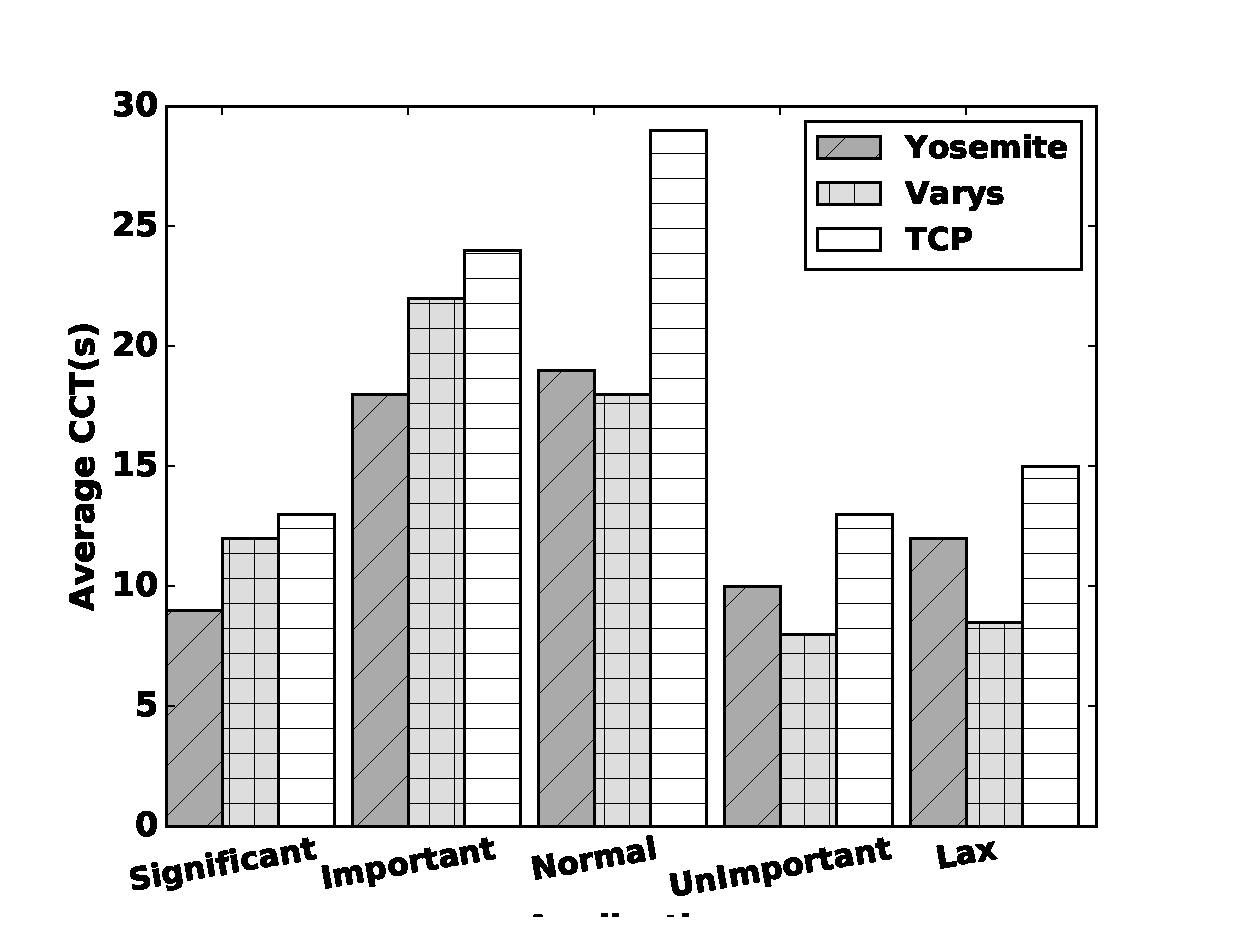
\includegraphics[width=1.65 in]{./figs/evaluation/ex5/real3.eps}}
\hspace{0.1in}
\subfigure[file-dist CCT (95th)] {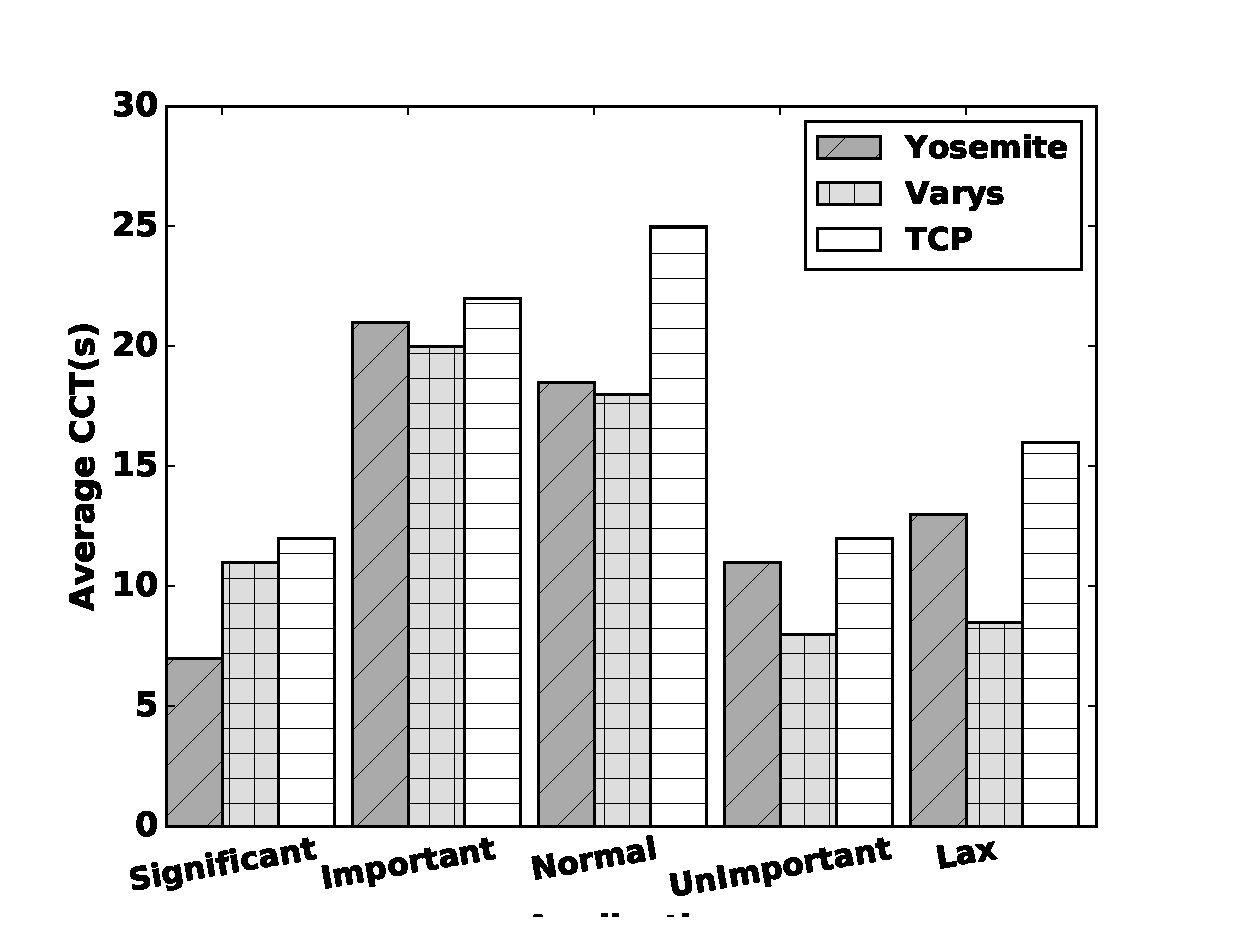
\includegraphics[width=1.65 in]{./figs/evaluation/ex5/real4.eps}}
\hspace{0.1in}
\caption{[Testbed] Performance under different applications in openstack}
\label{evaluation_cloud_fig}
\vspace{-0.1 in}
\end{figure*}



 \begin{figure*}[!t]
\centering
\subfigure[Average WCCT comparison] {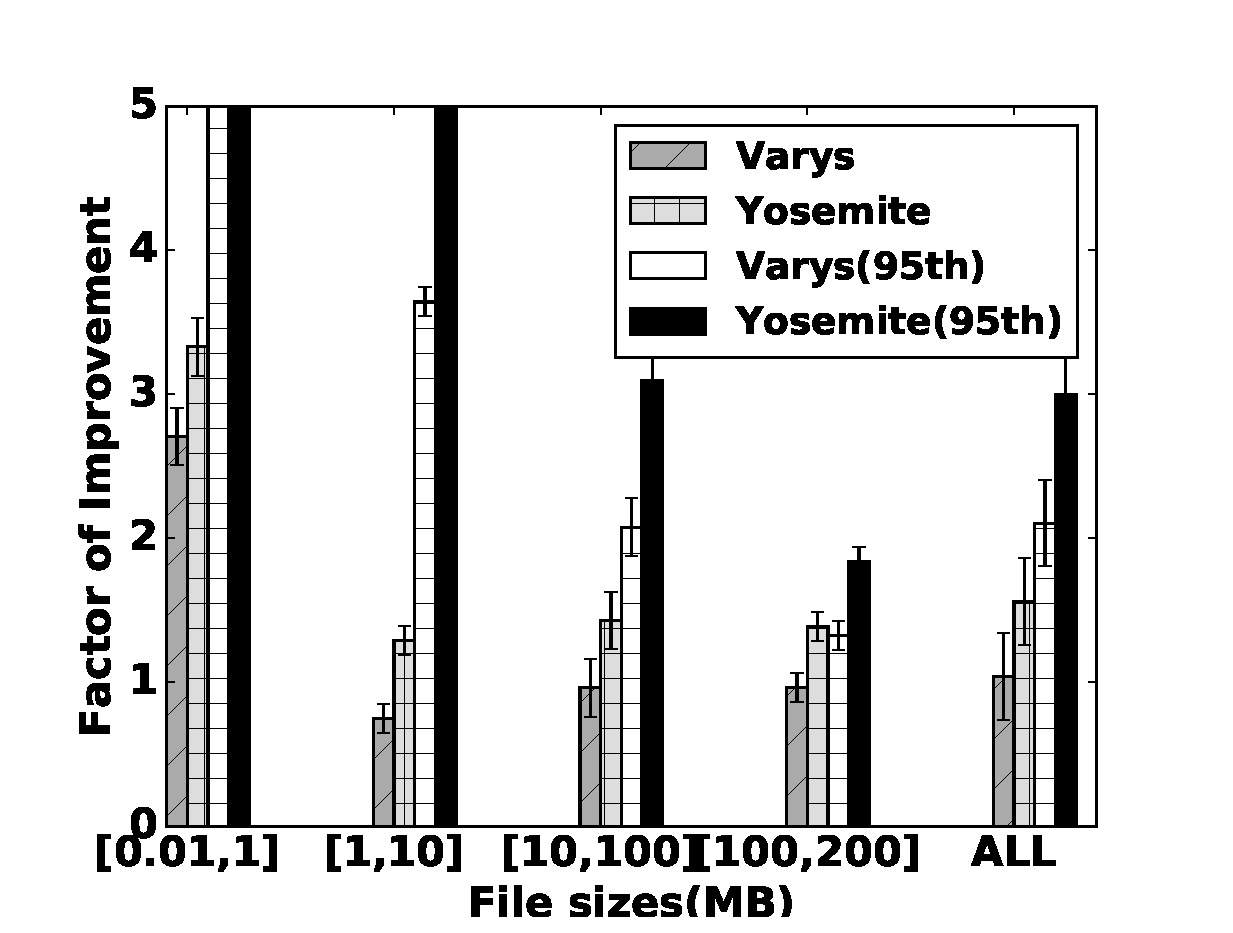
\includegraphics[width=2.1 in]{./figs/fake/fake2.eps}}
\hspace{0.1in}
\subfigure[Computation time of scheduler] {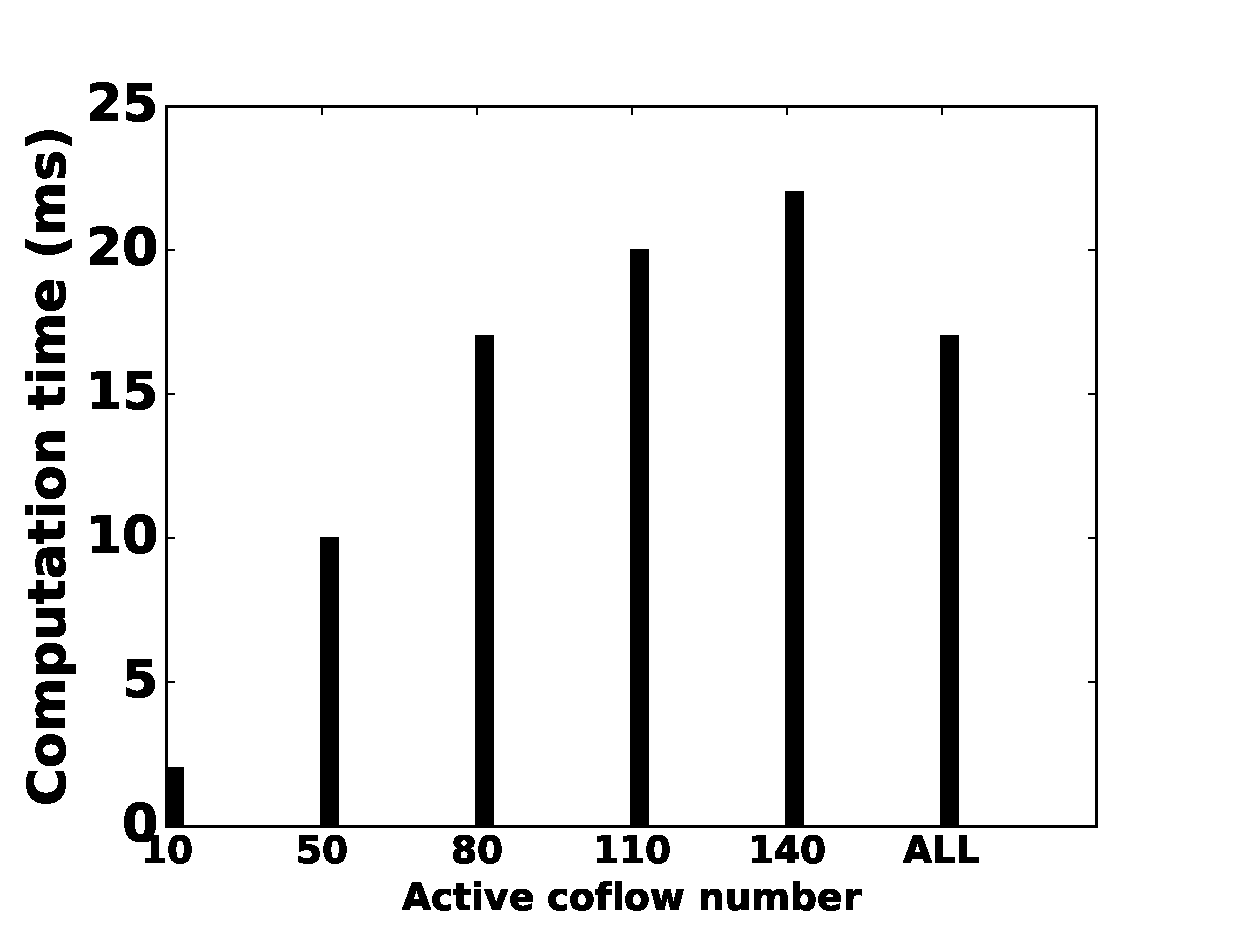
\includegraphics[width=2.1 in]{./figs/fake/fake5.eps}}
\hspace{0.1in}
\subfigure[Testbed and Simulator comparison] {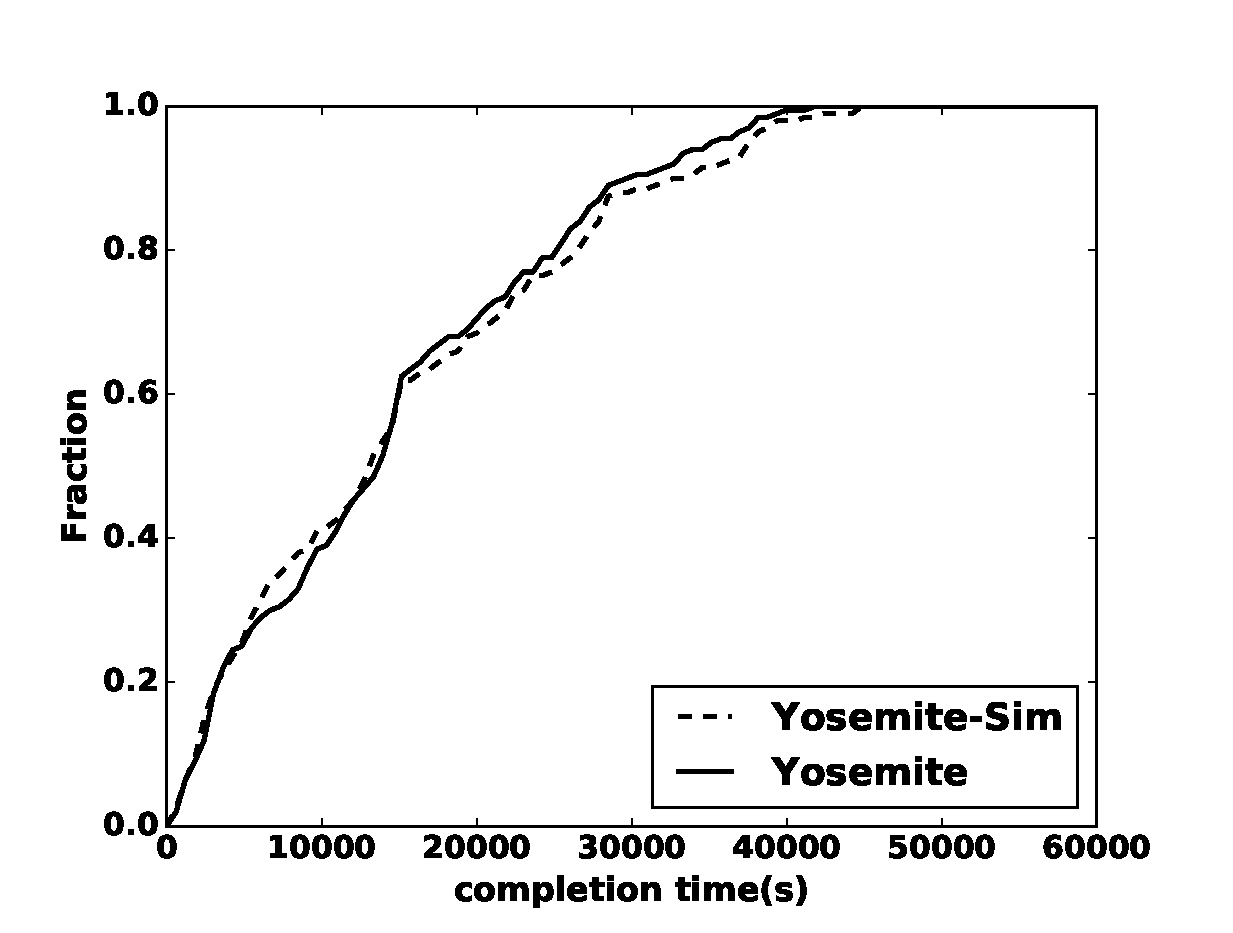
\includegraphics[width=2.1 in] {./figs/fake/fake3.eps}}
\caption{[Testbed] Some details of Yosemite}
\label{overheads_fig}
\vspace{-0.1 in}
\end{figure*}


%\begin{eqnarray} \label{improvement}
%Factor \;of\; improvement=\frac{baseline\; avg \;WCCT}{current\;avg \;WCCT}
%\end{eqnarray}
%Note, in this paper, we use TCP-fair sharing as the default baseline method.
%\begin{figure}[b]
%\begin{center}
%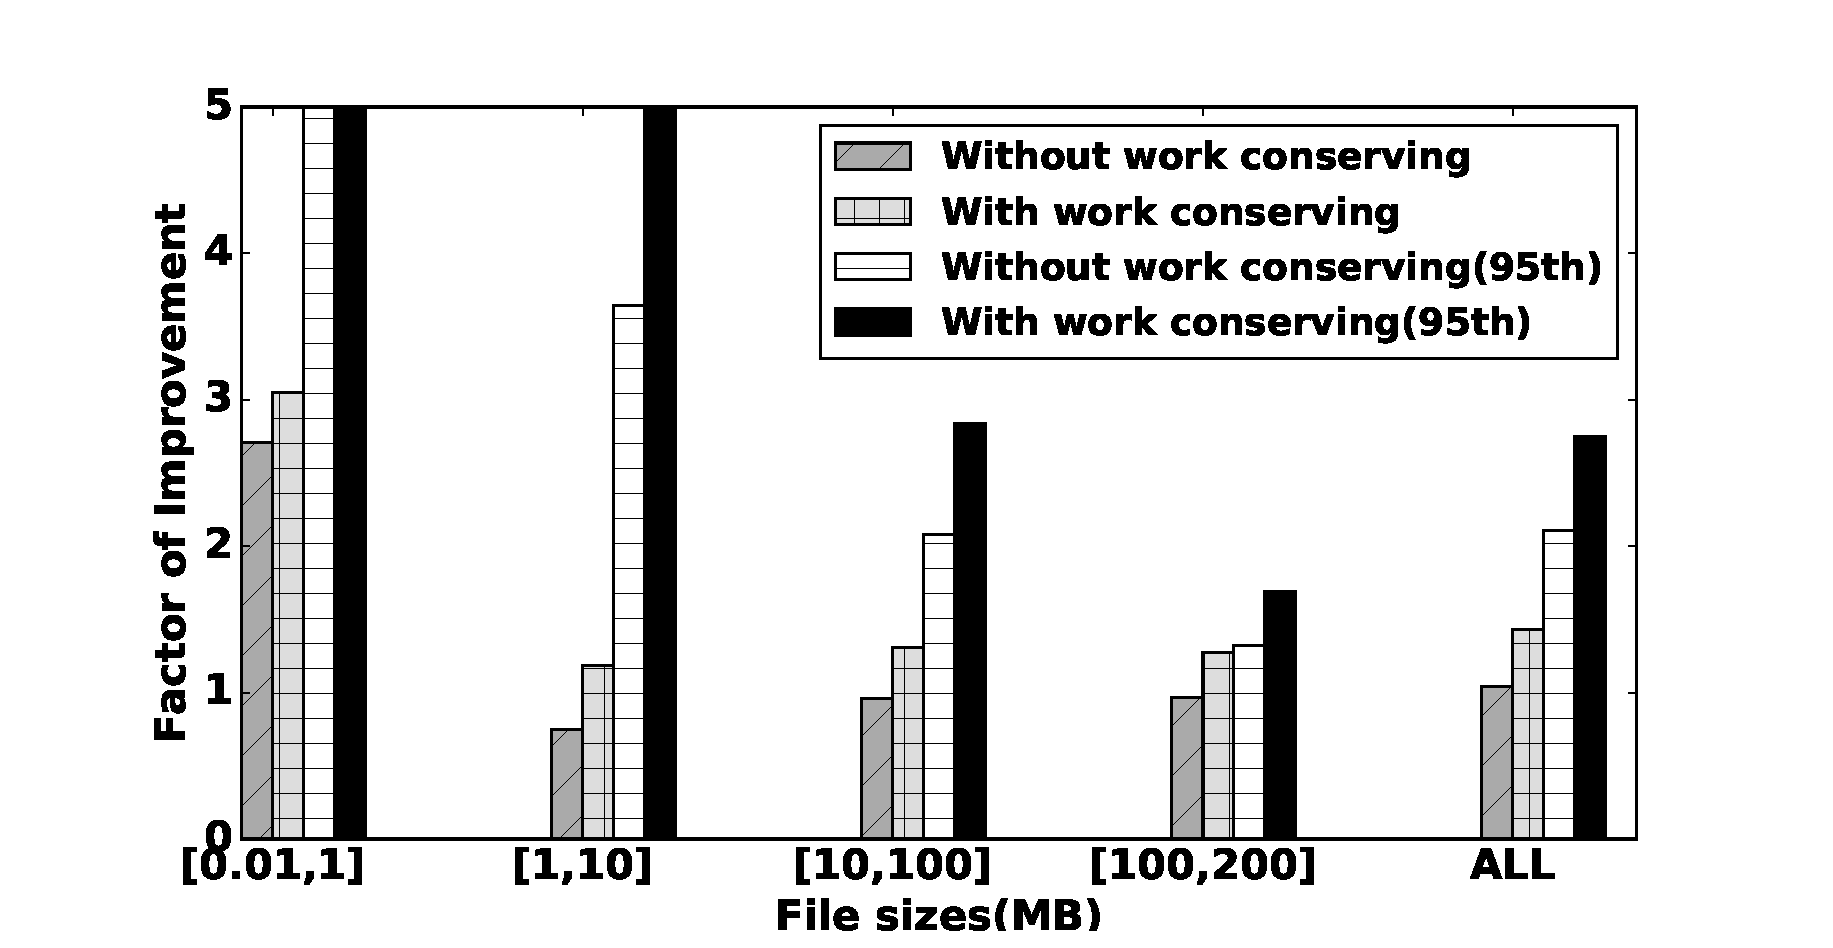
\includegraphics [width=1.0\columnwidth] {./figs/fake/fake4.eps}
%\caption{[Cloud] With and without work conserving}
%\label{conserving-fig}
%\end{center}
%\end{figure}

\subsection{How to set weight in practice} 
Weight plays an important role in Yosemite scheduling system.
Adjacent weight difference is 1 in our prior experiments.
In this group, we use facebook trace and set weight within 1,1+wd,1+2*wd,1+3*wd,1+4*wd.
Change wd from 1 to 10 and Fig.\ref{evaluation_weight_fig}(a) shows the average WCCT, important coflows' ($weight> 1+2*wd$) average CCT.
We can see that with the increasing of weight difference, improvement of average WCCT increases, but average CCT for important coflows almost remains the same.
We can explain that Yosemite uses weight and accumulated data to decide the rank factor.
With a larger weight difference, weight plays an more important role and the influence of accumulated data becomes smaller.  
Fig.\ref{evaluation_weight_fig}(c) shows the result of larger wd difference, where wd ranges from 2 to 64.
We can see when wd $>$ 8, improvement of cct for important coflows becomes small and this is similar to Fig.\ref{evaluation_weight_fig}(a).

In practice, we can set weight by the demands of network administrator.
When we regard the emergence of coflows as the key schedule factor, we can use large wd.
When we think both the emergence level of coflows and network condition are the key factors, we can use small wd.

\subsection{Distance between online and offline} 
Simple-offline algorithm ignores load difference of each port and online algorithm further assumes that larger coflows that last long time and should have low priority.
To see the performance loss,  we consider the schedule of 100 coflows served by a small-scale cluster consisting of 60 hosts. 
Let all the coflow start at t = 0 and set weight random within 1 , 2 , 3 , 4 ,5.
Then repeat the process 100 times and Fig. \ref{evaluation_diff_fig} shows the result.
From Fig. \ref{evaluation_diff_fig}(a), we can see that factor of Improvement for WCCT of the online method is 1.6. 
While that for simple-offline method is 1.7 and the 2-approximate method is 1.8.
Comparing with the 2-approximate algorithm, the online algorithm has about 10\% performance loss on minimizing average WCCT.
Fig. \ref{evaluation_diff_fig}(b) shows the performance for different emergence level of coflows.
We can see that comparing with 2-approximate algorithm, the online method has about 30\% performance loss.
Fig. \ref{evaluation_diff_fig}(c) shows the distribution for CCT. 
We can see more than 80\% CCT for 2-approximate method is within 20000s, while that for simple-offline and online methods are 70\% and 60\%.
%
%From Fig. \ref{online-offline-fig}, we can see the online algorithm performs close to the 2-approximate algorithms in total and only prolongs the transfer of large coflows. 
%As coflows are generated randomly, we repeat the numerical simulation 200 times. 
%Table \ref{tab:loss} shows the proportions of $\frac{avg \;wcct\  of \ online}{avg\; wcct \ of \  2-appr}-1$, where $avg\;wcct $ means average weighted coflow completion time.
%We can see that 64\% cases have less than 0.025 of performance loss.
%More than 91\% cases have less than 0.1 performance gap and no cases have more than 0.15 performance loss.  
%
%      \begin{table}[!htb]
%          \centering
%          \footnotesize
%          \caption{Performance loss result} \label{tab:loss}
%          \begin{tabulary}{\textwidth}{cccccr}
%              \toprule
%              $\leq 0\%$  & \multicolumn{1}{c}{$\leq 0.025$} & $\leq 0.05$& $\leq 0.1$ &$\leq 0.15$\\
%              \midrule
%              \multicolumn{1}{r}{0} & 64\%    &72\%    &91\%  &100\%  \\
%             \bottomrule
%          \end{tabulary}
%      \end{table}
      
      
%\begin{table}[!htb]
%          \centering
%          \footnotesize
%          \caption{Comparison between the three algorithms} \label{tab:comparison}
%          \begin{tabulary}{\textwidth}{ccccr}
%              \toprule
%              \#Scheme  & \multicolumn{1}{c}{Mode} & Procedure & Performance &information\\
%              \midrule
%              \multicolumn{1}{r}{2-approximate} & offline    & Complex     & High &clairvoyant\\
%              \multicolumn{1}{r}{simple-offline} & offline    & simple     & High& clairvoyant \\
%              \multicolumn{1}{r}{Yosemite} & online    & simple     & High & non-clairvoyant\\
%              \bottomrule
%          \end{tabulary}
%      \end{table}
%      
%
%As Table. \ref{tab:comparison} shown, we conclude comparing with the offline algorithm, online algorithm has little performance loss. 
%Indeed, it is much more simple and can maintain relative high performance,
%so that in reality, using the online algorithm to schedule coflow is a good choice.


\subsection{Real testbed evaluation} 
We deploy Yosemite at our private openstack platform which can start at most 80 virtual machines (2 Cores, 4GB Mem) simultaneously.
Operation system of each virtual machine is Ubuntu16.04. 
 With the help of Traffic Control module\cite{TC}, we constrain the maximum bandwidth of each VM's NIC to 1GB/s.
 
 Firstly, we deploy 5 applications in our data center: map-reduce, file-copy, file-distribute, data-backup, data-distribute. 
 Emergence of the 5 applications are in turn: Significant, Important, Normal, Unimportant, Lax.
 Fig. \ref{evaluation_cloud_fig}(a) shows the total result and Fig. \ref{evaluation_cloud_fig}(b) shows the 95th percentile.
 We can see for map-reduce and file-copy which have high level of emergence, Yosemite performs about 20\% $
 \sim$ 30\% better than Varys, but for the unimportant applications, Yosemite performs about 20\% worse than Varys.
 Fig. \ref{evaluation_cloud_fig}(c) shows the performance for file-distribution.
 Set five important level to files, we can see that Yosemite performs about 20\% better than Varys. 
 The 95th percentile result, as Fig. \ref{evaluation_cloud_fig}(d) shown, is similar. 
 
Then for the file distribution application, we let each virtual node constantly construct files whose size ranging from 1KB to 200MB. 
Destinations are nodes which are randomly chosen from the total nodes set and Fig. \ref{overheads_fig} shows performance comparison between Yosemite and Varys. 
We repeat the process 10 times and the error bar indicates the max, min and average factor of improvement.
From  Fig. \ref{overheads_fig}(a), we can see factor of improvement for Yosemite is $3.1$ , while Varys is $2.1$.
Yosemite improves 30\% better than Varys. 

In reality, scheduler should be fast enough to compute out the scheduler order of coflows.
 Fig. \ref{overheads_fig}(b) shows the computation rate of Yosemite scheduler.
We can see for peak load, when active coflows is 140,  computation time of the scheduler is $\sim$23ms and
average computation time is less than 17ms. 
In our system, more than 90\% file transfers' time are more than 10s.
We think the average computation time is fast enough to get the schedule result.

 Fig. \ref{overheads_fig}(c) shows the result comparison for the simulator and real testbed.
 In this experiment, we use the same parameters just as the file distribution.
 We can see that the total performance gap between the two methods are about 20\%.
 This result shows the credibility of our simulation. 




% Fig. \ref{evalution_real_fig} shows cct performance of Yosemite, Barrat, Varys,  Aalo, TCP-fair sharing with the same settings, TCP-fair sharing is selected as the baseline. 
%Fig. \ref{evalution_real_fig}(a) shows that the improvement factors of Yosemite on cct  are 2 (Narrow\&Short),1.1 (Narrow\&Long), 0.8  (Wide\&Short), 0.9   (Wide\&Long) and 1.3 (ALL) , while Varys performs about $\sim5\%$ better than Yosemite. 
% Fig. \ref{evalution_real_fig}(a) also shows the maximum value and minimum value of Yosemite under different weight settings. 
% For Barrat, Aalo and Varys, as their cct have no relationships with weight, so that average cct  will not change under different weight settings.  
% Fig. \ref{evalution_real_fig}(b) shows the result of distribution of coflow completion time which is similar to Fig. \ref{evalution_real_weight_fig}(b).
% 
% 
% \subsection{Performance under different settings} 
% In this section, we explore the performance of Yosemite under different settings. 
%From Algorithm \ref{online-algorithm},  we can see performance of Yosemite is mainly influenced by coflow length, coflow width, coflow weight and coflow concurrency. 
% In this part, we explore Yosemite's performance from the four aspects.
% 
% \begin{table}[!htb]
%          \centering
%          \footnotesize
%          \caption{Default parameters in each group of experiment} \label{tab:parameters}
%          \begin{tabulary}{\textwidth}{cccccr}
%              \toprule
%               Number &Length & Width & Weight & Arrival&Capacity\\
%              \midrule
%              \multicolumn{1}{r}{512}&[100KB,10GB]   &60& [1,10]  & [0s,1000s]&10GB/s\\
%              \bottomrule
%          \end{tabulary}
%      \end{table}
%      
% 
%In each group of experiment, we fix the value of other parameters and only change the factor we want to study. 
%Table \ref{tab:parameters} shows the default settings of parameters. 
%We start 512 coflows in each group of experiment and length of each coflow are within 100KB to 10GB. 
%Width of each coflows are at most 60 and weight of each coflows are within 1 to 10. 
%coflow's arrival time ranges 0s to 1000s. 
%Ingress and egress port capacity in our experiment are 10GB/s. 
%We repeat each group of experiments 100 times and draw maximum, minimum as well as average value pictures.
%
% \subsubsection{Impact of coflow length}
% In this group of experiment, we test the influence of coflow length.
% Coflow width, weight, arrival time are set as Table \ref{tab:parameters} shown. 
% In each group of experiment, we only change length of coflow.  
% Coflow length in our experiment are set within [100KB,K]. 
% Varying K from 1GB to 6GB. 
% Fig. \ref{evalution_cases_different_fig}(a) shows the result. 
% From Fig. \ref{evalution_cases_different_fig}(a) we can see that with the increasing of K, improvement of Yosemite becomes larger. 
% For example, when K is 1GB,  improvement of Yosemite is 2 and when K is 6GB, improvement of Yosemite is 3. 
%Indeed, when K becomes larger, length differentiation between coflows becomes larger, scheduling result is better.
% 
% \subsubsection{Impact of coflow width}
%Fig. \ref{evalution_cases_different_fig}(b) shows the influence of coflow width.  
%In this group of experiment, we vary the fraction of thin coflows (width$<$ 30) from 20\% to 40\%.
%Coflow length, width, as well as coflow arrival time are set as Table \ref{tab:parameters} shown. 
%From  Fig. \ref{evalution_cases_different_fig}(b), we can see that with the increasing fraction of thin coflows,  improvement of Yosemite becomes smaller.  
%The reason for this is that, when fraction of thin coflows is small, conflict probability between coflows is large, so it is necessary to decide a suitable scheduling sequence of coflows.
% 
% \subsubsection{Impact of coflow weight}
% Weight indicates the importance of the application in reality. 
% Weight setting has huge influence on the performance of weighted coflow completion time. 
% In this section, we study the influence of weight. 
% Coflow length, width and arrival time are set according to Table \ref{tab:parameters}.
%Weight are generated within $[8-\sigma,8+\sigma]$, varying $\sigma$ from 1 to 5 and
%Fig. \ref{evalution_cases_different_fig}(c) shows the result. 
%From Fig. \ref{evalution_cases_different_fig}(c), we can see that when weight variance $\sigma$ becomes larger, improvement of Yosemite becomes larger. 
%This means Yosemite works better for larger weight variance cases.
% 
% \subsubsection{Impact of coflow concurrency}
%In real word, coflow can start at any time. 
%Arrival time of coflows can impact the traffic load in data center network. In this part, we explore the impact of coflow concurrency. 
%Changing the number of coflows that start at time 0. 
%Fig. \ref{evalution_cases_different_fig}(d) shows the result. 
%We can see that with the concurrent number of coflows increasing, improvement of Yosemite becomes larger.  
%The reason for this is that when workload becomes heavier, the optimization space for preemptive scheduling become larger.
  
%  \subsection{Distance to Optimization}
% 
%It is hard to find the optimal schedule, so that we find an LP-based solution \cite{qiu2015minimizing} whose approximation ratio is
%$\frac{67}{3}$ to compare with. 
%Use facebook trace and generate weight within 1 to 5, then repeat the experiment 20 times and Fig. \ref{LP-based-fig} shows the result. 
%We can see that Yosemite has less than 10\% performance gap.
 
 \section{Conclusion} \label{conclusion}
 In this paper, we use weight to quantify the emergence of applications.  
Coflows belonging to emergent applications own large weight.
We design and implement Yosemite-a coflow scheduling system that aims to minimize average weighted coflow completion time.
We test the performance of it by trace-driven simulation and test-bed deployment.
Experiments show Yosemite can reduce average weighted coflow completion time significantly.  
Methods of Yosemite is clairvoyant, which means that flow size do not need to know beforehand.
This makes the method widely used in practice.
In our experiment, we use 5 level of importance, however, in practice, thin granularity of emergence may be needed.
Also, we use 1, 2, 3, 4, 5 as the default weight, indeed, more accuracy weight setting can be set to improve the performance of Yosemite.
In the future, we will discuss how to set weight from theory.



\bibliographystyle{abbrv}
\bibliography{paper}



\end{document}



